% !TeX program = pdflatex
% =====================================================================
%  PIPELINE MODULAR PARA DETECÇÃO DE ÁUDIO SINTÉTICO
%  Versão consolidada e refatorada — Thierry Gonçalves Braga
%  - Arquiteturas nomeadas conforme a literatura
%  - 11 modelos consolidados: WavLM Original, HuBERT Original, RawNet2, AASIST,
%    RawGAT-ST, Conformer, CCT, AST, Res2Net, SVM e Random Forest
%    (o sufixo "Original" distingue os SSL reais do porte Keras do escopo
%     estendido; AST/CCT/Res2Net mapeiam para SpectrogramTransformer/
%     Hybrid CNN-Transformer/MultiscaleCNN no repositorio -- ver tab:aliases)
%  - Tabelas/figuras de benchmark geradas automaticamente (tabelas_benchmark.tex)
% =====================================================================
\documentclass[12pt,a4paper]{article}

% =====================================================================
%  PACOTES ESSENCIAIS
% =====================================================================
\usepackage[brazilian]{babel}
\usepackage[utf8]{inputenc}
\usepackage[T1]{fontenc}
\usepackage{lmodern}
\usepackage{graphicx}
\usepackage{cite}
\usepackage{amsmath}
\usepackage{amssymb}
\usepackage{indentfirst}
\usepackage{geometry}
\usepackage{booktabs}
\usepackage{multirow}
\usepackage{array}
\usepackage{subcaption}
\usepackage{float}
\usepackage{xcolor}
\usepackage{tikz}
\usepackage{tcolorbox}
\usepackage{fancyhdr}
\usepackage{titlesec}
\usepackage{enumitem}
\usepackage{microtype}
\microtypesetup{expansion=false}
\usepackage{url}
\usepackage{setspace}
\usepackage{caption}
% siunitx real: disponível em qualquer instalação TeX Live completa.
% \num/\SI seguem a convenção pt-BR (decimal
% por vírgula, milhar por ponto a partir de 5 dígitos); unidades
% kilo/hertz/second/milli/percent já são nativas do pacote.
\usepackage{siunitx}
\sisetup{
  output-decimal-marker = {,},
  input-decimal-markers = {,},
  group-separator       = {.},
  group-minimum-digits  = 5
}
\DeclareSIUnit{\decibel}{dB}
\DeclareSIUnit{\bit}{bit}
\DeclareSIUnit{\dBFS}{dBFS}
\DeclareSIUnit{\megabyte}{MB}
\usepackage{hyperref} % deve ser o último

% =====================================================================
%  ESPAÇAMENTO ABNT (NBR 14724)
% =====================================================================
\onehalfspacing
\frenchspacing

% =====================================================================
%  TIKZ
% =====================================================================
\usetikzlibrary{shapes.geometric, arrows, positioning, fit}

% =====================================================================
%  CORES
% =====================================================================
\definecolor{primaryblue}{RGB}{41, 128, 185}
\definecolor{accentblue}{RGB}{52, 152, 219}
\definecolor{successgreen}{RGB}{39, 174, 96}
\definecolor{warningorange}{RGB}{243, 156, 18}
\definecolor{dangerred}{RGB}{231, 76, 60}
\definecolor{lightgray}{RGB}{236, 240, 241}
\definecolor{mediumgray}{RGB}{189, 195, 199}
\definecolor{darkgray}{RGB}{44, 62, 80}
\definecolor{purpleaccent}{RGB}{142, 68, 173}
\definecolor{deepblue}{RGB}{25, 42, 86}

% =====================================================================
%  VERSÃO FINAL SÓBRIA (impressão/depósito ABNT)
%  Ative \versaofinaltrue para títulos e hyperlinks em preto.
% =====================================================================
% \versaofinaltrue = títulos e hyperlinks em PRETO (depósito/impressão ABNT).
% Trocar para \versaofinalfalse devolve a versão colorida, melhor para leitura
% em tela.
\newif\ifversaofinal
\versaofinaltrue
\ifversaofinal
  \colorlet{cortitulo}{black}
  \colorlet{corsubtitulo}{black}
\else
  \colorlet{cortitulo}{deepblue}
  \colorlet{corsubtitulo}{darkgray}
\fi

% =====================================================================
%  LAYOUT (ABNT)
% =====================================================================
\geometry{a4paper, left=3cm, right=2cm, top=3cm, bottom=2cm}

% =====================================================================
%  LEGENDA
% =====================================================================
\captionsetup{font={small, singlespacing}, labelfont=bf, skip=6pt}

% =====================================================================
%  CABEÇALHO E RODAPÉ
% =====================================================================
\pagestyle{fancy}
\setlength{\headheight}{14pt}
\fancyhf{}
\fancyhead[L]{\small\textcolor{darkgray}{Detecção de \textit{deepfakes} de voz}}
\fancyhead[R]{\small\textcolor{darkgray}{\thepage}}
\renewcommand{\headrulewidth}{0.5pt}
\renewcommand{\footrulewidth}{0pt}

% =====================================================================
%  TÍTULOS
% =====================================================================
\titleformat{\section}{\Large\bfseries\color{cortitulo}}{\thesection}{1em}{}
\titleformat{\subsection}{\large\bfseries\color{corsubtitulo}}{\thesubsection}{1em}{}
\titleformat{\subsubsection}{\normalsize\bfseries\color{corsubtitulo}}{\thesubsubsection}{1em}{}
\titlespacing*{\section}{0pt}{18pt}{10pt}
\titlespacing*{\subsection}{0pt}{14pt}{8pt}
\titlespacing*{\subsubsection}{0pt}{10pt}{6pt}

% =====================================================================
%  CAIXAS INFORMATIVAS
% =====================================================================
% title={#1} com CHAVES: sem elas, uma vírgula dentro do título (por exemplo
% "VAD: componente do pipeline, desativado no benchmark") encerra o valor da
% chave e o resto vira opção inválida -- erro fatal "\XC@col@rlet has an
% extra }".
\tcbuselibrary{breakable}
\newtcolorbox{infobox}[1]{colback=primaryblue!5, colframe=primaryblue,
    coltitle=white, fonttitle=\bfseries, fontupper=\small\singlespacing,
    title={#1}, rounded corners, breakable}
\newtcolorbox{warningbox}[1]{colback=warningorange!10, colframe=warningorange,
    coltitle=white, fonttitle=\bfseries, fontupper=\small\singlespacing,
    title={#1}, rounded corners, breakable}
\newtcolorbox{successbox}[1]{colback=successgreen!10, colframe=successgreen,
    coltitle=white, fonttitle=\bfseries, fontupper=\small\singlespacing,
    title={#1}, rounded corners, breakable}

% =====================================================================
%  LISTAS
% =====================================================================
\setlist[itemize]{label=\textcolor{primaryblue}{\textbullet},
  leftmargin=1.5em, topsep=4pt, itemsep=2pt}
\setlist[enumerate]{label=\textcolor{primaryblue}{\arabic*.},
  leftmargin=1.5em, topsep=4pt, itemsep=2pt}

% =====================================================================
%  HYPERLINKS
% =====================================================================
\hypersetup{colorlinks=true, linkcolor=primaryblue, filecolor=purpleaccent,
    urlcolor=primaryblue, citecolor=primaryblue, bookmarksopen=true,
    pdfstartview=FitH,
    pdftitle={Pipeline Modular para Detecção de Áudio Sintético},
    pdfauthor={Thierry Gonçalves Braga},
    pdfsubject={Trabalho de Conclusão de Curso},
    pdfkeywords={deepfake de áudio; anti-spoofing; arquiteturas neurais;
                 min t-DCF; robustez a ruído}}
\ifversaofinal
\hypersetup{linkcolor=black, filecolor=black, urlcolor=black, citecolor=black}
\fi

% Identificadores longos (nomes de variante, campos de artefato, checkpoints)
% são escritos com \path{...}: o \texttt{...} não tem ponto de quebra e
% transbordava a margem em até 174pt. Por padrão o url quebra só em "/" e "-";
% acrescentar "_", "." e ":" cobre os identificadores usados aqui.
\def\UrlBreaks{\do\/\do\-\do\_\do\.\do\:\do\+}

% =====================================================================
%  ESTILOS TIKZ
% =====================================================================
\tikzset{
  block/.style={rectangle, rounded corners=5pt, minimum width=3.2cm,
    minimum height=1cm, text centered, draw=primaryblue, line width=1.2pt,
    fill=primaryblue!10, font=\small\sffamily},
  decision/.style={diamond, minimum width=2.5cm, minimum height=1cm,
    text centered, draw=warningorange, line width=1.2pt,
    fill=warningorange!15, font=\small\sffamily},
  startend/.style={rectangle, rounded corners=8pt, minimum width=3cm,
    minimum height=0.9cm, text centered, draw=successgreen, line width=1.5pt,
    fill=successgreen!20, font=\small\sffamily\bfseries},
  modelnode/.style={rectangle, rounded corners=6pt, minimum width=2.8cm,
    minimum height=0.9cm, text centered, draw=purpleaccent, line width=1.5pt,
    fill=purpleaccent!15, font=\small\sffamily\bfseries},
  resultreal/.style={rectangle, rounded corners=6pt, minimum width=2.5cm,
    minimum height=0.9cm, text centered, draw=successgreen, line width=1.5pt,
    fill=successgreen!25, font=\small\sffamily\bfseries},
  resultfake/.style={rectangle, rounded corners=6pt, minimum width=2.5cm,
    minimum height=0.9cm, text centered, draw=dangerred, line width=1.5pt,
    fill=dangerred!25, font=\small\sffamily\bfseries},
  arrow/.style={thick,->,>=stealth,color=darkgray,line width=1.3pt}
}

% =====================================================================
%  DOCUMENTO
% =====================================================================
\begin{document}
\pagestyle{empty}

% ------------------------------------------------------------------
%  CAPA (NBR 14724)
% ------------------------------------------------------------------
\begin{center}
{\large UNIVERSIDADE FEDERAL DE SÃO JOÃO DEL-REI}\\[0.3cm]
{\normalsize Departamento de Engenharia de Telecomunicações}\\[2.0cm]

{\large Thierry Gonçalves Braga}\\[2.0cm]

{\Large\bfseries
PIPELINE MODULAR PARA DETECÇÃO DE ÁUDIO SINTÉTICO\\[0.3cm]
USANDO ARQUITETURAS NEURAIS HÍBRIDAS E\\[0.3cm]
ANÁLISE EMPÍRICA DE CARACTERÍSTICAS}\\[6.0cm]

{\normalsize São João del-Rei --- MG\\
2026}
\end{center}
\newpage

% ------------------------------------------------------------------
%  FOLHA DE ROSTO (NBR 14724)
% ------------------------------------------------------------------
\begin{center}
{\large Thierry Gonçalves Braga}\\[3.0cm]

{\Large\bfseries
PIPELINE MODULAR PARA DETECÇÃO DE ÁUDIO SINTÉTICO\\[0.3cm]
USANDO ARQUITETURAS NEURAIS HÍBRIDAS E\\[0.3cm]
ANÁLISE EMPÍRICA DE CARACTERÍSTICAS}\\[2.0cm]
\end{center}

\hfill\begin{minipage}{8.5cm}
\begin{singlespace}
\noindent Trabalho de Conclusão de Curso apresentado ao Departamento de
Engenharia de Telecomunicações da Universidade Federal de São João del-Rei,
como requisito parcial para a obtenção do título de Bacharel em Engenharia de
Telecomunicações.\\[0.5cm]
Orientadora: Prof.\textsuperscript{a}\ Ana Cláudia
\end{singlespace}
\end{minipage}

\vfill
\begin{center}
{\normalsize São João del-Rei --- MG\\
2026}
\end{center}
\newpage

% ------------------------------------------------------------------
%  FICHA CATALOGRÁFICA (NBR 14724 — verso da folha de rosto)
%
%  MODELO A COMPLETAR. Os dados entre <> são emitidos pela Biblioteca da
%  UFSJ mediante solicitação (CDU/CDD, número de catalogação e nome do
%  bibliotecário com o respectivo CRB). Substituir antes do depósito.
% ------------------------------------------------------------------
\thispagestyle{empty}
\vspace*{\fill}
\begin{center}
\fbox{\begin{minipage}{12.5cm}
\begin{singlespace}\small
\noindent
Braga, Thierry Gonçalves\\[0.2cm]
\hspace*{0.6cm}\parbox[t]{11.4cm}{%
Pipeline modular para detecção de áudio sintético usando arquiteturas neurais
híbridas e análise empírica de características / Thierry Gonçalves Braga. ---
São João del-Rei, 2026.\\[0.2cm]
\hspace*{0.6cm}<n.> f.: il.\\[0.2cm]
\hspace*{0.6cm}Orientadora: <nome completo da orientadora>.\\[0.2cm]
\hspace*{0.6cm}Trabalho de Conclusão de Curso (Graduação em Engenharia de
Telecomunicações) --- Universidade Federal de São João del-Rei, 2026.\\[0.2cm]
\hspace*{0.6cm}1. Detecção de áudio sintético. 2. \textit{Anti-spoofing}.
3. Aprendizado profundo. 4. Processamento de fala. 5. Biometria de voz.
I. <sobrenome>, <nome>, orient. II. Título.\\[0.3cm]
\hspace*{6.5cm}CDU: <a completar pela Biblioteca>}
\end{singlespace}
\end{minipage}}
\end{center}
\vspace*{\fill}
\begin{center}\footnotesize
Ficha catalográfica elaborada pela Biblioteca da UFSJ --- <bibliotecário/CRB>
\end{center}
\newpage

% ------------------------------------------------------------------
%  FOLHA DE APROVAÇÃO
% ------------------------------------------------------------------
\pagestyle{empty}
\begin{center}\textbf{FOLHA DE APROVAÇÃO}\end{center}
\vspace{1.5cm}
\noindent
Trabalho de Conclusão de Curso defendido e aprovado em
\underline{\hspace{4cm}}, como requisito parcial para obtenção do título de
Bacharel em Engenharia de Telecomunicações.

\vspace{2cm}
\noindent\textbf{Banca Examinadora:}

\vspace{1cm}
\noindent\rule{10cm}{0.4pt}\\
Prof.\textsuperscript{a}\ Ana Cláudia (Orientadora)\\
Universidade Federal de São João del-Rei

\vspace{0.8cm}
\noindent\rule{10cm}{0.4pt}\\
Prof.\ \underline{\hspace{6cm}}\\
Instituição: \underline{\hspace{5.2cm}}

\vspace{0.8cm}
\noindent\rule{10cm}{0.4pt}\\
Prof.\ \underline{\hspace{6cm}}\\
Instituição: \underline{\hspace{5.2cm}}

\newpage
\pagestyle{fancy}

% ------------------------------------------------------------------
%  RESUMO (NBR 6028)
% ------------------------------------------------------------------
\begin{center}\textbf{RESUMO}\end{center}
\vspace{0.5cm}
\begin{singlespace}
\noindent
Este trabalho apresenta o desenvolvimento e a avaliação de um \textit{pipeline}
modular e de código aberto para detecção de áudio sintético, em resposta à
proliferação de \textit{deepfakes} de voz. A metodologia integra
pré-processamento acústico (detecção de atividade de voz e controle automático
de ganho), extração de características heterogêneas --- áudio bruto,
representações tempo-frequência (espectrogramas Mel) e um vetor tabular de
descritores temporais, cepstrais (MFCC) e espectro-perceptuais (RASTA-PLP) ---,
treinamento supervisionado, inferência padronizada e geração automática de
relatórios de \textit{benchmark}. A versão experimental consolidada avalia
\num{11} modelos reconhecidos na literatura, abrangendo modelos
auto-supervisionados (SSL), redes de áudio bruto, grafos de atenção,
\textit{Transformers} espectrais, redes convolucionais multi-escala e
classificadores estatísticos clássicos. Os experimentos utilizaram um
\textit{corpus} pareado e balanceado de \num{15000} amostras de fala em
português (CETUC com clones XTTS-v2), particionado por disjunção dupla de
locutor \textbf{e} de frase (\num{12162}/\num{1456}/\num{1382}) e com janelas
monofônicas padronizadas em \SI{16}{\kilo\hertz} e \SI{3}{\second}. Os modelos neurais foram treinados em
perfil GPU (WSL2/CUDA), com métricas de inferência extraídas no ambiente de
execução de cada modelo (CPU ou GPU, conforme a família); SVM e \textit{Random
Forest} foram otimizados por validação cruzada. No conjunto de teste limpo, AST
e CCT obtiveram \num{99,71}\% e \num{99,57}\% de acurácia (EER de
\num{0,14}\% e \num{0,43}\%), seguidos por Conformer (\num{98,91}\%) e Res2Net
(\num{97,76}\%); os testes pareados com correção de Holm não separam AST, CCT e
Conformer, que devem ser lidos como empate técnico. Sob ruído aditivo a
\SI{10}{\decibel} de SNR o ordenamento se reorganiza: Res2Net lidera com
\num{92,40}\%, seguido de AASIST (\num{91,68}\%) e Conformer (\num{91,46}\%),
enquanto AST cai para \num{88,21}\% e RawGAT-ST para \num{77,21}\% ---
evidenciando que acurácia em distribuição fechada é indicador insuficiente de
qualidade e que \emph{nem} a expressividade da representação de entrada
\emph{nem} a capacidade do modelo explicam a dissociação: AASIST e RawGAT-ST
compartilham as duas e separam-se por \num{14,5} pontos percentuais, sendo a
estabilidade de treino o fator que discrimina. No nível \emph{não
visto} de \SI{5}{\decibel}, ausente do \textit{augmentation} de treino, o SVM
colapsa para \num{58,68}\% de acurácia mantendo AUC-ROC de \num{0,884}: o que
falha é o ponto de operação no limiar fixo, não a capacidade de ordenar. Os
resultados confirmam a funcionalidade do \textit{pipeline} para comparação
padronizada de arquiteturas sob um protocolo de partição auditado (sobreposição
nula de locutor, frase e conteúdo entre as partições), mas também evidenciam a
necessidade de validação externa, robustez a degradações reais de canal
(codecs, reverberação, ruído não estacionário) e generalização entre bases
antes do uso em cenários reais.

\vspace{0.4cm}
\noindent\textbf{Palavras-chave:} \textit{deepfake} de áudio;
\textit{anti-spoofing}; arquiteturas neurais; extração de características;
\textit{min} t-DCF; robustez a ruído.
\end{singlespace}

\vspace{1cm}
\begin{center}\textbf{ABSTRACT}\end{center}
\vspace{0.5cm}
\begin{singlespace}
% Convenção numérica INGLESA apenas neste bloco: ponto decimal e vírgula de
% milhar. A ENTRADA continua em vírgula (input-decimal-markers={,} do
% preâmbulo); trocar só a saída evita o erro "invalid number" que o ponto na
% entrada produzia aqui.
\sisetup{output-decimal-marker = {.}, group-separator = {,},
         group-minimum-digits = 4}
\noindent
This work presents the development and evaluation of a modular open-source
pipeline for synthetic audio detection, addressing the proliferation of voice
deepfakes. The methodology integrates acoustic preprocessing (voice activity
detection and automatic gain control), extraction of heterogeneous features ---
raw audio, time--frequency representations (Mel spectrograms), and a tabular
vector of temporal, cepstral (MFCC), and spectro-perceptual (RASTA-PLP)
descriptors ---, supervised training, standardized inference, and automatic
benchmark report generation. The consolidated experimental version evaluates
\num{11} models recognized in the literature, spanning self-supervised (SSL)
models, raw-audio networks, graph-attention networks, spectral Transformers,
multi-scale convolutional networks, and classical statistical classifiers.
Experiments used a paired, balanced \num{15000}-sample Portuguese speech corpus
(CETUC with XTTS-v2 clones), partitioned by double speaker \textbf{and}
sentence disjunction (\num{12162}/\num{1456}/\num{1382}), with
\SI{16}{\kilo\hertz} mono \SI{3}{\second} windows.
Neural models were trained on a GPU profile (WSL2/CUDA), with inference metrics
extracted in each model's execution environment (CPU or GPU, depending on the
family); SVM and Random Forest were optimized through cross-validation. On the
clean test set, AST and CCT achieved \num{99,71}\% and \num{99,57}\% accuracy
(EER of \num{0,14}\% and \num{0,43}\%), followed by Conformer (\num{98,91}\%)
and Res2Net (\num{97,76}\%); paired tests with Holm correction do not separate
AST, CCT and Conformer, which should be read as a statistical tie. Under
additive noise at \SI{10}{\decibel} SNR the ordering reorganizes: Res2Net leads
with \num{92,40}\%, followed by AASIST (\num{91,68}\%) and Conformer
(\num{91,46}\%), while AST drops to \num{88,21}\% and RawGAT-ST to
\num{77,21}\% --- showing that closed-distribution accuracy is an insufficient
quality indicator, and that neither input representation nor model capacity
explains the dissociation: AASIST and RawGAT-ST share both and differ by
\num{14,5} percentage points, the discriminating factor being training
stability. At the \emph{unseen} \SI{5}{\decibel} level, absent from
training augmentation, SVM collapses to \num{58,68}\% accuracy while retaining
an AUC-ROC of \num{0,884}: what fails is the fixed-threshold operating point,
not the ability to rank. The results confirm the pipeline's ability
to compare heterogeneous architectures in a standardized way, while also
showing the need for external validation, robustness to real channel
degradations (codecs, reverberation, non-stationary noise), and cross-dataset
generalization before real-world deployment.

\vspace{0.4cm}
\noindent\textbf{Keywords:} audio deepfake; anti-spoofing; neural architectures;
feature extraction; min t-DCF; noise robustness.
\end{singlespace}

\newpage

% ------------------------------------------------------------------
%  LISTAS
% ------------------------------------------------------------------
\listoffigures
\newpage
\listoftables
\newpage

\section*{Lista de Abreviaturas e Siglas}
\begin{singlespace}
\begin{tabular}{p{2.5cm}p{12cm}}
\textbf{AASIST}  & \textit{Audio Anti-Spoofing using Integrated Spectro-Temporal Graph Attention Networks} \\
\textbf{AGC}     & \textit{Automatic Gain Control} (Controle Automático de Ganho) \\
\textbf{AM-Softmax} & \textit{Additive Margin Softmax} \\
\textbf{AST}     & \textit{Audio Spectrogram Transformer} \\
\textbf{ASV}     & \textit{Automatic Speaker Verification} (Verificação Automática de Locutor) \\
\textbf{AUC-ROC} & \textit{Area Under the Receiver Operating Characteristic Curve} \\
\textbf{AWGN}    & \textit{Additive White Gaussian Noise} (Ruído Gaussiano Branco Aditivo) \\
\textbf{CCT}     & \textit{Compact Convolutional Transformer} \\
\textbf{CETUC}   & Centro de Estudos em Telecomunicações da PUC-Rio (\textit{corpus} de fala) \\
\textbf{CM}      & \textit{Countermeasure} (contramedida; o detector \textit{anti-spoofing}) \\
\textbf{CNN}     & \textit{Convolutional Neural Network} (Rede Neural Convolucional) \\
\textbf{CPU}     & \textit{Central Processing Unit} \\
\textbf{CQCC}    & \textit{Constant-Q Cepstral Coefficients} \\
\textbf{CQT}     & \textit{Constant-Q Transform} (Transformada de Q Constante) \\
\textbf{CUDA}    & \textit{Compute Unified Device Architecture} \\
\textbf{CV}      & \textit{Cross-Validation} (Validação Cruzada) \\
\textbf{dBFS}    & \textit{decibels relative to Full Scale} (decibéis referidos ao fundo de escala) \\
\textbf{DCT}     & \textit{Discrete Cosine Transform} (Transformada Discreta do Cosseno) \\
\textbf{DET}     & \textit{Detection Error Tradeoff} \\
\textbf{ECE}     & \textit{Expected Calibration Error} (Erro Esperado de Calibração) \\
\textbf{EER}     & \textit{Equal Error Rate} (Taxa de Erro Igual) \\
\textbf{F0}      & Frequência Fundamental \\
\textbf{FFT}     & \textit{Fast Fourier Transform} (Transformada Rápida de Fourier) \\
\textbf{FMS}     & \textit{Feature Map Scaling} (Escalamento de Mapas de Características) \\
\textbf{FNR}     & \textit{False Negative Rate} (Taxa de Falsos Negativos) \\
\textbf{FPR}     & \textit{False Positive Rate} (Taxa de Falsos Positivos) \\
\textbf{GAT}     & \textit{Graph Attention Network} (Rede de Atenção em Grafos) \\
\textbf{GMM-UBM} & \textit{Gaussian Mixture Model -- Universal Background Model} \\
\textbf{GPU}     & \textit{Graphics Processing Unit} \\
\textbf{GRU}     & \textit{Gated Recurrent Unit} \\
\textbf{HNR}     & \textit{Harmonic-to-Noise Ratio} (Relação Harmônico-Ruído) \\
\textbf{HS-GAL}  & \textit{Heterogeneous Stacking Graph Attention Layer} \\
\end{tabular}

\begin{tabular}{p{2.5cm}p{12cm}}
\textbf{LA}      & \textit{Logical Access} (partição de acesso lógico do ASVspoof) \\
\textbf{LCNN}    & \textit{Light CNN} \\
\textbf{LFCC}    & \textit{Linear Frequency Cepstral Coefficients} (Coeficientes Cepstrais em Frequência Linear) \\
\textbf{LSTM}    & \textit{Long Short-Term Memory} \\
\textbf{MDI}     & \textit{Mean Decrease in Impurity} (Redução Média de Impureza) \\
\textbf{MFCC}    & \textit{Mel-Frequency Cepstral Coefficients} (Coeficientes Cepstrais na Escala Mel) \\
\textbf{MLP}     & \textit{Multilayer Perceptron} (Perceptron de Múltiplas Camadas) \\
\textbf{PCM}     & \textit{Pulse-Code Modulation} (Modulação por Código de Pulso) \\
\textbf{RASTA-PLP} & \textit{RelAtive SpecTrA -- Perceptual Linear Prediction} \\
\textbf{RBF}     & \textit{Radial Basis Function} (Função de Base Radial) \\
\textbf{RMS}     & \textit{Root Mean Square} (Valor Quadrático Médio) \\
\textbf{RVC}     & \textit{Retrieval-based Voice Conversion} \\
\textbf{SHAP}    & \textit{SHapley Additive exPlanations} \\
\textbf{SNR}     & \textit{Signal-to-Noise Ratio} (Relação Sinal-Ruído) \\
\textbf{SSL}     & \textit{Self-Supervised Learning} (Aprendizado Auto-Supervisionado) \\
\textbf{STFT}    & \textit{Short-Time Fourier Transform} (Transformada de Fourier de Curto Termo) \\
\textbf{SUPERB}  & \textit{Speech processing Universal PERformance Benchmark} \\
\textbf{SVM}     & \textit{Support Vector Machine} (Máquina de Vetores de Suporte) \\
\textbf{t-DCF}   & \textit{Tandem Detection Cost Function} (Função de Custo de Detecção em Tandem) \\
\textbf{TPR}     & \textit{True Positive Rate} (Taxa de Verdadeiros Positivos) \\
\textbf{TTS}     & \textit{Text-to-Speech} (Síntese de Fala) \\
\textbf{VAD}     & \textit{Voice Activity Detection} (Detecção de Atividade de Voz) \\
\textbf{VC}      & \textit{Voice Conversion} (Conversão de Voz) \\
\textbf{ViT}     & \textit{Vision Transformer} \\
\textbf{VRAM}    & \textit{Video Random Access Memory} (memória da GPU) \\
\textbf{XTTS}    & \textit{Cross-lingual Text-to-Speech} \\
\textbf{ZCR}     & \textit{Zero-Crossing Rate} (Taxa de Cruzamento por Zero) \\
\end{tabular}
\end{singlespace}

\newpage
\tableofcontents
\newpage
% =====================================================================
%  1. INTRODUÇÃO
% =====================================================================
\section{Introdução}
\label{sec:introducao}

A síntese de fala, ou \textit{Text-to-Speech} (TTS), evoluiu de sistemas
mecânicos rudimentares para modelos computacionais capazes de reproduzir, com
alta fidelidade, as nuances, a emoção e a identidade de um locutor específico
--- processo hoje conhecido como clonagem de voz~\cite{jia2018}. Os primeiros
marcos da síntese eletrônica surgiram com os \textit{Vocoders} (\textit{Voice
Coders}) de Homer Dudley, na década de 1930~\cite{dudley1939}. Baseados no modelo
fonte-filtro de produção de fala, esses dispositivos separavam a excitação (a
fonte, como as cordas vocais) das características do trato vocal (o filtro).
Embora revolucionários e fundamentais para a compressão em telecomunicações, os
sistemas puramente paramétricos produziam vozes de aspecto robótico, carentes de
naturalidade~\cite{klatt1987}.

Para superar essa limitação, a década de 1990 foi marcada pela síntese
concatenativa, que se baseia na gravação de extensos bancos de voz humana
segmentados em pequenas unidades fonéticas (difones ou sílabas)~\cite{hunt1996}. A verdadeira quebra de paradigma, contudo, ocorreu na última
década com o advento do aprendizado profundo (\textit{Deep Learning}). Modelos
neurais generativos, como o WaveNet~\cite{oord2016wavenet} e o Tacotron~\cite{wang2017}, substituíram os \textit{pipelines} tradicionais por
arquiteturas de ponta a ponta (\textit{end-to-end}), aprendendo o mapeamento
direto entre texto (ou fonemas) e a forma de onda acústica, capturando variações
prosódicas complexas. É nesse cenário que a clonagem de voz se torna viável e
acessível: por meio de adaptação de locutor e aprendizado \textit{few-shot} ou
\textit{zero-shot}, tornou-se possível sintetizar a voz de um indivíduo com
poucos segundos de áudio de referência~\cite{jia2018, wang2023vall}.

A crescente democratização dessas tecnologias tem facilitado a criação de
\textit{deepfakes} de áudio com qualidade cada vez mais próxima à voz humana
natural~\cite{mai2023warning, heidari2024deepfake}. Sistemas neurais como
Tacotron~2~\cite{shen2018natural} e WaveNet~\cite{oord2016wavenet}
estabeleceram o patamar de naturalidade da fala sintética, enquanto abordagens
de clonagem \textit{few-shot}~\cite{jia2018, wang2023vall} e sistemas de
conversão de voz em tempo real, como o RVC (\textit{Retrieval-based Voice
Conversion}), cuja produção já motiva detectores dedicados~\cite{bird2023realtime}, replicam uma voz-alvo com poucos segundos de áudio de
referência. Embora benéfica para aplicações legítimas (assistentes virtuais,
dublagem automatizada), essa evolução tem sido explorada maliciosamente em
fraudes financeiras, manipulação política e chantagem~\cite{pindrop2025, dfrlab2024}. No contexto brasileiro, o DFRLab identificou
\num{78} casos confirmados ou alegados de \textit{deepfakes} políticos entre
maio e outubro de 2024, período das eleições municipais~\cite{dfrlab2024},
além de
documentar os desafios de identificação desse conteúdo no período
pré-eleitoral~\cite{farrugia2024} --- evidenciando a necessidade de sistemas
de detecção robustos voltados ao português brasileiro.

Estudos perceptuais indicam que humanos identificam corretamente
\textit{deepfakes} de áudio em cerca de \num{73}\% dos casos (e fala genuína em
apenas \num{68}\%), com ganhos apenas marginais mesmo após familiarização com
exemplos~\cite{mai2023warning}. Esse teto perceptual humano justifica o
desenvolvimento de sistemas automatizados e explica o surgimento de
\textit{benchmarks} padronizados como o ASVspoof~\cite{todisco2019asvspoof, yamagishi2021asvspoof, wang2024asvspoof5} e o desafio
ADD~\cite{yi2022add}, hoje eixos centrais de avaliação.

\subsection{Biometria de Voz: Contexto de Aplicação}
\label{sec:biometria_voz}

A biometria de voz --- autenticação por características vocais individuais ---
é um dos principais contextos de aplicação para detectores de áudio sintético,
e sua adoção crescente amplia a superfície de ataque dos \textit{deepfakes} de
voz. Relatórios do setor indicam expansão sustentada da adoção --- e,
simultaneamente, dos ataques com áudio sintético~\cite{pindrop2025} ---, puxada
por instituições que lidam com alto volume de transações críticas remotas: o
setor financeiro (autenticação passiva durante o atendimento), o de
telecomunicações (mitigação de fraudes como o \textit{SIM swapping}), o de
saúde (acesso a prontuários eletrônicos) e o setor público (concessão de
benefícios e controle de acesso). Nesses cenários, um sistema de verificação de locutor
opera tipicamente em \textit{tandem} com uma contramedida anti-\textit{spoofing}
--- exatamente a configuração modelada pela métrica $t$-DCF adotada neste
trabalho (Seção~\ref{sec:tdcf_def}) --- o que torna a detecção robusta de
áudio sintético um requisito operacional, e não apenas acadêmico.

Esse contexto impõe uma \textbf{assimetria de custo} que orienta a escolha do
ponto de operação dos detectores. Aceitar um ataque como legítimo (falso
negativo do detector) abre acesso indevido a uma conta ou a um prontuário;
rejeitar um usuário genuíno (falso positivo) causa atrito e o encaminha a um
canal alternativo de verificação. Os dois erros não custam o mesmo, e a
parametrização do $t$-DCF adotada exprime isso numericamente:
$C_{\text{fa}} = 10 \gg C_{\text{miss}} = 1$.

A consequência prática é que o EER, sozinho, descreve um ponto de operação que
a aplicação-alvo não utiliza: ele pondera os dois erros igualmente. Reportar
também o $t$-DCF$^\ast$ permite verificar se o ordenamento dos detectores
sobrevive à ponderação por custo. Adianta-se o resultado, que é negativo e nem
por isso desinteressante: neste \textit{corpus} a ponderação
\textbf{não reordena} o recorte (Seção~\ref{sec:analise_resultados}). A
assimetria de custo, portanto, não muda \emph{qual} detector escolher --- muda
apenas \emph{em que ponto} operá-lo.

Nem por isso a assimetria deixa de importar. Ela se manifesta \emph{dentro} de
cada detector, na escolha do limiar: um modelo pode exibir EER baixo e, ainda
assim, degradar abruptamente ao ser levado ao regime de baixo falso-alarme que
a aplicação exige. É o que ocorre com o AASIST, cuja taxa de perda salta de
\num{1,9}\% para \num{42,3}\% ao apertar o falso-alarme de \num{5}\% para
\num{1}\% (Seção~\ref{sec:analise_resultados}). Por isso o protocolo reporta
EER, AUC-ROC e $t$-DCF$^\ast$ em conjunto, e a curva DET como complemento: o
ordenamento responde qual detector escolher, e a curva responde em que ponto
operá-lo.

\newpage

\subsection{Objetivos}

\subsubsection{Objetivo Geral}

Desenvolver e avaliar um \textit{pipeline} modular, reprodutível e de código
aberto para detecção de áudio sintético em português, contemplando
\num{11} modelos consolidados na literatura e permitindo a comparação
sistemática entre representações de áudio bruto, descritores acústicos
tabulares e mapas tempo-frequência.

\subsubsection{Objetivos Específicos}
\begin{itemize}
    \item Revisar as principais gerações de síntese, clonagem e conversão de
    voz, relacionando seus artefatos acústicos aos desafios de detecção.
    \item Consolidar uma base experimental balanceada em português, com
    particionamento reprodutível e especificação padronizada de taxa de
    amostragem, duração, canal e rótulo.
    \item Implementar pré-processamento acústico --- normalização de amplitude,
    janelamento temporal padronizado e extração de características compatíveis
    com cada família de modelo ---, além de detecção de atividade de voz (VAD)
    como componente do \textit{pipeline} de inferência, desativada no
    \textit{corpus} experimental para preservar a simetria do pareamento
    (Seção~\ref{sec:preprocessamento}).
    \item Implementar e comparar \num{11} modelos referenciados na literatura:
    WavLM Original, HuBERT Original, RawNet2, AASIST, RawGAT-ST, Conformer,
    CCT, AST, Res2Net, SVM e \textit{Random Forest}.
    \item Avaliar os modelos sob um protocolo comum, reportando acurácia,
    F1-\textit{score}, AUC-ROC, EER, $t$-DCF, latência, tamanho dos artefatos
    e matrizes de confusão.
    \item Investigar a robustez dos modelos sob ruído AWGN em múltiplos níveis
    de SNR --- incluindo um nível não visto no treino --- e delimitar o escopo
    de validade dos resultados quanto à generalização para geradores de síntese
    e condições de canal não observados.
    \item Disponibilizar um \textit{pipeline} de treinamento, inferência e
    \textit{benchmark} baseado em tecnologias de código aberto, com artefatos e
    figuras gerados de forma rastreável.
\end{itemize}

\subsection{Questões de Pesquisa}
\label{sec:questoes_pesquisa}

Três questões orientam a avaliação experimental:
\begin{enumerate}
    \item \textbf{QP1:} Como famílias heterogêneas de modelos ---
    classificadores clássicos sobre descritores tabulares, redes
    espectro-temporais, redes de áudio bruto/grafos e \textit{backbones} SSL
    congelados --- se comparam sob um protocolo único de treinamento e
    avaliação em um \textit{corpus} de fala em português?
    \item \textbf{QP2:} Em que medida a acurácia em conjunto de teste limpo
    prediz a robustez sob ruído aditivo, e que fatores explicam eventuais
    dissociações? Partiu-se das duas hipóteses mais plausíveis --- a
    representação de entrada e a capacidade do modelo. Adianta-se que
    \textbf{ambas foram rejeitadas} pelos dados, e que a
    Seção~\ref{sec:analise_resultados} discute o que resta e o que fica em
    aberto.
    \item \textbf{QP3:} Quais compromissos de custo computacional (latência,
    memória, número de parâmetros) acompanham cada família, e existe um modelo
    dominante em todas as dimensões?
\end{enumerate}
As três questões são retomadas na análise dos resultados
(Seção~\ref{sec:analise_resultados}) e nas conclusões
(Seção~\ref{sec:conclusao}).

\subsection{Organização do Trabalho}

O restante do documento está organizado da seguinte forma: a
Seção~\ref{sec:tecnologias_sintese} revisa as tecnologias de síntese e
manipulação de voz e a evolução dos métodos de detecção; a
Seção~\ref{sec:trabalhos_relacionados} percorre as campanhas de avaliação, os
recursos disponíveis para o português e os estudos de generalização, situando
este trabalho entre eles; a Seção~\ref{sec:arquiteturas}
descreve as \num{11} arquiteturas comparadas --- cujos nomes acadêmicos
correspondem às entradas do repositório conforme a
Tabela~\ref{tab:aliases} (Apêndice~\ref{sec:aliases}) ---; a
Seção~\ref{sec:metodologia} detalha o \textit{pipeline}, o \textit{corpus}, as
métricas e o protocolo de treinamento; a Seção~\ref{sec:resultados} apresenta e
analisa os resultados; e a Seção~\ref{sec:conclusao}
sintetiza conclusões, contribuições, limitações e trabalhos futuros. A
implementação de referência que serve os modelos avaliados está no
Apêndice~\ref{sec:sistema}.

\newpage

% =====================================================================
%  2. FUNDAMENTAÇÃO TEÓRICA — GERAÇÕES DE MÉTODOS
% =====================================================================
\section{Tecnologias de Síntese de Voz}
\label{sec:tecnologias_sintese}

A síntese de voz reúne técnicas capazes de gerar ou transformar fala humana por
meio de modelos acústicos, linguísticos e neurais. Nesta pesquisa, essas
tecnologias são relevantes porque definem o tipo de artefato que o detector deve
identificar: descontinuidades espectrais de \textit{vocoders}, inconsistências
prosódicas, vazamento de identidade vocal, ruído de canal ou padrões de
codificação aprendidos por sistemas generativos. Assim, este capítulo separa as
tecnologias de geração de fala dos métodos de detecção, preservando a ligação
entre os ataques considerados e as arquiteturas avaliadas no restante do
trabalho.

\subsection{Da Síntese Clássica à Síntese Neural}

Os primeiros sistemas eletrônicos de fala baseavam-se no modelo fonte-filtro,
em que a excitação glotal e o trato vocal eram parametrizados separadamente~\cite{dudley1939,klatt1987}. Posteriormente, a síntese concatenativa passou a
combinar unidades gravadas de fala humana, obtendo maior naturalidade ao custo
de grandes bases de áudio e menor flexibilidade prosódica~\cite{hunt1996}. A
transição para modelos neurais substituiu regras explícitas por funções
aprendidas: WaveNet modelou a forma de onda de modo autoregressivo~\cite{oord2016wavenet}, Tacotron e Tacotron~2 mapearam texto para
espectrogramas Mel~\cite{wang2017,shen2018natural}, e arquiteturas posteriores
como FastSpeech e VITS exploraram inferência mais rápida e geração
\textit{end-to-end}~\cite{ren2019fastspeech,kim2021conditional}.

Modelos recentes ampliaram esse cenário para síntese multilíngue, clonagem de
voz e adaptação com poucas amostras. YourTTS e VALL-E exemplificam essa
tendência ao combinar representação de locutor, conteúdo linguístico e
codificadores neurais de áudio para generalizar a falantes não vistos~\cite{casanova2022yourtts,wang2023vall}. No conjunto utilizado neste trabalho, a
fração Fake Voices é composta por amostras geradas com XTTS, sistema
\textit{cross-lingual} de TTS associado à classe sintética do \textit{corpus}~\cite{fakevoices_card}. Essa origem justifica a avaliação de detectores capazes
de lidar com fala neural em português brasileiro e com variações de locutor.

\subsection{Text-to-Speech, Clonagem e Conversão de Voz}

A síntese de fala por texto (\textit{Text-to-Speech}, TTS) recebe uma sequência
textual ou fonética e produz áudio inteligível. Em sistemas neurais clássicos,
um modelo acústico transforma o texto em espectrograma Mel, que é convertido em
forma de onda por um \textit{vocoder} neural:
\begin{equation}
\label{eq:tts}
\mathbf{s}_{\mathrm{mel}} = h_{\psi}(\mathbf{t}_{\mathrm{text}}), \qquad
\mathbf{y}_{\mathrm{audio}} = v_{\omega}(\mathbf{s}_{\mathrm{mel}})
\end{equation}
\noindent
em que $\mathbf{t}_{\mathrm{text}}$ é o texto de entrada,
$\mathbf{s}_{\mathrm{mel}}$ é o espectrograma intermediário,
$\mathbf{y}_{\mathrm{audio}}$ é a forma de onda sintetizada,
$h_{\psi}$ representa o modelo acústico e $v_{\omega}$ representa o
\textit{vocoder}. A Equação~\ref{eq:tts} é uma abstração funcional do processo:
implementações modernas podem empregar codificadores de fala, modelos
auto-regressivos, difusão, \textit{flow} ou variacionais, mas a separação entre
conteúdo linguístico, representação acústica e síntese de onda permanece útil
para discutir artefatos detectáveis.

A clonagem de voz (\textit{voice cloning}) consiste em replicar as
características acústicas e prosódicas de um falante a partir de amostras
limitadas~\cite{jia2018}. Modelos como VALL-E~\cite{wang2023vall}
empregam abordagem \textit{few-shot} baseada em codificadores neurais de áudio,
com alta similaridade perceptual mesmo quando a referência de voz é curta:
\begin{equation}
\label{eq:voice_clone}
\mathbf{y}_{\mathrm{clone}} = f_{\theta}(\mathbf{x}_{\mathrm{text}},\; \mathbf{z}_{\mathrm{speaker}})
\end{equation}
\noindent
em que $\mathbf{y}_{\mathrm{clone}}$ é o áudio sintético,
$\mathbf{x}_{\mathrm{text}}$ é o texto,
$\mathbf{z}_{\mathrm{speaker}}$ é o vetor de características do falante e $f_{\theta}$ é o
modelo neural treinado. A Equação~\ref{eq:voice_clone} evidencia que a ameaça
não depende apenas da naturalidade da fala, mas também da preservação da
identidade vocal, fator central em ataques contra biometria de voz.

A conversão de voz (\textit{voice conversion}, VC) transforma a voz de um
falante para soar como a de outro, preservando o conteúdo linguístico~\cite{bird2023realtime}. Diferentemente do TTS, a entrada já contém fala; o
modelo busca separar conteúdo, prosódia e identidade para reemitir o sinal com
características do falante-alvo:
\begin{equation}
\label{eq:voice_conv}
\mathbf{y}_{\mathrm{conv}} = g_{\phi}(\mathbf{x}_{\mathrm{source}},\; \mathbf{z}_{\mathrm{target}})
\end{equation}
A Equação~\ref{eq:voice_conv} formaliza esse mapeamento. Modelos como
StarGAN-VC~\cite{kameoka2018stargan} usam redes adversariais para aprender
mapeamentos muitos-para-muitos. A VC é particularmente desafiadora para
detecção porque preserva boa parte do conteúdo linguístico e pode deslocar
artefatos para regiões sutis do espectro, aumentando a dependência de modelos
robustos a geradores não vistos~\cite{wang2024asvspoof5}.

A manipulação em tempo real representa a aplicação operacional da conversão de
voz em chamadas, transmissões ou atendimento remoto. Em vez de assumir que o
ataque seja imperceptível, a questão técnica relevante é que latências baixas
reduzem a janela de verificação humana e automatizada~\cite{pindrop2025}.
Trata-se do mesmo mapeamento da Equação~\ref{eq:voice_conv}, executado sob
restrição de latência de processamento (tipicamente dezenas de milissegundos
por bloco de áudio): sistemas RVC e abordagens correlatas atendem a essa
restrição com extratores de conteúdo leves e redes otimizadas para inferência
contínua~\cite{bird2023realtime}.

A Tabela~\ref{tab:tipos_sintese_ataque} sintetiza as quatro modalidades
descritas nesta seção, relacionando entrada, saída, artefatos acústicos
esperados e o risco associado a cada uma.

\begin{table}[H]
\centering
\caption{Principais modalidades de geração e manipulação de fala sintética.}
\label{tab:tipos_sintese_ataque}
\footnotesize\singlespacing
\setlength{\tabcolsep}{3pt}
\begin{tabular}{@{}>{\raggedright\arraybackslash}p{2.4cm}
                >{\raggedright\arraybackslash}p{2.7cm}
                >{\raggedright\arraybackslash}p{2.8cm}
                >{\raggedright\arraybackslash}p{3.2cm}
                >{\raggedright\arraybackslash}p{2.6cm}@{}}
\toprule
\textbf{Modalidade} & \textbf{Entrada típica} & \textbf{Saída} &
\textbf{Artefatos esperados} & \textbf{Risco principal} \\
\midrule
TTS neural & Texto ou fonemas & Fala sintética completa &
Prosódia artificial, marcas de \textit{vocoder}, suavização espectral &
Conteúdo falso atribuído a uma voz \\
\addlinespace
Clonagem de voz & Texto e poucos segundos do locutor & Fala no timbre do alvo &
Inconsistência de identidade, entonação e respiração & Fraudes de identidade \\
\addlinespace
Conversão de voz & Fala de origem e identidade-alvo & Fala convertida &
Artefatos de separação conteúdo/falante, fase e formantes & Impersonação em fala real \\
\addlinespace
Manipulação em tempo real & Fluxo de áudio e perfil-alvo & Saída alterada em baixa latência &
Compressão, instabilidade temporal e ruído de canal & Ataques em chamadas ao vivo \\
\bottomrule
\end{tabular}
\end{table}

\subsection{Implicações para a Detecção}

As tecnologias descritas acima motivam detectores capazes de operar sobre
representações complementares. Modelos baseados em descritores manuais capturam
estatísticas acústicas agregadas; redes espectrais exploram padrões
tempo-frequência; arquiteturas de áudio bruto modelam microestrutura temporal;
e modelos auto-supervisionados herdam representações treinadas em grandes
coleções de fala.

Essa correspondência não é arbitrária: cada família de artefato de síntese
deixa vestígio em um domínio específico do sinal, e é isso que determina qual
representação consegue detectá-lo. Quatro casos organizam o mapeamento.

\begin{itemize}
    \item \textbf{Artefatos de reconstrução de fase.} \textit{Vocoders} que
    sintetizam a partir de espectrogramas de magnitude precisam estimar a fase,
    e a estimativa deixa inconsistências entre quadros vizinhos. Como a
    representação Mel de magnitude \emph{descarta} a fase, a hipótese natural é
    que esses artefatos sejam inacessíveis às redes espectrais e detectáveis
    apenas por arquiteturas que operam sobre a forma de onda --- RawNet2,
    AASIST e RawGAT-ST, cujos \textit{front-ends} SincConv preservam a estrutura
    temporal fina. Trata-se de uma \textbf{previsão falseável}, e ela é
    confrontada com os resultados na Seção~\ref{sec:analise_resultados}.
    \item \textbf{Suavização espectral.} Modelos autoregressivos e de
    \textit{difusão} tendem a produzir envoltórias mais suaves que a fala
    natural, com harmônicos de alta frequência atenuados. É um artefato de
    \emph{envoltória}, capturado por descritores cepstrais e por mapas
    tempo-frequência --- o que explica a eficácia histórica de MFCC, LFCC e
    CQCC, e depois das CNNs sobre espectrograma.
    \item \textbf{Compressão de faixa dinâmica.} Sintetizadores normalizam a
    própria saída, comprimindo a variação de amplitude que a fala gravada
    preserva. O vestígio está em estatísticas \emph{temporais} de amplitude ---
    e é justamente o que a análise de importância deste trabalho encontra como
    fator dominante no vetor tabular (Seção~\ref{sec:analise_resultados}).
    \item \textbf{Prosódia e coarticulação.} Sistemas \textit{zero-shot} de
    clonagem reproduzem timbre com fidelidade, mas erram no ritmo e nas
    transições entre fonemas. É informação de \emph{longo alcance}, que exige
    contexto além do quadro --- o argumento a favor de mecanismos de atenção e
    de \textit{backbones} SSL pré-treinados em larga escala.
\end{itemize}

\noindent
Nenhuma representação isolada cobre os quatro domínios, o que sustenta a
decisão metodológica central deste trabalho: comparar famílias heterogêneas sob
protocolo idêntico, em vez de eleger a priori uma representação. A
Tabela~\ref{tab:survey_geracoes} sintetiza essa progressão histórica como
evolução dos métodos de detecção, não como taxonomia de síntese.

\begin{table}[H]
\centering
\caption{\textit{Survey} das gerações de métodos de detecção de áudio
sintético. Os desempenhos citados referem-se aos protocolos em que foram
originalmente publicados --- majoritariamente o ASVspoof --- e não são
diretamente transponíveis para o protocolo deste trabalho, que usa outro
idioma, outro gerador e outro particionamento
(Seção~\ref{sec:analise_resultados}).}
\label{tab:survey_geracoes}
\footnotesize\singlespacing
\setlength{\tabcolsep}{3pt}
\begin{tabular}{@{}>{\raggedright\arraybackslash}p{1.9cm}
                >{\raggedright\arraybackslash}p{2.8cm}
                >{\raggedright\arraybackslash}p{2.9cm}
                >{\raggedright\arraybackslash}p{3.1cm}
                >{\raggedright\arraybackslash}p{2.7cm}@{}}
\toprule
\textbf{Geração} & \textbf{Representação} & \textbf{Classificador} & \textbf{Pontos Fortes} & \textbf{Limitações} \\
\midrule
1\textordfeminine\ (até 2015) & MFCC, LFCC, CQCC & GMM-UBM, SVM~\cite{cortes1995support} & Baixo custo computacional & Baixa generalização \\
\addlinespace
2\textordfeminine\ (2016--2019) & Espectrograma Mel & CNN, LSTM~\cite{hochreiter1997lstm}, LCNN & Robustez a artefatos de \textit{vocoder} & Sensibilidade a geradores não vistos \\
\addlinespace
3\textordfeminine\ (2020--2022) & Forma de onda, grafos & RawNet2, AASIST & EER $<$ 1\% \emph{no ASVspoof 2019 LA} & Alta demanda computacional (GPU); resultado não transfere para outros protocolos \\
\addlinespace
4\textordfeminine\ (2021+) & Representações pré-treinadas em larga escala e atenção & WavLM, HuBERT (auto-supervisionados); AST (supervisionado em AudioSet) & Melhor aproveitamento de contexto global & Dependência de pré-treinamento e validação externa \\
\bottomrule
\end{tabular}
\end{table}

Até o desafio ASVspoof 2015~\cite{wu2015asvspoof}, o estado da arte envolvia a
extração manual de características paramétricas --- como MFCC, LFCC e CQCC ---
seguida por classificadores tradicionais. Sahidullah et al.~\cite{sahidullah2015comparison} demonstraram que o LFCC supera o MFCC como
\textit{front-end} para detecção de \textit{spoofing}, enquanto Todisco et al.~\cite{todisco2016new} introduziram o CQCC como representação de referência. A
partir do ASVspoof 2019~\cite{todisco2019asvspoof}, CNNs, LCNNs~\cite{lavrentyeva2017audio}, Res2Net~\cite{gao2021res2net} e modelos
recorrentes passaram a explorar espectrogramas e mapas tempo-frequência. Em
seguida, RawNet2~\cite{tak2021rawnet2}, AASIST~\cite{jung2022aasist} e
RawGAT-ST aproximaram a detecção do sinal bruto e de grafos de atenção. Mais
recentemente, WavLM~\cite{chen2022wavlm}, HuBERT~\cite{hsu2021hubert},
wav2vec~2.0~\cite{baevski2020wav2vec} e AST~\cite{gong2021ast} incorporaram
representações SSL e mecanismos de atenção inspirados por Transformers~\cite{vaswani2017attention} e ViT~\cite{dosovitskiy2021vit}. Essa trajetória
fundamenta a seleção das arquiteturas comparadas na Seção~\ref{sec:arquiteturas}
e justifica a avaliação de modelos heterogêneos sob um mesmo protocolo.

\newpage

% =====================================================================
%  TRABALHOS RELACIONADOS
% =====================================================================
\section{Trabalhos Relacionados}
\label{sec:trabalhos_relacionados}

A avaliação de contramedidas contra fala sintética organiza-se hoje em torno de
campanhas competitivas, de recursos de dados por idioma e de estudos
metodológicos sobre generalização. Esta seção percorre os três eixos e delimita,
ao final, o que este trabalho acrescenta e o que deliberadamente não faz.

\subsection{Campanhas de Avaliação}

As edições do ASVspoof~\cite{wu2015asvspoof, todisco2019asvspoof,
yamagishi2021asvspoof, wang2024asvspoof5} estabeleceram o formato dominante:
partições oficiais, métrica primária comum e conjunto de ataques crescente. A
edição de 2015 tratou de síntese e conversão de voz com o EER como métrica
primária; a de 2019 introduziu o $t$-DCF~\cite{kinnunen2018tdcf}, acoplando o
custo do detector ao de um sistema de verificação de locutor, e consolidou
RawNet2~\cite{tak2021rawnet2} e AASIST~\cite{jung2022aasist} como linhas de
base de áudio bruto; a de 2021 acrescentou a trilha \textit{DeepFake}, com
degradação por codec e compressão; e o ASVspoof~5~\cite{wang2024asvspoof5}
ampliou a escala e incorporou ataques adversariais. O desafio
ADD~\cite{yi2022add} cumpre papel análogo para o mandarim.

Esses protocolos são o padrão de referência para \emph{generalização a ataques
não vistos} --- o eixo em que o presente trabalho é explicitamente mais fraco,
por operar com gerador único (Seção~\ref{sec:limitacoes}). Em contrapartida,
eles não controlam texto, locutor e canal entre as classes, que é o eixo em que
o protocolo aqui adotado é mais forte. Os dois desenhos respondem a perguntas
diferentes.

\subsection{Recursos para o Português}

Para o português brasileiro os recursos públicos são recentes.
BRSpeech-DF~\cite{brspeechdf_card} e Fake Voices~\cite{fakevoices_card}
disponibilizam áudio sintético e genuíno, mas como \emph{conjuntos de dados}, não
como protocolo: não fixam partição oficial, métrica primária nem recorte de
arquiteturas, de modo que resultados publicados sobre eles não são diretamente
comparáveis entre si. É essa lacuna --- ausência de um \textit{benchmark}
padronizado entre famílias arquiteturais em português --- que motiva o protocolo
descrito na Seção~\ref{sec:metodologia}.

\subsection{Generalização e Correlações Espúrias}

Há ainda uma lacuna metodológica que não é específica do idioma. Corpora de
\textit{anti-spoofing} costumam agregar fala genuína e sintética de
\emph{origens distintas}, o que confunde o processo de síntese com texto,
locutor e canal de gravação --- e permite que um detector aparente alto
desempenho explorando correlações que nada têm a ver com síntese. Müller et
al.~\cite{muller2022does} mostram que detectores treinados nessas condições
degradam acentuadamente fora da base de origem. É a essa ameaça à validade
interna que o \textbf{pareamento} adotado aqui responde.

\subsection{Posicionamento deste Trabalho}
\label{sec:posicionamento}

A Tabela~\ref{tab:trabalhos_relacionados} sintetiza o contraste. Este trabalho
não propõe arquitetura nova: submete \num{11} modelos heterogêneos a um mesmo
protocolo de dados, treinamento e métricas --- incluindo custo de treinamento,
custo de inferência e robustez a ruído --- sobre um \textit{corpus} pareado em
que cada amostra sintética é o clone da mesma locução do mesmo falante. O
pareamento converte a comparação entre classes em contraste controlado: mantém
texto, identidade e canal constantes e deixa o processo de síntese como única
variável sistemática.

\begin{table}[H]
\centering
\caption{Posicionamento em relação aos protocolos de avaliação existentes. Os
eixos em que este trabalho é mais fraco (gerador e idioma únicos) e mais forte
(controle de confundidores, auditoria de partição) são complementares, e não
concorrentes.}
\label{tab:trabalhos_relacionados}
\small\singlespacing
\setlength{\tabcolsep}{3pt}
\begin{tabular}{@{}>{\raggedright\arraybackslash}p{2.6cm}
                >{\raggedright\arraybackslash}p{2.4cm}
                >{\raggedright\arraybackslash}p{2.2cm}
                >{\raggedright\arraybackslash}p{2.6cm}
                >{\raggedright\arraybackslash}p{3.4cm}@{}}
\toprule
\textbf{Protocolo} & \textbf{Idioma} & \textbf{Geradores} &
\textbf{Classes pareadas} & \textbf{Foco da comparação} \\
\midrule
ASVspoof 2019/2021~\cite{todisco2019asvspoof, yamagishi2021asvspoof}
  & Inglês & Dezenas & Não
  & Generalização a ataques não vistos \\
\addlinespace
ASVspoof~5~\cite{wang2024asvspoof5}
  & Inglês & Dezenas (+ adversariais) & Não
  & Escala e robustez adversarial \\
\addlinespace
ADD 2022~\cite{yi2022add}
  & Mandarim & Múltiplos & Não
  & Detecção em condições reais \\
\addlinespace
BRSpeech-DF~\cite{brspeechdf_card}, Fake Voices~\cite{fakevoices_card}
  & Português & Múltiplos & Não
  & Recurso de dados (sem protocolo) \\
\addlinespace
\textbf{Este trabalho}
  & Português & \textbf{Um} (XTTS-v2) & \textbf{Sim}
  & Comparação controlada entre famílias, com custo e robustez \\
\bottomrule
\end{tabular}
\end{table}

\noindent
Diferentemente das tabelas de liderança do ASVspoof, o objetivo não é o estado
da arte absoluto, e sim a comparabilidade controlada entre famílias sob
condições idênticas e auditáveis. A contrapartida está declarada: com gerador
único, os resultados medem a detecção \emph{daquele} processo de síntese, e a
validação \textit{cross-generator} permanece o passo seguinte
(Seção~\ref{sec:trabalhos_futuros}).

\newpage

% =====================================================================
%  3. ARQUITETURAS DE CLASSIFICAÇÃO
% =====================================================================
\section{Arquiteturas de Classificação}
\label{sec:arquiteturas}

Esta seção descreve as \num{11} arquiteturas comparadas. Para cada modelo,
apresentam-se a síntese arquitetural, o formato de entrada do artigo de
referência e o escopo exato adotado neste trabalho.

\subsection{Duas Dimensões de Classificação}
\label{subsec:taxonomia}

Classificar detectores apenas pela representação de entrada --- áudio bruto,
espectrograma, vetor tabular --- é insuficiente para este recorte, porque
esconde a variável de que as conclusões dependem: o \textbf{regime de
treinamento}. WavLM e RawNet2 consomem a mesma forma de onda, mas o primeiro é
um \textit{backbone} congelado com \num{94}~mil horas de pré-treinamento e
apenas uma cabeça rasa ajustada, enquanto o segundo aprende todos os seus
parâmetros a partir das \num{12162} amostras de treino. Chamá-los de ``mesma
família'' apagaria justamente a diferença que a Seção~\ref{sec:conclusao}
precisa discutir.

A Tabela~\ref{tab:taxonomia_2d} organiza o recorte pelas \emph{duas} dimensões.
Ela torna visível uma assimetria do desenho experimental que uma taxonomia
unidimensional esconde: o AST é o \textbf{único} representante da célula
``espectral com pré-treinamento'', de modo que qualquer comparação entre ele e
as demais redes espectrais confunde arquitetura com regime de treinamento
(Seção~\ref{sec:caracteristicas}).

\begin{table}[H]
\centering
\caption{Taxonomia bidimensional do recorte: representação de entrada
$\times$ regime de treinamento. As subseções seguintes seguem as linhas desta
tabela.}
\label{tab:taxonomia_2d}
\small\singlespacing
\setlength{\tabcolsep}{4pt}
\begin{tabular}{@{}>{\raggedright\arraybackslash}p{3.0cm}
                >{\raggedright\arraybackslash}p{3.9cm}
                >{\raggedright\arraybackslash}p{3.7cm}
                >{\raggedright\arraybackslash}p{3.6cm}@{}}
\toprule
\textbf{Representação} & \textbf{Treinado do zero} &
\textbf{Pré-treinado (congelado)} & \textbf{Pré-treinado (pesos transferidos)} \\
\midrule
Áudio bruto & RawNet2, AASIST, RawGAT-ST & WavLM Original, HuBERT Original & --- \\
\addlinespace
Espectrograma Mel & Conformer, CCT, Res2Net & --- & \textbf{AST} \\
\addlinespace
Vetor tabular & SVM, \textit{Random Forest} & --- & --- \\
\bottomrule
\end{tabular}
\end{table}

\noindent
As subseções a seguir percorrem essas células: modelos de áudio bruto
(Seção~\ref{subsec:ssl_raw}), redes de domínio espectro-temporal
(Seção~\ref{subsec:espectrais}) e classificadores estatísticos clássicos
(Seção~\ref{subsec:classicos}), assinalando em cada caso o regime de
treinamento adotado.

Três dos nomes usados aqui --- AST, CCT e Res2Net --- são os consagrados na
literatura, enquanto o repositório registra as entradas correspondentes pelo
nome descritivo da família (\texttt{SpectrogramTransformer},
\texttt{Hybrid CNN-Transformer} e \texttt{MultiscaleCNN}). A correspondência
completa, necessária para reproduzir os experimentos a partir do código, está
na Tabela~\ref{tab:aliases} (Apêndice~\ref{sec:aliases}).

% ------------------------------------------------------------------
\subsection{Modelos de Áudio Bruto}
\label{subsec:ssl_raw}
% ------------------------------------------------------------------

Esta linha da Tabela~\ref{tab:taxonomia_2d} reúne os cinco modelos que consomem
a forma de onda diretamente, sem extrator externo --- mas ela se divide em
\textbf{dois regimes de treinamento} que não devem ser confundidos.

\textbf{Pré-treinados e congelados.} WavLM e HuBERT herdam representações
auto-supervisionadas aprendidas em grandes coleções de fala; aqui o
\textit{backbone} não é ajustado, e treinam-se apenas a soma ponderada de
camadas e uma cabeça rasa. O custo de aprendizagem foi pago fora deste
trabalho.

\textbf{Treinados do zero.} RawNet2, AASIST e RawGAT-ST aprendem filtros e
relações temporais a partir das \num{12162} amostras de treino, sem
transferência de pesos.

A entrada em áudio bruto é o eixo comum aos cinco; o que muda é de onde vem a
representação. Essa distinção é retomada na Seção~\ref{sec:conclusao}, ao
discutir por que os \textit{backbones} congelados ficam na metade inferior do
recorte.

\subsubsection[WavLM]{WavLM~\cite{chen2022wavlm}}
\textbf{Síntese Arquitetural:} WavLM é um modelo SSL baseado em Transformer,
treinado por predição mascarada de fala combinada a uma tarefa de denoising.
Essa formulação busca preservar conteúdo linguístico, identidade do locutor e
informações paralinguísticas, tornando o \textit{backbone} útil para tarefas de
fala além de reconhecimento automático.

\par\textbf{Formato de entrada no artigo de referência:} O modelo opera sobre
forma de onda de fala, usualmente representada como sinal monofônico amostrado
a \SI{16}{\kilo\hertz}. A extração de atributos é feita internamente pelo
codificador convolucional e pelas camadas Transformer, sem necessidade de
espectrogramas ou MFCCs pré-computados.

\par\textbf{Escopo neste trabalho:} O manifesto experimental avalia o WavLM
Original por meio do \textit{checkpoint} \path{microsoft/wavlm-base-plus}
(\num{94,4}~milhões de parâmetros, pré-treinado em \num{94}~mil horas de fala),
carregado via PyTorch/\texttt{transformers}. O \textit{backbone} permanece
\textbf{congelado}; treinam-se apenas a soma ponderada das \num{13} camadas
ocultas --- a receita SUPERB, em que os pesos por camada são aprendidos junto
com a tarefa --- e a cabeça MLP de classificação (\num{394} mil parâmetros, ou
\num{0,4}\% do total), sobre \textit{pooling} de média$\oplus$desvio-padrão ao
longo do tempo.

A soma ponderada importa metodologicamente: em modelos SSL, o conteúdo
linguístico concentra-se nas camadas intermediárias, enquanto artefatos de
baixo nível --- os relevantes para anti-\textit{spoofing} --- persistem nas
camadas iniciais. Ler apenas a última camada, como faria um uso ingênuo do
\textit{backbone}, descartaria justamente o sinal de interesse.

O qualificador ``Original'' distingue este uso do \textit{checkpoint}
pré-treinado real de portes simplificados da arquitetura; ele não implica
ajuste fino integral, de modo que os resultados refletem a qualidade dos
\textit{embeddings} congelados, não o teto de desempenho do WavLM.

\subsubsection[HuBERT]{HuBERT (\textit{Hidden-Unit BERT})~\cite{hsu2021hubert}}
\textbf{Síntese Arquitetural:} HuBERT também pertence à família SSL, mas sua
ideia central é prever unidades acústicas ocultas obtidas por agrupamento
offline. O treinamento aplica perda apenas sobre regiões mascaradas, forçando o
modelo a aprender regularidades acústicas e linguísticas a partir de rótulos
discretos pseudo-supervisionados.

\par\textbf{Formato de entrada no artigo de referência:} O modelo recebe fala
em forma de onda contínua, sem extratores cepstrais externos. As unidades
ocultas usadas como alvo de pré-treinamento são derivadas de agrupamentos sobre
representações acústicas, mas a entrada operacional do modelo permanece o
áudio bruto, tipicamente em \SI{16}{\kilo\hertz}.

\par\textbf{Escopo neste trabalho:} O HuBERT Original é avaliado com o
\textit{checkpoint} \path{facebook/hubert-base-ls960} (\num{94,4}~milhões de
parâmetros, pré-treinado em \num{960} horas do LibriSpeech), também via
PyTorch/\texttt{transformers}, sob \emph{exatamente} o mesmo protocolo do
WavLM: \textit{backbone} congelado, soma ponderada das \num{13} camadas
ocultas, \textit{pooling} média$\oplus$desvio e a mesma cabeça MLP de
\num{394} mil parâmetros.

A equivalência de protocolo é o que torna o par informativo. As duas
arquiteturas têm o mesmo tamanho e diferem essencialmente em duas coisas: o
objetivo de pré-treino (predição de unidades ocultas no HuBERT; predição
mascarada com \textit{denoising} e viés posicional com \textit{gating} no
WavLM) e a escala do \textit{corpus} de pré-treino --- \num{960} horas contra
\num{94}~mil. A diferença de desempenho observada entre eles
(Seção~\ref{sec:analise_resultados}) é, portanto, atribuível ao
pré-treinamento, e não a diferenças de capacidade ou de \textit{back-end}.

\subsubsection[RawNet2]{RawNet2~\cite{tak2021rawnet2}}
\textbf{Síntese Arquitetural:} RawNet2 é uma rede \textit{end-to-end} para
anti-\textit{spoofing} que substitui descritores manuais por filtros
passa-banda aprendíveis. A arquitetura combina uma frente SincNet, blocos
residuais com escalamento de mapas de características e uma camada GRU para
agregação temporal antes da decisão binária.

\par\textbf{Formato de entrada no artigo de referência:} O artigo de referência
processa diretamente a forma de onda bruta, sem converter previamente o sinal
para espectrograma. Essa entrada preserva informações de fase, microvariações
temporais e artefatos de síntese que podem ser suavizados por representações
tempo-frequência.

\par\textbf{Escopo neste trabalho:} O \textit{benchmark} utiliza a variante RawNet2
alinhada ao artigo (\textit{paper-like}), operando sobre áudio bruto
padronizado: frente SincNet, blocos residuais com escalamento de mapas de
características (FMS, \textit{Feature Map Scaling}), GRU e camada densa de
\num{1024} unidades, com treinamento supervisionado em GPU sob o protocolo
comum (Seção~\ref{sec:protocolo_treinamento}). O modelo representa a
referência principal de aprendizagem direta sobre PCM no conjunto
experimental.

\subsubsection[AASIST]{AASIST~\cite{jung2022aasist}}
\textbf{Síntese Arquitetural:} AASIST estende a família RawNet ao introduzir
atenção em grafos espectrais e temporais. Após uma frente convolucional sobre a
forma de onda, o modelo constrói subgrafos para capturar relações entre bandas
frequenciais e segmentos temporais, integrando-os por uma camada heterogênea de
atenção com nó de empilhamento.

\par\textbf{Formato de entrada no artigo de referência:} A entrada é áudio
bruto. Os grafos espectro-temporais não são fornecidos como dados externos:
eles são derivados internamente a partir das representações aprendidas pelo
codificador inicial.

\par\textbf{Escopo neste trabalho:} A variante \texttt{aasist} é usada como
implementação alinhada ao artigo, com SincConv, blocos residuais, ramos de GAT
espectral e temporal, camadas HS-GAL (\textit{Heterogeneous Stacking Graph
Attention Layer}), leitura por grafo e cabeça AM-Softmax (\textit{Additive
Margin Softmax}). O modelo é treinado sob o mesmo protocolo padronizado
(Seção~\ref{sec:protocolo_treinamento}) e integra o grupo de modelos de áudio
bruto/grafos do manifesto oficial.

\subsubsection[RawGAT-ST]{RawGAT-ST~\cite{tak2021rawgatst}}
\textbf{Síntese Arquitetural:} RawGAT-ST modela artefatos de falsificação por
meio de redes de atenção em grafos aplicadas a dois domínios complementares:
subbandas espectrais e intervalos temporais. A fusão em nível de modelo permite
combinar evidências locais e globais sem depender de um \textit{ensemble} externo
de detectores.

\par\textbf{Formato de entrada no artigo de referência:} Assim como RawNet2 e
AASIST, o RawGAT-ST recebe a forma de onda bruta. A estrutura espectro-temporal
é aprendida a partir de um codificador inicial e depois organizada em subgrafos
espectral e temporal.

\par\textbf{Escopo neste trabalho:} O \textit{benchmark} utiliza a variante
\path{rawgat_st_tak2021_paper_attention_multiply_topk12}, fiel à
topologia do artigo: frente SincConv, \textbf{dois} ramos codificadores
residuais 2D (espectral e temporal), um GAT sobre cada ramo, fusão por
multiplicação elemento a elemento e um \textbf{terceiro} GAT sobre o grafo
fundido, antes da leitura e da decisão binária. Com \num{650204} parâmetros, é
a segunda menor rede do recorte --- e, apesar disso, a de maior custo de
treinamento (Seção~\ref{sec:custo_treino}), pois a construção dinâmica dos
grafos a cada lote tem intensidade aritmética baixa e amortiza mal em GPU.

% ------------------------------------------------------------------
\subsection{Arquiteturas Neurais de Domínio Espectro-Temporal}
\label{subsec:espectrais}
% ------------------------------------------------------------------

\subsubsection[Conformer]{Conformer~\cite{gulati2020conformer}}
\textbf{Síntese Arquitetural:} Topologia híbrida (\textit{Convolution-augmented Transformer}) que integra a excelência de modelagem de contexto global da autoatenção com a eficiência na extração de padrões locais dos módulos convolucionais.
\par\textbf{Desempenho e Observações:} Demonstra alta precisão operando sobre representações bidimensionais densas (espectrogramas Mel), capturando artefatos de envoltória espectral e de textura tempo-frequência típicos da síntese por \textit{vocoders} --- a informação de fase, descartada na representação Mel de magnitude, não é modelada.
\par\textbf{Escopo neste trabalho:} O manifesto experimental usa a
configuração \textbf{Conformer-M} do artigo original --- \num{16} blocos,
dimensão de codificação \num{256}, \num{4} cabeças de atenção e núcleo
convolucional de tamanho \num{31} --- sobre espectrogramas Mel, treinada do
zero sob o protocolo comum (Seção~\ref{sec:protocolo_treinamento}), sem
pré-treinamento em tarefas de reconhecimento de fala. Com
\num{28,6}~milhões de parâmetros, é a maior das redes espectrais treinadas do
zero neste recorte.

\subsubsection[Compact Convolutional Transformer (CCT)]{Compact Convolutional Transformer (CCT)~\cite{hassani2021cct}}
\textbf{Síntese Arquitetural:} Variação otimizada do \textit{Transformer} que substitui o fatiamento linear tradicional por uma etapa de tokenização convolucional precedente à inserção nos blocos de atenção.
\par\textbf{Desempenho e Observações:} Proporciona expressiva redução no custo paramétrico e na exigência de volume de dados, mitigando o custo quadrático da autoatenção sobre mapas espectrais.
\par\textbf{Escopo neste trabalho:} A variante adotada segue a topologia
CCT-2/3$\times$2 adaptada ao áudio: tokenizador convolucional de duas camadas
(\num{64} e \num{128} filtros, núcleo $3\times3$) seguido de \num{4} blocos de
autoatenção com \num{4} cabeças e dimensão de projeção \num{256}, sobre
espectrogramas Mel, com \textit{sequence pooling} no lugar do \textit{token}
CLS. Com \num{1,82}~milhão de parâmetros, é a menor rede espectral do recorte
--- duas ordens de grandeza abaixo do AST --- e serve de contraponto de custo
aos \textit{Transformers} maiores.

\subsubsection[Audio Spectrogram Transformer (AST)]{Audio Spectrogram Transformer (AST)~\cite{gong2021ast}}
\textbf{Síntese Arquitetural:} Adaptação direta do \textit{Vision Transformer} (ViT) para o domínio acústico. Trata mapas tempo-frequência como sequências de \textit{patches} processadas via autoatenção global pura.
\par\textbf{Desempenho e Observações:} Demanda calibragem minuciosa de hiperparâmetros e esquemas severos de regularização para evitar instabilidade quando treinado do zero. Neste trabalho, exibiu alta resiliência sob injeção de ruído aditivo (Seção~\ref{sec:analise_resultados}).
\par\textbf{Escopo neste trabalho:} A variante
\path{ast_gong2021_vit_base_audioset_pretrained_in300x128} usa a
topologia ViT-Base com \textbf{pesos AudioSet transferidos} do \textit{checkpoint}
\path{MIT/ast-finetuned-audioset-10-10-0.4593}, sobre entrada de
$300 \times 128$ (\num{128} bandas Mel, salto de \SI{10}{\milli\second}, janela
de \SI{25}{\milli\second}) --- em linha com o artigo original. O treinamento
usa taxa de pico $10^{-5}$ com \textit{warmup} de \num{3000} passos e
decaimento por cosseno. Esse pré-treinamento em larga escala é fator relevante
na leitura do seu desempenho: os \num{99,71}\% de acurácia não decorrem de
aprendizado a partir das \num{12162} amostras de treino apenas, mas de uma
representação acústica já formada em AudioSet e adaptada à tarefa.

\subsubsection[Res2Net (Topologia Multi-escala)]{Res2Net (Topologia Multi-escala)~\cite{gao2021res2net}}
\textbf{Síntese Arquitetural:} Evolução convolucional caracterizada pela introdução de conexões residuais hierárquicas de múltiplas escalas (resoluções) aninhadas dentro de um único bloco.
\par\textbf{Desempenho e Observações:} A extração multi-resolução permite ao modelo identificar simultaneamente artefatos de \textit{spoofing} que se manifestam tanto em bandas largas quanto em nichos de alta frequência.
\par\textbf{Escopo neste trabalho:} O \textit{benchmark} usa a variante
\path{res2net50_gao2021_scale4_basewidth26_no_se} (profundidade 50,
fator de escala $s=4$, largura base \num{26}, sem blocos
\textit{squeeze-and-excitation}) sobre espectrogramas Mel, com os blocos
\textit{Bottle2neck} fiéis ao artigo original, sob o mesmo protocolo
padronizado das demais redes espectrais. Treinada do zero, sem transferência
de pesos.

% ------------------------------------------------------------------
\subsection{Classificadores Estatísticos Clássicos}
\label{subsec:classicos}
% ------------------------------------------------------------------

\subsubsection[Support Vector Machine (SVM)]{Support Vector Machine (SVM)~\cite{cortes1995support}}
\textbf{Síntese Arquitetural:} Com \textit{kernel} de base radial (RBF), o SVM é um classificador não linear que projeta vetores de características acústicas (por exemplo, LFCCs e CQCCs) em um espaço de maior dimensão, no qual otimiza o hiperplano de separação por maximização de margem entre classes.
\par\textbf{Desempenho e Observações:} Foi referência de desempenho nas primeiras edições de detecção de \textit{spoofing} de voz (por exemplo, ASVspoof 2015), mas sua capacidade preditiva degrada de forma acentuada diante de ataques gerados por sistemas neurais recentes e, sobretudo, em protocolos de generalização cruzada entre bases~\cite{muller2022does}.
\par\textbf{Escopo neste trabalho:} O SVM é treinado sobre o vetor tabular de \num{183} descritores (estatísticas temporais, MFCC, RASTA-PLP e LFCC com $\Delta$/$\Delta\Delta$; Seção~\ref{sec:caracteristicas}) padronizado por \textit{z-score}, com busca em grade por validação cruzada de \num{5} dobras \textbf{agrupadas por frase} sobre o \textit{kernel} (linear, RBF), $C \in \{0{,}1;\, 1;\, 10\}$ e $\gamma \in \{\texttt{scale};\, 10^{-3};\, 10^{-2};\, 10^{-1}\}$ --- este último cruzado apenas com o \textit{kernel} RBF, que é o único a usá-lo ---, seguida de reajuste final e calibração isotônica das probabilidades. O agrupamento da validação cruzada é necessário porque o \textit{corpus} é pareado: sem ele, o original e o clone do mesmo enunciado cairiam em dobras distintas.

\subsubsection[Random Forest]{Random Forest~\cite{breiman2001random}}
\textbf{Síntese Arquitetural:} Método de aprendizagem em comitê (\textit{ensemble learning}) baseado na agregação de múltiplas árvores de decisão estocásticas. O modelo reduz a propensão ao sobreajuste (\textit{overfitting}) combinando amostragem \textit{bootstrap} (\textit{bagging}) com seleção aleatória de subespaços de características a cada nó de ramificação.
\par\textbf{Desempenho e Observações:} Destaca-se pela escalabilidade em arquiteturas multi-núcleo e pela interpretabilidade direta da relevância dos atributos (\textit{feature importance}). Por outro lado, tem dificuldade em capturar dependências espectro-temporais finas e assinaturas não estacionárias relevantes para a detecção de \textit{deepfakes} de voz mais recentes (padrão ASVspoof 2019 e sucessores) --- limitação também observada empiricamente neste trabalho na robustez sob ruído (Seção~\ref{sec:analise_resultados}).
\par\textbf{Escopo neste trabalho:} O \textit{Random Forest} consome o mesmo vetor tabular de \num{183} descritores do SVM, com busca em grade por validação cruzada de \num{5} dobras sobre o número de árvores ($\{200,\, 300\}$), a profundidade máxima ($\{10,\, 15,\, 20\}$), os mínimos de divisão e de folha ($\{5,\, 10,\, 20\}$ e $\{2,\, 4,\, 8\}$) e o número de características por nó (\texttt{sqrt}, \texttt{log2}); a grade restringe deliberadamente a profundidade máxima e exige folhas maiores, como regularização estrutural contra o sobreajuste.



\newpage




% =====================================================================
%  4. METODOLOGIA
% =====================================================================
\section{Metodologia}
\label{sec:metodologia}

\subsection{Visão Geral do Pipeline}

O sistema proposto opera em duas fases: \textbf{treinamento} e
\textbf{predição}. Durante o treinamento, o modelo aprende a distinguir
características de voz real e sintética. Na predição, processa novos áudios e
fornece classificação binária (real/sintético) com pontuação de confiança.

\begin{figure}[H]
\centering
\begin{subfigure}[b]{0.46\textwidth}
\centering
\begin{tikzpicture}[node distance=1.4cm, scale=0.82, transform shape,
                    every node/.append style={font=\footnotesize}]
\node (audio)  [startend]              {Áudio de Entrada};
\node (vad)    [block, below=of audio] {VAD + AGC};
\node (feat)   [block, below=of vad]   {Extração de Características};
\node (norm)   [block, below=of feat]  {Normalização};
\node (inf)    [modelnode, below=of norm]{Inferência};
\node (score)  [block, below=of inf]   {Pontuação $p_{\mathrm{fake}}$ 0--1};
\node (dec)    [decision, below=of score, yshift=-0.2cm] {$\geq \theta$?};
\node (real)   [resultreal, below left=1.1cm and 0.9cm of dec]  {REAL};
\node (fake)   [resultfake, below right=1.1cm and 0.9cm of dec] {SINTÉTICO};

\draw[arrow,color=primaryblue] (audio) -- (vad);
\draw[arrow,color=primaryblue] (vad)   -- (feat);
\draw[arrow,color=primaryblue] (feat)  -- (norm);
\draw[arrow,color=primaryblue] (norm)  -- (inf);
\draw[arrow,color=primaryblue] (inf)   -- (score);
\draw[arrow,color=primaryblue] (score) -- (dec);
\draw[arrow,color=primaryblue] (dec)   --
  node[above left,scale=0.8,color=successgreen]{Não} (real);
\draw[arrow,color=primaryblue] (dec)   --
  node[above right,scale=0.8,color=dangerred]{Sim} (fake);
\end{tikzpicture}
\caption{Fase de predição}
\label{fig:pipeline_pred}
\end{subfigure}
\hfill
\begin{subfigure}[b]{0.46\textwidth}
\centering
\begin{tikzpicture}[node distance=1.4cm, scale=0.82, transform shape,
                    every node/.append style={font=\footnotesize}]
\node (dataset) [startend]               {Conjunto de Dados};
\node (prep)    [block, below=of dataset] {Pré-processamento};
\node (ftrain)  [block, below=of prep]   {Extração de Características};
\node (arch)    [block, below=of ftrain] {Arquiteturas Neurais};
\node (train)   [block, below=of arch]   {Treinamento};
\node (conv)    [decision, below=of train]{Convergiu?};
\node (saved)   [modelnode, below=of conv]{Modelo Salvo};

\draw[arrow,color=purpleaccent] (dataset) -- (prep);
\draw[arrow,color=purpleaccent] (prep)    -- (ftrain);
\draw[arrow,color=purpleaccent] (ftrain)  -- (arch);
\draw[arrow,color=purpleaccent] (arch)    -- (train);
\draw[arrow,color=purpleaccent] (train)   -- (conv);
\draw[arrow,color=purpleaccent] (conv)    --
  node[right,scale=0.8,color=successgreen]{Sim} (saved);
\draw[arrow,color=purpleaccent] (conv.east) -| ++(1.1,0) |- (train.east)
  node[pos=0.25, right, scale=0.8, color=dangerred]{Não};
\end{tikzpicture}
\caption{Fase de treinamento}
\label{fig:pipeline_train}
\end{subfigure}
\caption{Diagrama do \textit{pipeline} proposto. O modelo treinado
(\subref{fig:pipeline_train}) é implantado (\textit{deploy}) na fase de
inferência (\subref{fig:pipeline_pred}). A pontuação $p_{\mathrm{fake}}$ é a
probabilidade predita de a amostra ser sintética: valores acima do limiar de
decisão $\theta$ resultam em SINTÉTICO. No \textit{benchmark}, $\theta = 0{,}5$
para os \num{11} modelos, sem exceção (política \texttt{fixed\_comparison};
Seção~\ref{sec:metricas}).}
\label{fig:pipeline}
\end{figure}

\newpage

% ------------------------------------------------------------------
\subsection{Pré-processamento: Normalização e Detecção de Atividade de Voz}
\label{sec:preprocessamento}
% ------------------------------------------------------------------

O bloco ``VAD + AGC'' da Figura~\ref{fig:pipeline} padroniza o áudio de
entrada antes da extração de características, cobrindo múltiplos formatos
(WAV, MP3, FLAC, OGG) com conversão automática para \SI{16}{\kilo\hertz}
mono, PCM linear de \SI{16}{\bit}.

\subsubsection*{Normalização de Amplitude: um Controle contra Vazamento por Nível}
\label{sec:agc}

O nível de amplitude é normalizado por RMS para um alvo fixo, com teto de pico:
\begin{equation}
\label{eq:agc}
x_{\mathrm{norm}}[n] = \gamma \cdot x[n], \qquad
\gamma = \min\!\left(
\frac{A_{\mathrm{alvo}}}{\sqrt{\dfrac{1}{N}\displaystyle\sum_{i=0}^{N-1}x[i]^2}},
\;\frac{A_{\mathrm{teto}}}{\max_n |x[n]|}
\right)
\end{equation}
\noindent
em que $N$ é o número de amostras, $A_{\mathrm{alvo}} = 10^{-26/20}$
corresponde ao alvo de \SI{-26}{\dBFS} de RMS e
$A_{\mathrm{teto}} = 10^{-1/20}$ ao teto de \SI{-1}{\dBFS} de pico. O termo
mínimo na Equação~\ref{eq:agc} garante que a normalização de RMS nunca leve
uma amostra a ceifar (\textit{clipping}): quando o ganho necessário para
atingir o alvo levaria o pico acima do teto, prevalece o ganho limitado pelo
pico.

Essa etapa não é cosmética --- ela elimina um canal de vazamento concreto.
A política anterior preservava o \textit{loudness} original de cada gravação, e
sob ela \textbf{o nível sozinho separava as classes com AUC de
aproximadamente \num{0,99}}: o sintetizador normaliza a própria saída, enquanto
a gravação original preserva a variação natural de nível da locução. Um
detector treinado sob aquela política aprenderia a medir volume, não artefatos
de síntese. Normalizar \emph{as duas classes} ao mesmo alvo remove a variável,
e é por isso que a normalização é aplicada simetricamente e não apenas como
condicionamento de entrada.

\subsubsection*{Detecção de Atividade de Voz (VAD)}

O VAD por energia remove segmentos silenciosos ou não vocalizados,
calculando a energia em decibéis por janela deslizante:
\begin{equation}
\label{eq:vad_energy}
E[m] = 10\log_{10}\!\left(\frac{1}{N_w}\sum_{n=0}^{N_w-1}|x[mH+n]|^2\right)
\end{equation}
\begin{equation}
\label{eq:vad_decision}
\text{Voice}[m] = \begin{cases}
1, & \text{se } E[m] > \theta_{\mathrm{VAD}}\\
0, & \text{caso contrário}
\end{cases}
\end{equation}
\noindent
em que $N_w$ é o comprimento da janela de análise (\SI{25}{\milli\second}),
$H$ é o \textit{hop length} (passo, em amostras, entre janelas consecutivas;
a \SI{16}{\kilo\hertz}, corresponde a \SI{10}{\milli\second}) e
$\theta_{\mathrm{VAD}} = \SI{-25}{\dBFS}$ é o limiar de energia, referido ao
fundo de escala do sinal normalizado. Em uma etapa de pós-filtragem, segmentos
contíguos marcados como fala com duração inferior a
$D_{\mathrm{min}} = \SI{0,3}{\second}$ são
descartados, evitando a retenção de transientes isolados
(Equações~\ref{eq:vad_energy}--\ref{eq:vad_decision}).

\begin{infobox}{VAD: componente do \textit{pipeline}, desativado no
\textit{benchmark}}
O \textit{pipeline} de inferência integra o Silero VAD (via Torch Hub), com o
VAD por energia acima como \textit{fallback} quando o \texttt{torchaudio} não
está disponível. \textbf{No \textit{corpus} experimental, porém, o VAD está
desativado} (\texttt{vad: disabled} em \path{configs/dataset.yaml}), e as
Equações~\ref{eq:vad_energy}--\ref{eq:vad_decision} descrevem um componente do
sistema, não uma etapa aplicada aos dados avaliados.

A escolha é deliberada e preserva a validade do pareamento. Recortar silêncio
depende do conteúdo de cada sinal, e original e clone têm padrões de pausa
distintos --- o sintetizador não reproduz exatamente a temporização das pausas
da gravação. Aplicar VAD removeria porções \emph{diferentes} de cada lado do
par, introduzindo justamente a assimetria que o pareamento existe para evitar.
Com o VAD desativado, ambos os lados passam pela mesma janela de
\SI{3}{\second} e a única diferença sistemática entre eles continua sendo o
processo de síntese.
\end{infobox}

\newpage

% ------------------------------------------------------------------
\subsection{Representações de Entrada e Características Acústicas}
\label{sec:caracteristicas}
% ------------------------------------------------------------------

O \textit{pipeline} adapta a representação de entrada a cada família de
arquitetura, preservando o mesmo áudio pré-processado
($\mathbf{x} \in \mathbb{R}^{48000\times1}$, \SI{16}{\kilo\hertz} mono,
\SI{3}{\second}) como origem comum. A Tabela~\ref{tab:representacoes_entrada}
resume essa correspondência.

\begin{table}[H]
\centering
\caption{Representação de entrada consumida por família de modelo.}
\label{tab:representacoes_entrada}
\small
\begin{tabular}{@{}>{\raggedright\arraybackslash}p{3.2cm}
                >{\raggedright\arraybackslash}p{4.6cm}
                >{\raggedright\arraybackslash}p{6.2cm}@{}}
\toprule
\textbf{Representação} & \textbf{Modelos} & \textbf{Observação} \\
\midrule
Áudio bruto (\textit{raw-audio}) & WavLM Original, HuBERT Original, RawNet2,
AASIST, RawGAT-ST &
Forma de onda íntegra de \SI{3}{\second} (\num{48000} amostras) com
\textit{z-score} por amostra, sem extrator externo \\
\addlinespace
Espectrograma Mel $100 \times 80$ & Conformer, CCT, Res2Net &
Mapa em dB (ref.\ máx.) com \textit{z-score} por amostra
(Equação~\ref{eq:melspec}) \\
\addlinespace
Espectrograma Mel $300 \times 128$ & AST &
\num{128} bandas, janela de \SI{25}{\milli\second} e salto de
\SI{10}{\milli\second}, conforme o artigo original --- resolução distinta da
das demais redes espectrais (ver texto) \\
\addlinespace
Vetor tabular (\num{183} descritores) & SVM, \textit{Random Forest} &
Estatísticas temporais, MFCC, RASTA-PLP e LFCC com $\Delta$/$\Delta\Delta$ \\
\bottomrule
\end{tabular}
\end{table}

\begin{warningbox}{A representação espectral não é constante dentro da família}
As quatro redes espectrais \textbf{não} recebem o mesmo mapa. Conformer, CCT e
Res2Net consomem $100 \times 80$; o AST consome $300 \times 128$ --- três vezes
a resolução temporal e \num{1,6} vez as bandas --- porque a topologia ViT-Base
com pesos AudioSet transferidos exige a grade em que foi pré-treinada.

A consequência precisa ser declarada: a comparação entre o AST e as outras três
redes espectrais confunde \emph{três} variáveis --- arquitetura, resolução da
entrada e pré-treinamento em larga escala. O AST é o único modelo do recorte
que não parte do zero, e o único que vê a grade mais fina. Os \num{99,71}\% da
Seção~\ref{sec:analise_resultados} não devem, portanto, ser lidos como
superioridade arquitetural isolada; e o fato de o AST \emph{não} se separar
estatisticamente de CCT e Conformer, apesar dessas duas vantagens, é a leitura
mais informativa do resultado.

Cabe registrar, a propósito, que uma configuração anterior do AST neste
\textit{pipeline} --- grade $100 \times 80$ \emph{e} treino do zero --- degradou
até o acaso (EER $\approx \num{51}\%$). Na grade menor, o \textit{patch}
$16 \times 16$ com passo $10$ produz apenas \num{63} \textit{tokens}, contra os
\num{1212} do artigo original, para alimentar um ViT-Base de
\num{85,5}~milhões de parâmetros. As duas condições foram corrigidas
\textbf{simultaneamente}, o que por muito tempo deixou a causa sem atribuição.
A ablação da Seção~\ref{sec:ablacao_ast} a resolve: treinar do zero na grade
$300 \times 128$ produz \num{94,93}\% de acurácia, e não o acaso --- logo o
colapso vinha da \emph{escassez de \textit{tokens}} da grade menor, não da
ausência de pesos transferidos.
\end{warningbox}

Para os classificadores clássicos, a ausência de camadas convolucionais ou de
atenção exige um vetor de características de dimensão fixa. O módulo
\path{benchmarks/data.py} constrói, para cada amostra, um vetor de
\num{183} descritores compostos por quatro famílias:
\begin{itemize}
    \item \textbf{Estatísticas temporais (11):} média, desvio-padrão, média
    absoluta, valor RMS, mínimo, máximo, percentis 25/50/75, energia da
    diferença entre amostras consecutivas (proxy de rugosidade do sinal) e
    taxa de cruzamento por zero (ZCR).
    \item \textbf{MFCC (26):} média e desvio-padrão de \num{13} coeficientes
    cepstrais na escala Mel por amostra.
    \item \textbf{RASTA-PLP (26):} média e desvio-padrão de \num{13}
    coeficientes RASTA-PLP (\textit{RelAtive SpecTrA -- Perceptual Linear
    Prediction}~\cite{hermansky1994rasta}) por amostra. O filtro RASTA atenua
    variações espectrais lentas associadas a efeitos de canal, e foi
    incorporado com a intenção de mitigar a degradação de SVM e \textit{Random
    Forest} sob ruído --- intenção apenas parcialmente confirmada: a família
    responde por \num{5,0}\% da importância por permutação do \textit{Random
    Forest} (Seção~\ref{sec:analise_resultados}), a menor das quatro.
    \item \textbf{LFCC com $\Delta$ e $\Delta\Delta$ (120):} média e
    desvio-padrão de \num{20} coeficientes cepstrais em escala \emph{linear}
    de frequência, mais suas primeiras e segundas derivadas temporais. A
    escala linear não comprime as altas frequências, região em que os
    \textit{vocoders} neurais deixam artefato, e é o \textit{front-end} do
    sistema de referência das campanhas ASVspoof; as derivadas, por serem
    diferenças entre quadros, são invariantes a deslocamentos constantes de
    canal ou de nível. Esta família foi acrescentada em resposta ao colapso
    do ponto de operação dos classificadores clássicos sob o SNR não visto de
    \SI{5}{\decibel} --- uma revisão do \textit{front-end} tabular cuja
    natureza e cujo custo metodológico estão declarados adiante nesta seção.
\end{itemize}

\begin{warningbox}{O \textit{front-end} tabular foi revisado após uma rodada
exploratória --- e os clássicos não são cegos ao teste}
As famílias RASTA-PLP e LFCC+$\Delta$/$\Delta\Delta$ não faziam parte do vetor
original de \num{63} descritores. Foram acrescentadas, levando-o a \num{183},
\emph{depois} de uma rodada exploratória em que os dois classificadores
clássicos perderam o ponto de operação sob AWGN a \SI{5}{\decibel} --- o nível
não visto. A causa diagnosticada é concreta: \num{8} dos \num{11} descritores
temporais crescem monotonicamente com a potência do ruído, e mínimo e máximo
são estatísticas de ordem sobre \num{48000} amostras, ou seja, medidores de
ruído disfarçados de descritores de fala.

A decisão é tecnicamente defensável, mas tem um custo que precisa ser dito com
todas as letras: \textbf{ela usou uma observação feita sobre a partição de
teste}. O congelamento criptográfico descrito na Seção~\ref{sec:vazamento}
protege os nove modelos neurais, cuja arquitetura e cujos hiperparâmetros não
foram tocados após o selo; \textbf{não protege SVM e \textit{Random Forest}},
cujo vetor de entrada foi escolhido com conhecimento de um resultado de teste.
Os números desses dois modelos devem, portanto, ser lidos como estimativa
otimista, e não como desempenho cego (Seção~\ref{sec:limitacoes}, item (viii)).

Registre-se ainda o resultado da revisão, que não é o otimista. O bloco LFCC
elevou a AUC do \textit{Random Forest} a \SI{5}{\decibel} de \num{0,838} para
\num{0,852}, com a revocação subindo de \num{28,51}\% para \num{65,12}\%; para
o SVM, a AUC no mesmo nível foi de \num{0,8494} para \num{0,8499} ---
\emph{não mudou}. O ganho de revocação do SVM veio da calibração empurrando o
ponto de operação de volta para a faixa útil, não de poder discriminativo novo.
A tese de que LFCC+$\Delta$/$\Delta\Delta$ resolve a fragilidade dos
classificadores clássicos fora da distribuição de treino sustenta-se para a
floresta e \textbf{não se sustenta para o SVM}.
\end{warningbox}

\noindent
Os coeficientes cepstrais na escala Mel (MFCC), propostos por Davis e
Mermelstein~\cite{davis1980mfcc} e que compõem a segunda família, são obtidos
por:
\begin{equation}
\label{eq:mfcc}
MFCC[m,c] = \alpha_c \sum_{k=0}^{M-1}\log(S[m,k])\cdot
\cos\!\left(\frac{\pi c(k+0{,}5)}{M}\right),
\qquad
\alpha_c = \begin{cases}
\sqrt{1/M}, & c = 0\\[2pt]
\sqrt{2/M}, & c \geq 1
\end{cases}
\end{equation}
\noindent
em que $S[m,k]$ são as energias dos $M=40$ filtros triangulares na escala
Mel para o quadro $m$, e $c \in \{0,\dots,12\}$ indexa os $13$ coeficientes
efetivamente extraídos na Equação~\ref{eq:mfcc} (média e desvio-padrão dos
quais formam os \num{26} descritores da família MFCC). O fator $\alpha_c$ é a
normalização \emph{ortonormal} da DCT-II, que torna a transformada uma isometria
--- preservando a energia entre o domínio log-Mel e o cepstral --- e é a
convenção adotada pela implementação utilizada
(\texttt{scipy.fft.dct} com \texttt{norm=\textquotesingle ortho\textquotesingle},
via \texttt{librosa}). Omiti-lo alteraria a escala dos coeficientes e, por
consequência, a padronização subsequente. Antes do ajuste dos
classificadores clássicos, cada dimensão do vetor de \num{183} descritores é
padronizada por normalização estatística (\textit{z-score}):
\begin{equation}
\label{eq:zscore}
X_{\mathrm{norm}} = \frac{X - \mu}{\sigma}
\end{equation}
\noindent
na Equação~\ref{eq:zscore}, em que $\mu$ e $\sigma$ são a média e o
desvio-padrão de cada característica, estimados sobre o conjunto de treino (\texttt{StandardScaler},
\texttt{scikit-learn}) e reaplicados sem reajuste sobre validação e teste.

\noindent
Esse vetor de \num{183} dimensões implementa, de forma concreta, os
descritores estatísticos temporais e cepstrais mencionados nos objetivos deste
trabalho; a contribuição relativa de cada descritor para a decisão do
\textit{Random Forest} treinado é quantificada empiricamente na
Seção~\ref{sec:analise_resultados}
(Figura~\ref{fig:rf_feature_importance}). Assim, os \num{11} modelos
comparados neste trabalho cobrem três regimes de entrada --- áudio bruto,
espectrograma Mel e vetor tabular temporal/cepstral; os descritores adicionais
implementados no repositório, mas não consumidos nesta rodada de
\textit{benchmark}, são resumidos adiante nesta seção.

\subsubsection*{Espectrograma Mel}

A representação tempo-frequência consumida por Conformer, CCT e Res2Net
(Tabela~\ref{tab:representacoes_entrada}) é computada por:
\begin{equation}
\label{eq:melspec}
P[m,k] = \sum_{f}H_k[f]\cdot|STFT[m,f]|^2,
\qquad
MelSpec[m,k] = 10\log_{10}\!\left(\frac{P[m,k] +
\varepsilon}{\max_{m',k'} P[m',k']}\right)
\end{equation}
\noindent
em que $f$ indexa as \textit{bins} de frequência, $H_k[f]$ é o banco de
$80$ filtros triangulares na escala Mel, $STFT$ é a transformada de Fourier
de curto termo com janela de \num{1024} amostras (\textit{n\_fft},
\SI{64}{\milli\second}),
$P[m,k]$ é o mapa de potência em escala Mel, $\varepsilon$ evita $\log(0)$ e o
denominador referencia a escala em decibéis ao máximo do próprio mapa
(Equação~\ref{eq:melspec}). Como a normalização é feita \emph{por amostra}, o
mapa resultante tem máximo de \SI{0}{\decibel} em todos os casos: a representação
codifica a estrutura espectral relativa, e não o nível absoluto --- coerente
com a normalização de amplitude da Seção~\ref{sec:agc}, que já removeu o nível
como variável discriminativa. O \textit{hop length} é dimensionado
dinamicamente para produzir exatamente \num{100} quadros por janela de
\SI{3}{\second} (\num{48000} amostras $\Rightarrow$ \textit{hop} de
\num{480}, ou \SI{30}{\milli\second}), resultando em mapas de dimensão fixa
$100 \times 80$, padronizados em seguida por normalização \textit{z-score} por
amostra --- mesma normalização aplicada, na entrada em áudio bruto, aos modelos
AASIST, RawGAT-ST e RawNet2.

A janela de análise não é um parâmetro livre: ela é \emph{derivada} do salto
para garantir sobreposição mínima de \SI{50}{\percent} entre quadros
consecutivos, arredondando para a potência de $2$ seguinte. Com salto de
\num{480}, isso fixa $n_{\mathrm{fft}} = \num{1024}$ e sobreposição efetiva de
\SI{53,1}{\percent}. O vínculo é imposto pelo código, e não pela configuração,
justamente porque a alternativa --- fixar a janela em \num{512} e deixar o
salto crescer --- produziria sobreposição de \SI{6,2}{\percent} e um
\textbf{ponto cego} entre quadros: transientes situados no intervalo não
coberto simplesmente não seriam representados no mapa tempo-frequência.

O AST é a exceção já registrada na Tabela~\ref{tab:representacoes_entrada}: a
sua entrada é o mapa $300 \times 128$ da receita original
(Seção~\ref{subsec:espectrais}), com janela de \SI{25}{\milli\second} e salto
de \SI{10}{\milli\second}, e não a Equação~\ref{eq:melspec}.

\begin{infobox}{Janela consumida pelos modelos de áudio bruto}
As cinco arquiteturas de áudio bruto consomem a \textbf{janela canônica
inteira} de \SI{3}{\second} --- \num{48000} amostras, o
\texttt{target\_sequence\_length} declarado no registro de cada uma. Não há
recorte de \SI{1}{\second}: o valor de \num{16000} amostras que aparece nos
contratos é o \texttt{min\_sequence\_length}, o piso abaixo do qual a entrada é
recusada, e não o comprimento efetivamente processado.

Durante o treino, RawNet2, AASIST e RawGAT-ST usam recorte aleatório
(\texttt{train\_crop\_strategy = random}) e, na avaliação, a média da pontuação
sobre \num{3} recortes (\texttt{eval\_crop\_strategy = multicrop}). Como a
janela canônica cobre o sinal inteiro, os três recortes coincidem e a média
devolve exatamente a pontuação do recorte único --- os campos aparecem nos
artefatos publicados, mas \textbf{nenhuma arquitetura recebe
\textit{test-time augmentation} efetiva}, e a comparação permanece simétrica
nesse ponto.
\end{infobox}

\subsubsection*{Descritores Adicionais Disponíveis no Pipeline}

Além dos três regimes de entrada efetivamente comparados neste
\textit{benchmark}, o repositório implementa extratores adicionais como
adaptadores \texttt{IFeatureExtractor}
(\path{app/domain/features/extractors/}) --- descritores de forma
espectral, \textit{Constant-Q Transform}, medidas prosódicas e de qualidade
vocal, e derivadas temporais. Eles \textbf{não são consumidos por nenhum
dos \num{11} modelos avaliados}: existem para extensões futuras do
protocolo (Seção~\ref{sec:trabalhos_futuros}). Suas formulações estão no
Apêndice~\ref{sec:descritores_adicionais}, e a
Tabela~\ref{tab:ranking_features} sintetiza a hierarquia discriminativa
que a literatura de \textit{anti-spoofing} reporta para cada tipo ---
hierarquia que motivou a escolha do vetor tabular efetivamente avaliado.

\begin{table}[H]
\centering
\caption{Descritores acústicos disponíveis no \textit{pipeline}: síntese da
literatura. \textbf{Custo Computacional}: estimativa qualitativa
(Baixo/Médio/Alto) do consumo de tempo e memória para extração.}
\label{tab:ranking_features}
\small\singlespacing
\setlength{\tabcolsep}{4pt}
\begin{tabular}{p{2.8cm}cp{1.8cm}p{4.1cm}}
\toprule
\textbf{Tipo} & \textbf{Dimen.} & \textbf{Custo Comp.} &
\textbf{Validação na Literatura} \\
\midrule
Espectrais (forma)
  & 6 & Médio
  & Sensíveis a artefatos de \textit{vocoder} na envoltória
    espectral~\cite{todisco2016new} \\
\addlinespace
MFCC
  & 13 & Baixo
  & Referência clássica; LFCC supera MFCC em \textit{spoofing}
    desde 2015~\cite{sahidullah2015comparison, todisco2019asvspoof} \\
\addlinespace
Espectrograma Mel
  & 80 bandas & Baixo
  & Base para CNNs/\textit{Transformers}; captura artefatos de
    síntese tempo-frequência~\cite{jung2022aasist, tak2021rawnet2} \\
\addlinespace
CQT
  & 84 & Alto
  & Resolução logarítmica; CQCC como \textit{front-end}
    robusto~\cite{todisco2016new} \\
\addlinespace
Prosódicas / qualidade vocal
  & 6 & Médio
  & Desempenho isolado inferior; fusão com espectrais melhora
    resultados~\cite{yi2022add} \\
\bottomrule
\end{tabular}
\end{table}

\subsection{Conjunto de Dados e Protocolo Experimental}
\label{sec:dataset_protocolo}
% ------------------------------------------------------------------

\subsubsection{Composição e Proveniência}

O protocolo experimental desta pesquisa fundamenta-se em um \textit{corpus}
\textbf{pareado} de \num{15000} amostras de áudio em português, balanceado
entre as classes (\SI{50}{\percent} \textit{bonafide} e \SI{50}{\percent}
\textit{spoof}). A classe genuína reúne locuções do
CETUC~\cite{alencar2008cetuc}; a classe artificial é obtida clonando
\textbf{a mesma locução, do mesmo locutor}, com XTTS-v2~\cite{casanova2024xtts}.

O pareamento é a decisão metodológica central do protocolo, e opera no nível do
\emph{enunciado}: as \num{15000} amostras correspondem a
\num[group-minimum-digits=4]{7500} identificadores de enunciado, cada um
presente exatamente duas vezes --- o original e o seu clone. Cada amostra
\textit{spoof} tem, assim, uma contrapartida \textit{bonafide} de conteúdo
linguístico e identidade de locutor idênticos, de modo que a única variável que
separa sistematicamente as classes é o \emph{processo de síntese} --- e não o
texto, o locutor, o canal de gravação ou a fonte do \textit{dataset}. Isso
elimina, por construção, a família de correlações espúrias que a literatura de
\textit{anti-spoofing} identifica como principal ameaça à validade interna
deste tipo de avaliação.

O \textit{corpus} reúne \num{56} locutores e um único sistema gerador
(XTTS-v2). As \num{15000} amostras são uma subamostragem do conjunto pareado
completo, sorteada com semente fixa por rodízio uniforme entre locutores e
frases, de modo a preservar a cobertura de ambos os eixos sem concentrar a
seleção em falantes ou enunciados particulares. Cada forma de onda resulta de
recorte \emph{central} da locução original --- de duração mediana
\SI{4,67}{\second} --- para a janela canônica de \SI{3}{\second}; verificou-se
que as \num{15000} amostras seguem exatamente essa regra e que nenhuma é mais
curta que a janela, o que dispensa repetição de conteúdo ou preenchimento com
zeros. A janela retém, portanto, cerca de \SI{64}{\percent} da locução mediana:
o modelo decide sobre um trecho central, não sobre o enunciado inteiro --- o
que uniformiza o custo computacional entre arquiteturas, mas descarta
informação prosódica de início e fim de frase. A Tabela~\ref{tab:dataset_fontes} consolida a composição e as auditorias
de disjunção executadas sobre o \textit{corpus}.

\begin{table}[tbp]
\centering
\caption{Composição do \textit{corpus} pareado ($\num{15000}$ amostras) e
auditorias de disjunção entre partições. Os valores de sobreposição são
recontados a cada execução e gravados no artefato do \textit{benchmark}.}
\label{tab:dataset_fontes}
\small
\begin{tabular}{@{}>{\raggedright\arraybackslash}p{5.4cm}
                >{\raggedright\arraybackslash}p{9.3cm}@{}}
\toprule
\textbf{Dimensão} & \textbf{Especificação} \\
\midrule
\multicolumn{2}{c}{\textbf{Composição}} \\
\midrule
Protocolo & \texttt{cetuc-xtts-paired} \\
Classe \textit{bonafide} & CETUC --- \num[group-minimum-digits=4]{7500} locuções \\
Classe \textit{spoof} & Clones XTTS-v2 das \emph{mesmas} locuções --- \num[group-minimum-digits=4]{7500} \\
Pareamento & \num[group-minimum-digits=4]{6081} pares (Tr), \num{728} (Vl), \num{691} (Te) --- \num{0} amostras sem contraparte \\
Estratégia de partição & Bloco-diagonal, disjunta em locutor $\times$ frase \\
Locutores por partição & \num{34} (Tr), \num{11} (Vl), \num{11} (Te) --- sem interseção \\
Textos distintos por partição (\texttt{text\_id}) & \num{599} (Tr), \num{195} (Vl), \num{183} (Te) --- sem interseção \\
Índices de frase distintos (\texttt{sentence\_index}) & \num{601} (Tr), \num{196} (Vl), \num{183} (Te) --- sem interseção \\
Janela e taxa & \SI{3}{\second} a \SI{16}{\kilo\hertz} ($\num{48000} \times 1$ amostras) \\
\midrule
\multicolumn{2}{c}{\textbf{Auditoria de sobreposição} (Tr$\times$Vl, Tr$\times$Te, Vl$\times$Te)} \\
\midrule
Identidade de locutor & \num{0} / \num{0} / \num{0} \\
Índice de frase & \num{0} / \num{0} / \num{0} \\
Identificador de texto & \num{0} / \num{0} / \num{0} \\
\textit{Hash} de conteúdo (SHA-256) & \num{0} / \num{0} / \num{0} \\
Quase-duplicatas espectrais (cosseno $\geq \num{0,99}$) & \num{0} pares entre partições em \num{272,7} milhões de comparações (maior similaridade observada: \num{0,9838}) \\
\midrule
\multicolumn{2}{c}{\textbf{Verificação do pareamento}} \\
\midrule
Oráculo majoritário (fonte, locutor, texto) & \num{0,50} / \num{0,50} / \num{0,50} --- valor esperado sob pareamento correto (ver texto) \\
\bottomrule
\end{tabular}
\end{table}

O oráculo majoritário merece destaque: ele mede a acurácia que um classificador
obteria \emph{apenas} olhando o metadado, sem ouvir o áudio. Valor de
\num{0,50} nas três dimensões significa que fonte, locutor e texto não carregam
informação de classe --- não há atalho disponível para o modelo explorar.

\subsubsection{Pré-processamento e Particionamento}

Para assegurar homogeneidade no espaço de características acústicas,
estabeleceu-se um fluxo de padronização de sinais e amostragem estratificada.
Esse procedimento preserva a proporção de $1:1$ entre as classes em todas as
partições experimentais, mitigando vieses probabilísticos \textit{a priori}. O
balanceamento é consequência direta do pareamento: como cada \textit{spoof} é o
clone de uma locução genuína, a razão $1:1$ vale por construção em qualquer
partição, sem necessidade de estratificação por proporção. Os parâmetros
operacionais desse fluxo estão formalizados na Tabela~\ref{tab:prep_part}.

\begin{table}[tbp]
\centering
\caption{Especificações técnicas do protocolo de pré-processamento acústico e partições de amostragem.}
\label{tab:prep_part}
\small
\begin{tabular}{@{}>{\raggedright\arraybackslash}p{5.2cm}
                >{\raggedright\arraybackslash}p{9.5cm}@{}}
\toprule
\textbf{Parâmetro Metodológico} & \textbf{Especificação Nominal} \\
\midrule
\multicolumn{2}{c}{\textbf{Pré-processamento Acústico}} \\
\midrule
Taxa de amostragem & \SI{16}{\kilo\hertz} \\
Formato e Resolução quantizada & Monofônico, PCM linear de \SI{16}{\bit} \\
Janelamento temporal canônico & \SI{3}{\second} por recorte central, sem \textit{zero-padding} e sem repetição: o par é descartado quando qualquer lado é mais curto que a janela \\
Dimensionalidade do vetor & $\mathbf{x} \in \mathbb{R}^{\num{48000} \times 1}$ (domínio do tempo discreto) \\
Representações de entrada & \textit{Raw-audio}, Espectrogramas Mel ou vetor tabular de \num{183} descritores (MFCC, LFCC, RASTA-PLP e estatísticas temporais) \\
\midrule
\multicolumn{2}{c}{\textbf{Particionamento por Disjunção Dupla}} \\
\midrule
Distribuição dos subconjuntos & Bloco-diagonal, disjunta por locutor \textbf{e} por frase (não estratificada por proporção fixa) \\
Cardinalidade por partição & \num[group-minimum-digits=4]{12162} (Tr), \num[group-minimum-digits=4]{1456} (Vl), \num[group-minimum-digits=4]{1382} (Te) \\
\textit{Augmentation} de ruído (treino) & AWGN na forma de onda, $SNR \in \{\num{30}, \num{20}, \SI{10}{\decibel}\}$ \\
Avaliação de robustez (teste) & AWGN na forma de onda, $SNR \in \{\num{30}, \num{20}, \SI{10}{\decibel}\}$ (\textbf{casado}) e \SI{5}{\decibel} (\textbf{não visto}) \\
\bottomrule
\end{tabular}
\end{table}

A matriz unidimensional resultante ($\mathbf{x} \in
\mathbb{R}^{\num{48000} \times 1}$) atua como estrutura canônica de entrada
tanto para o processamento direto ponta a ponta (\textit{end-to-end}) quanto
para os módulos extratores de representações tempo-frequência. Em paralelo, a
inserção controlada de Ruído Branco Gaussiano Aditivo (AWGN) no conjunto de
teste simula uma degradação acústica simples e reprodutível, permitindo
mensurar a resiliência dos classificadores sob diferentes níveis de SNR.

A escolha do AWGN merece justificativa, pois a literatura recente de
\textit{anti-spoofing} --- em particular a trilha \textit{Deepfake} do ASVspoof
2021~\cite{yamagishi2021asvspoof} --- enfatiza degradações por codec e
compressão, mais representativas de canais reais. Três razões sustentam o
AWGN como degradação primária aqui. Primeira, ele é o único parâmetro de
degradação com \textbf{definição fechada de intensidade}: a SNR fixa a razão de
potências de forma exata e reprodutível, o que permite comparar onze modelos no
\emph{mesmo} ponto de degradação --- garantia que codecs não oferecem, pois seu
efeito depende de conteúdo, taxa de bits e implementação. Segunda, por ser
independente do sinal, o AWGN não interage com o pareamento: aplicado com
sementes distintas a original e clone, degrada ambos sob a mesma distribuição,
sem introduzir assimetria entre as classes. Terceira, ele isola a questão de
interesse da QP2 --- a relação entre desempenho limpo e robustez --- de efeitos
de codec que confundiriam degradação acústica com artefato de compressão, este
sim correlacionado ao processo de síntese.

O custo dessa escolha é reconhecido: o AWGN cobre apenas degradação aditiva
estacionária, e a robustez a canais reais permanece não medida
(Seção~\ref{sec:limitacoes}).

O ruído é injetado, com semente fixa, \textbf{na forma de onda} e
\textbf{antes de qualquer \textit{frontend}}, de modo idêntico para as onze
entradas (protocolo \texttt{waveform-awgn-v2}). Essa uniformidade é condição
para que a comparação de robustez entre famílias signifique alguma coisa:
injetar ruído no espaço de representação de cada família --- log-Mel para as
redes espectrais, vetor tabular para os clássicos --- mediria degradações de
naturezas diferentes sob o mesmo rótulo de SNR, já que a energia do ruído
passaria a ser definida sobre grandezas não comparáveis. Aplicando o AWGN ao
sinal e recalculando o \textit{frontend} sobre o sinal degradado, todos os
modelos veem exatamente a mesma perturbação acústica, e a cadeia de extração de
características de cada um responde a ela como responderia em produção.

As sementes de ruído do treino e da avaliação são disjuntas, o que impede que
um modelo reencontre em teste a realização exata de ruído vista em treino.

\subsubsection{Controles Contra Vazamento e Escopo de Validade}
\label{sec:vazamento}

O protocolo foi construído para eliminar, na origem, as fontes de vazamento que
comprometem a validade interna de avaliações de \textit{anti-spoofing}. Três
controles operam em conjunto.

\textbf{Pareamento.} Como cada \textit{spoof} é o clone da \textit{mesma}
locução do \textit{mesmo} locutor, texto e identidade ficam constantes entre as
classes. Um modelo não pode separar \textit{bonafide} de \textit{spoof} olhando
o que é dito ou quem fala, porque as duas classes contêm exatamente as mesmas
frases e as mesmas vozes.

\textbf{Disjunção dupla.} A partição é bloco-diagonal em locutor $\times$
frase: nenhum locutor e nenhuma frase do teste aparece em treino ou validação.
A auditoria (Tabela~\ref{tab:dataset_fontes}) recontou sobreposição nula nas
quatro dimensões --- identidade de locutor, índice de frase, identificador de
texto e \textit{hash} SHA-256 do conteúdo --- para os três pares de partições.

Esse particionamento é \textbf{próprio deste trabalho}, e não a divisão oficial
distribuída com o CETUC. A opção merece justificativa explícita, porque a
divisão oficial existe e seria a escolha natural. Ela foi projetada para
reconhecimento automático de fala, tarefa em que a exigência é a independência
de locutor: de fato, ela é disjunta por locutor (\num{44}/\num{5}/\num{7}
falantes, sem interseção). Não é, porém, disjunta por conteúdo ---
\textbf{\num{582} dos \num{593} textos da sua partição de teste
($\approx\SI{98}{\percent}$) reaparecem na de treino}. Para reconhecimento de
fala isso é irrelevante, e até desejável; para detecção de fala sintética é
inaceitável, pois permitiria ao modelo associar enunciados específicos a
rótulos em vez de aprender assinaturas de síntese. A partição adotada aqui é,
nesse sentido, \emph{estritamente mais forte} que a oficial: preserva a
disjunção de locutor e acrescenta a de conteúdo.

Como consequência, as duas divisões se cruzam --- o conjunto de teste deste
trabalho extrai \num{1256} de suas \num{1382} amostras da partição de treino
oficial do CETUC. Isso não introduz vazamento algum sob o protocolo aqui
definido, cujas auditorias são recontadas sobre a partição efetivamente usada,
mas impede a comparação direta com resultados publicados sobre a divisão
oficial do CETUC. O campo \texttt{cetuc\_official\_split} é preservado no
arquivo do \textit{corpus} para que essa correspondência permaneça auditável.

\textbf{Congelamento do teste.} A partição de teste foi definida e
criptograficamente selada (SHA-256 do arquivo e da identidade dos membros do
arquivo) \emph{antes} do treinamento confirmatório, com a declaração de que não
foi usada para escolher arquitetura, hiperparâmetros ou correções. Cada
artefato de resultado carrega esse selo, e o \textit{runner} recusa executar se
a partição não corresponder ao \textit{hash} registrado.

O \emph{oráculo majoritário} --- a acurácia que um classificador obteria
decidindo apenas pelo metadado, sem acesso ao áudio --- vale \num{0,50} para
fonte, locutor e texto. Cabe, porém, uma qualificação metodológica que o
número sozinho não expressa: sob pareamento perfeito, esse resultado é
\textbf{consequência algébrica do protocolo, não medida empírica}. Como cada
locução genuína tem exatamente um clone, qualquer grupo definido por locutor ou
por texto contém tantos reais quanto falsos, e o voto majoritário é
necessariamente \num{0,50}. Verificou-se que os \num{11} grupos de locutor e os
\num{183} de texto do conjunto de teste são todos exatamente balanceados.

O oráculo, portanto, \emph{confirma que o pareamento foi corretamente
aplicado} --- um valor diferente de \num{0,50} denunciaria pares quebrados ---
mas não constitui evidência independente de ausência de atalho. No caso de
\texttt{source\_ids} a limitação é dupla: o conjunto de teste tem uma única
fonte, de modo que a métrica não teria poder discriminante nem sem o
pareamento.

A evidência independente está nas auditorias de disjunção, que testam
proposições que o pareamento \emph{não} implica: a ausência de sobreposição de
\textit{hash} de conteúdo garante que nenhuma forma de onda do teste aparece em
treino ou validação, e a disjunção de locutor e de frase garante que o modelo
não viu nem aquelas vozes nem aqueles enunciados. São essas três contagens
nulas --- e o pareamento em si --- que sustentam a validade interna do
protocolo.

Duas ressalvas delimitam o escopo de validade. Primeira, o gerador sintético é
\textbf{único} (XTTS-v2): os resultados medem a detecção \emph{daquele} processo
de síntese, e não a generalização para sistemas de geração não vistos, que é o
regime avaliado por campanhas como o ASVspoof com dezenas de ataques distintos.
Segunda, o \textit{corpus} é de fonte única e condições de gravação homogêneas,
de modo que a robustez a degradações reais de canal (codecs, reverberação,
ruído não estacionário) permanece não medida --- o AWGN cobre apenas a
degradação aditiva estacionária. A validação \textit{cross-dataset} e
\textit{cross-generator} é, portanto, o passo seguinte natural
(Seção~\ref{sec:trabalhos_futuros}), não uma correção de vício deste protocolo.

% ------------------------------------------------------------------
\subsection{Métricas de Avaliação}
\label{sec:metricas}
% ------------------------------------------------------------------

O protocolo experimental reporta um conjunto padronizado de métricas de
classificação binária (\textit{bonafide} vs.\ \textit{spoof}), calculadas a
partir da pontuação de \textit{spoof} $p_{\mathrm{fake}} \in [0,1]$ predita por cada
modelo.

\subsubsection*{Acurácia, Precisão, Revocação e F1-\textit{score}}

A classe positiva é \textit{spoof}. Sejam $TP$, $TN$, $FP$ e $FN$ os
verdadeiros positivos, verdadeiros negativos, falsos positivos e falsos
negativos, obtidos ao limiar de decisão $\theta$ pela regra
$\hat{y} = \mathbb{1}[\,p_{\mathrm{fake}} \geq \theta\,]$ --- a desigualdade é
\emph{não estrita}, em conformidade com a implementação:
\begin{equation}
\label{eq:accuracy}
\text{Acurácia} = \frac{TP + TN}{TP + TN + FP + FN}, \qquad
F1 = 2 \cdot \frac{\text{Precisão} \cdot \text{Revocação}}{\text{Precisão} + \text{Revocação}}
\end{equation}
\noindent
em que $\text{Precisão} = TP/(TP+FP)$ e $\text{Revocação} = TP/(TP+FN)$ na
Equação~\ref{eq:accuracy}.

\begin{warningbox}{Duas convenções de nomeação de erro convivem neste texto}
Este trabalho reporta métricas sob \emph{duas} convenções herdadas de
literaturas distintas, e elas nomeiam os mesmos eventos de forma
\textbf{invertida}. A Tabela~\ref{tab:convencoes_erro} fixa a correspondência;
sem ela, o confronto entre a matriz de confusão e a curva DET da
Seção~\ref{sec:analise_resultados} parece contraditório.

\begin{table}[H]
\centering
\caption{Correspondência entre a convenção de classificação (classe positiva =
\textit{spoof}) e a convenção ASV/$t$-DCF herdada do ASVspoof.}
\label{tab:convencoes_erro}
\small\singlespacing
\begin{tabular}{@{}>{\raggedright\arraybackslash}p{4.6cm}
                >{\raggedright\arraybackslash}p{3.4cm}
                >{\raggedright\arraybackslash}p{4.2cm}@{}}
\toprule
\textbf{Evento} & \textbf{Classificação} & \textbf{ASV / $t$-DCF} \\
\midrule
Rejeitar um \textit{bonafide} (usuário genuíno barrado)
  & Falso positivo ($FP$)
  & $P_{\mathrm{miss}}^{\mathrm{cm}}$ \\
\addlinespace
Aceitar um \textit{spoof} (ataque passa)
  & Falso negativo ($FN$)
  & $P_{\mathrm{fa}}^{\mathrm{cm}}$ \\
\bottomrule
\end{tabular}
\end{table}

\noindent
A inversão tem origem no referencial: a convenção de classificação toma o
\textit{spoof} como classe positiva, enquanto a de verificação de locutor toma
o usuário genuíno como alvo --- de modo que ``perder'' (\textit{miss}) significa
perder o alvo legítimo, e ``alarme falso'' significa aceitar o impostor. Nas
Seções~\ref{sec:tdcf_def} e~\ref{sec:analise_resultados}, os símbolos
$P_{\mathrm{miss}}$ e $P_{\mathrm{fa}}$ seguem \emph{sempre} a coluna da
direita; os termos ``falso positivo'' e ``falso negativo'' em texto corrido
seguem \emph{sempre} a do meio.
\end{warningbox}

O limiar é o padrão $\theta = 0{,}5$ para \textbf{os \num{11} modelos}, sem
exceção, sob a política declarada nos artefatos como
\texttt{fixed\_comparison}. A uniformidade é intencional: calibrar o ponto de
operação de cada modelo separadamente melhoraria os números individuais, mas
tornaria a comparação entre eles dependente da qualidade de cada calibração, e
não apenas do poder discriminativo. Com limiar comum, as métricas dependentes
de limiar medem os detectores no mesmo ponto de operação; AUC-ROC, EER e
\textit{min} $t$-DCF varrem todos os limiares e são, por construção,
independentes dessa escolha.

O \textit{pipeline} calcula também um limiar calibrado por modelo e a acurácia
que ele produziria, registrados nos artefatos como
\path{calibrated_threshold} e \path{accuracy_at_calibrated_threshold};
esses valores não alimentam as tabelas comparativas, mas permitem estimar o
ganho disponível por recalibração --- relevante para o caso do SVM sob ruído
não visto (Seção~\ref{sec:snr5}).

\subsubsection*{AUC-ROC}

A curva ROC (\textit{Receiver Operating Characteristic}) relaciona a taxa de
verdadeiros positivos ($\mathrm{TPR}$) à taxa de falsos positivos ($\mathrm{FPR}$) variando-se o
limiar de decisão $\theta$ sobre $p_{\mathrm{fake}}$. A AUC-ROC é a área sob essa curva:
valor $1{,}0$ indica separação perfeita entre as classes e $0{,}5$ equivale a
uma decisão aleatória.

\subsubsection*{Taxa de Erro Igual (EER)}

O EER é o ponto de operação $\theta^\ast$ em que a taxa de falsos positivos
iguala a taxa de falsos negativos ($\mathrm{FNR} = 1 - \mathrm{TPR}$):
\begin{equation}
\label{eq:eer}
\theta^\ast = \arg\min_{\theta} \big| \mathrm{FPR}(\theta) - \mathrm{FNR}(\theta) \big|,
\qquad
\text{EER} = \frac{\mathrm{FPR}(\theta^\ast) + \mathrm{FNR}(\theta^\ast)}{2}
\end{equation}
\noindent
Na definição contínua, o EER é o ponto em que $\mathrm{FPR}(\theta) = \mathrm{FNR}(\theta)$. Com
um conjunto de teste finito, porém, ambas as taxas são funções em escada de
$\theta$ e o cruzamento exato em geral \textbf{não existe}: entre duas
pontuações consecutivas, uma taxa salta por cima da outra. A
Equação~\ref{eq:eer} adota, por isso, a convenção operacional de tomar o limiar
que minimiza a discrepância entre as duas taxas e reportar a média delas nesse
ponto --- o que reduz à definição clássica sempre que o cruzamento existe.
Valores menores indicam maior separabilidade entre as distribuições de
pontuação das classes \textit{bonafide} e \textit{spoof}, independentemente da
escolha de limiar de operação.

\par\textbf{Score de ordenação nos classificadores clássicos.} AUC-ROC, EER e
$t$-DCF$^\ast$ medem \emph{ordenação}, não calibração. Para SVM e \textit{Random
Forest}, cujas probabilidades passam por calibração isotônica, essas três
métricas são calculadas sobre a \textbf{margem bruta do detector}, anterior à
calibração; a acurácia, a precisão, a revocação e o ECE continuam sobre a
probabilidade calibrada, que é o que a calibração existe para corrigir. A razão
é que a isotônica é uma função escada: no SVM deste protocolo ela colapsa
\num{1382} margens distintas em \num{52} degraus, e os empates resultantes
custam \num{0,75}~ponto percentual de AUC (\num{0,9731} na margem contra
\num{0,9656} na probabilidade calibrada) --- uma perda que mede o achatamento
da escala, não a qualidade do detector. Cada artefato de resultado declara qual
\textit{score} alimentou cada métrica no campo \path{ranking_score_source}, e a
coluna \texttt{ranking\_score} dos arquivos de predição publicados permite
reproduzir os valores reportados.

\subsubsection*{$t$-DCF (proxy interno)}
\label{sec:tdcf_def}

O $t$-DCF (\textit{Tandem Detection Cost Function}) normalizado, proposto por
Kinnunen et al.~\cite{kinnunen2018tdcf} para o protocolo ASVspoof 2019, pondera
em conjunto os custos de falha do detector (\textit{countermeasure}, CM) e de
um sistema de verificação de locutor (ASV) operando em tandem:
\begin{equation}
\label{eq:tdcf}
t\text{-DCF}(\theta) = \frac{C_1 \cdot P_{\text{miss}}^{\text{cm}}(\theta) +
C_2 \cdot P_{\text{fa}}^{\text{cm}}(\theta)}{\min(C_1, C_2)}
\end{equation}
\noindent
com os coeficientes de custo dados por
\begin{equation}
\label{eq:tdcf_c1c2}
C_1 = P_{\text{tar}}\big(C_{\text{miss}} - C_{\text{miss}}\, P_{\text{miss}}^{\text{asv}}\big)
      - P_{\text{non}}\, C_{\text{fa}}\, P_{\text{fa}}^{\text{asv}}, \qquad
C_2 = C_{\text{fa}}\, P_{\text{spoof}}\big(1 - P_{\text{miss,spoof}}^{\text{asv}}\big).
\end{equation}
\noindent
Na Equação~\ref{eq:tdcf_c1c2}, $P_{\text{miss}}^{\text{cm}}(\theta)$ é a
probabilidade de o detector rejeitar (classificar como \textit{spoof}) uma
amostra \textit{bonafide}, e
$P_{\text{fa}}^{\text{cm}}(\theta)$ é a probabilidade de aceitar (classificar
como \textit{bonafide}) uma amostra \textit{spoof}; o \textit{min t-DCF}
reportado nas tabelas minimiza a Equação~\ref{eq:tdcf} sobre $\theta$. Este
trabalho não dispõe de um sistema ASV pareado ao \textit{corpus} experimental:
os parâmetros do ASV ($P_{\text{fa}}^{\text{asv}}=0{,}0524$,
$P_{\text{miss}}^{\text{asv}}=0{,}0104$,
$P_{\text{miss,spoof}}^{\text{asv}}=0{,}0058$) e as prioris
($P_{\text{tar}}=0{,}9405$, $P_{\text{non}}=0{,}0095$, $P_{\text{spoof}}=0{,}05$,
$C_{\text{miss}}=1$, $C_{\text{fa}}=10$) são fixados nos valores-padrão do
particionamento LA do ASVspoof 2019~\cite{kinnunen2018tdcf}, e apenas o termo do
detector ($P_{\text{miss}}^{\text{cm}}$, $P_{\text{fa}}^{\text{cm}}$) é medido
sobre os modelos deste \textit{benchmark}. Por essa razão, o valor reportado é
tratado como \textbf{\textit{proxy} interno} --- comparável entre os
\num{11} modelos deste trabalho, mas não equivalente ao \textit{min t-DCF}
oficial de um protocolo com sistema ASV real --- e identificado com asterisco
($t$-DCF$^\ast$) nas tabelas da Seção~\ref{sec:resultados}.

Duas observações delimitam o alcance dessa escolha. A primeira é que a
formulação adotada é a do ASVspoof 2019, e o campo revisou suas métricas
primárias desde então: as edições seguintes~\cite{yamagishi2021asvspoof,
wang2024asvspoof5} ajustaram tanto o modelo de custo quanto a arquitetura de
avaliação em \textit{tandem}. Manter a formulação de 2019 é coerente com o
propósito aqui --- comparar onze detectores entre si sob custo assimétrico
declarado ---, mas significa que os valores não devem ser confrontados com
tabelas de campanhas posteriores. A segunda é que, fixados os parâmetros do
ASV, o $t$-DCF$^\ast$ torna-se função apenas de $P_{\text{miss}}^{\text{cm}}$ e
$P_{\text{fa}}^{\text{cm}}$: ele não mede o desempenho de um sistema em
\textit{tandem} real, e sim \emph{como cada detector se sairia} se acoplado a
um ASV de referência --- que é exatamente a leitura pretendida em um
\textit{benchmark} de contramedidas isoladas.

% ------------------------------------------------------------------
\subsection{Ferramentas de Software Livre}
\label{sec:software}
% ------------------------------------------------------------------

Para garantir reprodutibilidade e escalabilidade, a arquitetura foi
desenvolvida com ferramentas de código aberto e bibliotecas amplamente adotadas
pela comunidade científica, conforme descrito a seguir:

\begin{itemize}
    \item \textbf{Pré-processamento e Detecção de Atividade de Voz (VAD):} O \textit{pipeline} integra o modelo \textit{Silero VAD} (via \textit{Torch Hub}) com mecanismo de contingência (\textit{fallback}) baseado em limiar de energia. \textbf{Nenhum dos dois foi aplicado ao \textit{corpus} experimental}: o VAD está desativado no protocolo do \textit{benchmark} (\texttt{vad: disabled}), por decisão metodológica que preserva a simetria do pareamento (Seção~\ref{sec:preprocessamento}). As operações de controle automático de ganho (AGC) e reamostragem foram gerenciadas pela biblioteca \texttt{librosa}, assegurando eficiência computacional em CPU.
    \item \textbf{Extração de Características Acústicas:} A biblioteca \texttt{librosa} foi incorporada para a extração de estatísticas temporais e coeficientes cepstrais na escala Mel (MFCC); os coeficientes RASTA-PLP são calculados pelo extrator próprio do repositório (Seção~\ref{sec:caracteristicas}).
    \item \textbf{Modelos de Fundação (\textit{Foundation Models}):} WavLM e HuBERT foram integrados via ecossistema \texttt{transformers} (Hugging Face). Neste protocolo, os \textit{backbones} permanecem congelados e apenas a cabeça de classificação é treinada sobre os \textit{embeddings} extraídos.
    \item \textbf{Arquiteturas Especializadas:} As redes RawNet2, AASIST e RawGAT-ST foram reimplementadas em TensorFlow/Keras seguindo as implementações de referência publicadas pelos autores em PyTorch (licença MIT), preservando os blocos arquiteturais descritos na Seção~\ref{subsec:ssl_raw}.
    \item \textbf{Treinamento e Classificação:} O arcabouço TensorFlow/Keras foi utilizado no desenvolvimento e treinamento das arquiteturas neurais espectrais e de áudio bruto; WavLM Original e HuBERT Original usam um \textit{runner} dedicado em PyTorch/\texttt{transformers}; os classificadores clássicos foram implementados com Scikit-Learn.
    \item \textbf{Mecanismos de Interpretabilidade:} O repositório implementa o cômputo de valores SHAP~\cite{lundberg2017unified} sobre o vetor tabular (\texttt{TreeExplainer} para o \textit{Random Forest}, \texttt{KernelExplainer} para o SVM) e mapas de ativação Grad-CAM para as redes espectrais, estes últimos em \textbf{TensorFlow/Keras} --- o mesmo arcabouço das arquiteturas explicadas, sem dependência de \textit{frameworks} externos de atribuição. Ambos operam como ferramental \emph{offline}, fora da interface (Apêndice~\ref{sec:sistema}).
    \item \textbf{Disponibilidade:} o código-fonte completo do \textit{pipeline}, os \textit{scripts} de treinamento e \textit{benchmark} e as configurações utilizadas estão publicamente disponíveis em \url{https://github.com/thierrybraga/XFakeSong}, sob licença MIT.
\end{itemize}

% ------------------------------------------------------------------
\subsection{Protocolo de Treinamento}
\label{sec:protocolo_treinamento}
% ------------------------------------------------------------------

O regime de treinamento adota \textbf{orçamento fixo de \num{100} épocas para
todas as nove arquiteturas neurais}, \emph{sem parada antecipada}. A escolha é
deliberada e metodologicamente relevante: a parada antecipada usa o conjunto de
validação para decidir \emph{quando} parar, o que introduz um grau de liberdade
que varia entre modelos e torna o custo de treinamento --- e o próprio ponto de
convergência --- dependente de um critério que não é o mesmo para todos. Com
orçamento fixo, todas as arquiteturas recebem exatamente o mesmo esforço de
otimização, e a validação cumpre um único papel: \textbf{selecionar o
\textit{checkpoint}} de menor perda de validação limpa, entre as \num{100}
épocas efetivamente executadas.

A consequência prática é que o modelo avaliado nem sempre é o da última época.
A época selecionada por modelo, e a distância entre ela e o fim do treino,
constam da análise de estabilidade (Seção~\ref{sec:analise_resultados}) --- é
essa distância que revela os dois casos de oscilação do recorte.

O \textit{augmentation} de ruído no treino segue o mesmo protocolo
\texttt{waveform-awgn-v2} da avaliação: AWGN aplicado \textbf{à forma de onda},
antes de qualquer \textit{frontend}, com uma cópia ruidosa por amostra
(dobrando o conjunto de ajuste de \num{12162} para \num{24324} exemplos) e SNR
sorteado uniformemente em $\{30, 20, \SI{10}{\decibel}\}$. O nível de
\SI{5}{\decibel} é \textbf{deliberadamente excluído} do treino: é ele que, na
avaliação, mede generalização a uma degradação fora da distribuição vista
(Seção~\ref{sec:snr5}). As sementes de ruído de treino e de avaliação são
disjuntas. O mesmo procedimento vale para SVM e \textit{Random Forest}: o ruído
entra na forma de onda e o vetor tabular é recalculado sobre o sinal degradado,
e não perturbado no espaço de características.

Todos os experimentos usam semente aleatória fixa ($42$) para particionamento,
inicialização e geração de ruído, registrada nos artefatos de cada execução.
Durante o processo, coletaram-se históricos de perda e acurácia, matrizes de
confusão, curvas ROC e de Precisão-Revocação, métricas por classe, tamanho em
disco e latência de inferência --- esta última medida como a mediana de
\num{30} inferências consecutivas de amostra única, após duas execuções de
aquecimento (Seção~\ref{sec:ambiente_experimental}).

Para os classificadores estatísticos clássicos, o ajuste é uma busca em grade
com validação cruzada de \num{5} dobras \textbf{agrupadas por frase},
necessária porque o \textit{corpus} é pareado: sem o agrupamento, o original e
o seu clone cairiam em dobras distintas, e a validação cruzada estaria medindo
memorização em vez de generalização. O SVM percorre \num{15} candidatos
(\num{75} ajustes) e o \textit{Random Forest}, \num{108} candidatos
(\num{540} ajustes), seguidos de reajuste final e calibração isotônica.

\section{Experimentos e Resultados}
\label{sec:resultados}

\subsection{Ambiente Experimental e Hardware}
\label{sec:ambiente_experimental}

O ambiente computacional dedicado à execução do \textit{benchmark} foi
estruturado sobre \textit{Windows Subsystem for Linux 2} (WSL2), em Windows 11,
com apoio de contêineres Docker para isolar dependências e facilitar a
reprodutibilidade. Na fase de treinamento, o \textit{pipeline} foi configurado
com suporte a processamento gráfico (GPU), precisão mista (\textit{mixed
precision}) e controle de alocação de memória de vídeo (VRAM) para otimizar a
vazão dos lotes (\textit{batch size}).

As métricas de inferência foram extraídas no ambiente de execução de cada
modelo, sobre Python 3.11.15, em \textbf{três \textit{runtimes} distintos}:
as sete arquiteturas Keras (CCT, AST, Res2Net, Conformer, RawNet2, AASIST e
RawGAT-ST) em TensorFlow 2.21.0 sobre GPU; WavLM e HuBERT Original em PyTorch
2.5.1 sobre GPU (CUDA); e SVM e \textit{Random Forest} em scikit-learn 1.8.0
sobre CPU, com paralelismo multi-core. Cada artefato registra o campo
\path{latency_profile.cross_runtime_comparable}, sempre \texttt{false}:
uma latência de \SI{15,77}{\milli\second} medida em PyTorch e uma de
\SI{44,46}{\milli\second} medida em Keras separam \textit{runtime} e
dispositivo, não arquitetura. As latências da
Tabela~\ref{tab:eficiencia_modelos} devem, portanto, ser lidas como ordens de
grandeza dentro de cada \textit{runtime}, e não como um \textit{ranking} único
(Seção~\ref{sec:analise_resultados}). O sumário das configurações de hardware e
infraestrutura consta na Tabela~\ref{tab:hardware_benchmark}.

\begin{table}[tbp]
\centering
\caption{Especificações de infraestrutura, hardware e parametrização do ambiente de \textit{benchmarking}.}
\label{tab:hardware_benchmark}
\small\singlespacing
\setlength{\tabcolsep}{4pt}
\begin{tabular}{@{}>{\raggedright\arraybackslash}p{4.2cm}
                >{\raggedright\arraybackslash}p{10.5cm}@{}}
\toprule
\textbf{Componente de Infraestrutura} & \textbf{Configuração e Parâmetros Operacionais} \\
\midrule
Sistema operacional base & Windows 11 + WSL2 (Ambiente nativo Linux Ubuntu) \\
Fase de treinamento & Execução em GPU com precisão mista e controle de VRAM \\
Ambiente de avaliação de inferência & Por \textit{runtime}: GPU RTX 3060 (7 Keras + 2 PyTorch), CPU (SVM e RF, scikit-learn) \\
Modelos conexionistas profundos & TensorFlow 2.21.0 / Keras 3.15.0, com persistência de \textit{checkpoints} \\
Modelos baseados em SSL & WavLM Original e HuBERT Original via \texttt{transformers} 4.45.2 sobre PyTorch 2.5.1+cu124 \\
Modelos estatísticos clássicos & scikit-learn 1.8.0, multi-core, com busca em grade sob validação cruzada agrupada por \textit{cluster} \\
Volume do \textit{corpus} consolidado & \num{15000} amostras pareadas e balanceadas (\num[group-minimum-digits=4]{7500} reais / \num[group-minimum-digits=4]{7500} clones XTTS-v2) \\
Particionamento de dados (\textit{Split}) & Disjunção dupla locutor $\times$ frase (\num[group-minimum-digits=4]{12162} treino, \num[group-minimum-digits=4]{1456} validação, \num[group-minimum-digits=4]{1382} teste) \\
Especificação padrão de sinal & Monofônico, \SI{16}{\kilo\hertz}, \SI{3}{\second} ($\mathbf{x} \in \mathbb{R}^{\num{48000} \times 1}$ em \textit{raw-audio}) \\
\bottomrule
\end{tabular}
\end{table}

\subsection{Custo de Treinamento}
\label{sec:custo_treino}

A Tabela~\ref{tab:tempo_treinamento} reporta o custo de cada modelo. A coluna
\textit{Ajuste} mede o treinamento propriamente dito; a coluna \textit{Total}
inclui preparação de dados e avaliação completa (limpa e nos quatro níveis de
SNR). O \textit{benchmark} completo consumiu \textbf{\num{63,3} horas} de
processamento.

\begin{table}[tbp]
\centering
\caption{Custo de treinamento por modelo, na RTX 3060 (neurais e SSL) ou em CPU
multi-\textit{core} (clássicos). \textit{Ajuste} é o tempo do treinamento;
\textit{Total} inclui preparação e avaliação.}
\label{tab:tempo_treinamento}
\small
\begin{tabular}{@{}lcccrr@{}}
\toprule
\textbf{Modelo} & \textbf{Estratégia} & \textbf{Épocas} & \textbf{Lote} &
\textbf{Ajuste} & \textbf{Total} \\
\midrule
RawGAT-ST        & orçamento fixo & \num{100} & \num{16}  & \SI{26,85}{\hour} & \SI{26,86}{\hour} \\
AASIST           & orçamento fixo & \num{100} & \num{24}  & \SI{15,44}{\hour} & \SI{15,45}{\hour} \\
AST              & orçamento fixo & \num{100} & \num{8}   & \SI{11,01}{\hour} & \SI{11,02}{\hour} \\
RawNet2          & orçamento fixo & \num{100} & \num{16}  & \SI{4,29}{\hour}  & \SI{4,30}{\hour} \\
Conformer        & orçamento fixo & \num{100} & \num{32}  & \SI{1,67}{\hour}  & \SI{1,68}{\hour} \\
Res2Net          & orçamento fixo & \num{100} & \num{32}  & \SI{1,32}{\hour}  & \SI{1,33}{\hour} \\
CCT              & orçamento fixo & \num{100} & \num{32}  & \SI{0,92}{\hour}  & \SI{0,93}{\hour} \\
\addlinespace
SVM              & grade + CV     & ---       & ---       & \SI{0,99}{\hour}  & \SI{1,00}{\hour} \\
\textit{Random Forest} & grade + CV & ---     & ---       & \SI{0,58}{\hour}  & \SI{0,59}{\hour} \\
\addlinespace
WavLM Original   & cabeça sobre \textit{backbone} congelado & \num{100} & \num{128} & \SI{62,5}{\second} & \SI{5,4}{\minute} \\
HuBERT Original  & cabeça sobre \textit{backbone} congelado & \num{100} & \num{128} & \SI{79,9}{\second} & \SI{4,7}{\minute} \\
\midrule
\multicolumn{5}{r}{\textbf{Total do \textit{benchmark}}} & \textbf{\SI{63,34}{\hour}} \\
\bottomrule
\end{tabular}
\end{table}

Três leituras decorrem da tabela, e a primeira exige cautela na comparação.

\textbf{Os dois SSL não são comparáveis aos demais nesta coluna.} Seus
\num{62,5} e \num{79,9} segundos medem apenas o ajuste da cabeça MLP sobre
\textit{embeddings} \emph{já extraídos}; o \textit{backbone} permanece
congelado e sua passagem direta ocorre uma única vez, na preparação. É por isso
que o ajuste representa apenas \num{19}\% e \num{29}\% do tempo total desses
modelos, contra mais de \num{98}\% em todos os outros. O custo real de usar um
\textit{backbone} SSL não está no treino, e sim no pré-treinamento de
\num{94}~mil horas de fala que ele carrega --- custo que este trabalho herda
sem pagar, e que qualquer comparação de eficiência de treinamento precisa
declarar.

\textbf{O custo não acompanha o número de parâmetros.} O RawGAT-ST, com
\num{650204} parâmetros, treina em \SI{26,85}{\hour}; o AST, com
\num{85,5}~milhões --- \num{131} vezes mais ---, treina em
\SI{11,01}{\hour}, menos da metade. O que domina não é o tamanho do modelo, e
sim o custo por passo da topologia: os grafos de atenção do RawGAT-ST e do
AASIST constroem matrizes de adjacência dinâmicas a cada lote, operação de
baixa intensidade aritmética que a GPU não amortiza bem. Os dois modelos mais
lentos do recorte são justamente os dois mais compactos.

\textbf{O melhor custo-benefício de treinamento é do CCT}, que alcança a
\num{2}.\textordfeminine\ melhor acurácia limpa (\num{99,57}\%) em
\SI{0,92}{\hour} --- \num{29} vezes menos que o RawGAT-ST, que termina em
último em todas as métricas de desempenho. Somados, RawGAT-ST e AASIST
consomem \SI{42,3}{\hour}, ou \num{67}\% de todo o \textit{benchmark}, e
entregam a \num{11}.\textordfeminine\ e a \num{7}.\textordfeminine\ posições em
acurácia limpa.

No cômputo geral, avaliaram-se \num{11} modelos consolidados: Random Forest,
SVM, CCT, AST, Res2Net, Conformer, RawNet2, AASIST, RawGAT-ST, WavLM Original e
HuBERT Original. Extensões de fusão tardia via \textit{ensemble} adaptativo
permanecem delineadas na Seção~\ref{sec:trabalhos_futuros}.

\newpage

% =====================================================================
%  5. EXPERIMENTOS E RESULTADOS
% =====================================================================


\subsection{Resultados Consolidados}
\label{sec:resultados_consolidados}

Os resultados oficiais, tabelas de eficiência, robustez, estabilidade, gráficos
comparativos e matrizes de confusão são incorporados a partir do fragmento
gerado automaticamente em \texttt{tabelas\_benchmark.tex}. Esse procedimento
evita divergência entre os artefatos experimentais e o texto principal. O
fragmento constitui a fonte única para as
Tabelas~\ref{tab:resultados_consolidados}, \ref{tab:eficiencia_modelos},
\ref{tab:robustez_awgn} e~\ref{tab:estabilidade_treinamento}, além das
Figuras~\ref{fig:benchmark_accuracy_auc}, \ref{fig:benchmark_robustness},
\ref{fig:benchmark_eer}, \ref{fig:benchmark_tdcf},
\ref{fig:benchmark_latency_size},
\ref{fig:benchmark_accuracy_latency_tradeoff},
\ref{fig:training_stability} e~\ref{fig:confusion_matrices_article}. O
protocolo de treinamento e as ferramentas de software que geraram esses
artefatos estão descritos nas Seções~\ref{sec:software}
e~\ref{sec:protocolo_treinamento}.

% ====================================================================
% Tabelas e figuras de benchmark -- GERADO automaticamente.
% Recorte oficial: Random Forest, SVM, CCT, AST, Res2Net, Conformer,
% RawNet2, AASIST, RawGAT-ST, WavLM Original e HuBERT Original.
% Nao editar a mao; regenerar com:
%   python scripts/reporting/consolidate_results.py <runs...> --prefer-last --copy-to data/results/paper/figures
%   python scripts/reporting/update_tcc_latex.py
% ====================================================================

\begin{table}[ht]
\centering
\caption{Resultados consolidados no conjunto de teste limpo.}
\label{tab:resultados_consolidados}
\resizebox{\textwidth}{!}{%
\begin{tabular}{lcccccccc}
\hline
Modelo & Acur. & EER & $t$-DCF$^\ast$ & AUC & F1 & Lat.\,(ms) & Treino & Status \\
\hline
        Random Forest & 91,53\% & 6,95\% & 0,1966 & 0,984 & 91,22\% & 56,43 & CV+fit & \textcolor{successgreen}{OK} \\
        SVM & 93,20\% & 6,95\% & 0,1457 & 0,973 & 92,85\% & 0,90 & CV+fit & \textcolor{successgreen}{OK} \\
        CCT & 99,57\% & 0,43\% & 0,0085 & 1,000 & 99,57\% & 31,83 & 100 & \textcolor{successgreen}{OK} \\
        AST & 99,71\% & 0,14\% & 0,0041 & 0,999 & 99,71\% & 44,46 & 100 & \textcolor{successgreen}{OK} \\
        Res2Net & 97,76\% & 2,17\% & 0,0513 & 0,998 & 97,74\% & 46,41 & 100 & \textcolor{successgreen}{OK} \\
        Conformer & 98,91\% & 0,29\% & 0,0054 & 1,000 & 98,91\% & 50,46 & 100 & \textcolor{successgreen}{OK} \\
        RawNet2 & 95,88\% & 3,18\% & 0,0762 & 0,997 & 95,72\% & 90,08 & 100 & \textcolor{successgreen}{OK} \\
        AASIST & 94,72\% & 2,60\% & 0,0721 & 0,989 & 94,93\% & 53,38 & 100 & \textcolor{successgreen}{OK} \\
        RawGAT-ST & 87,55\% & 11,87\% & 0,3149 & 0,947 & 88,55\% & 54,45 & 100 & \textcolor{successgreen}{OK} \\
        WavLM Original & 96,09\% & 3,62\% & 0,0792 & 0,996 & 96,12\% & 15,77 & 100 & \textcolor{successgreen}{OK} \\
        HuBERT Original & 93,92\% & 5,93\% & 0,1308 & 0,987 & 93,93\% & 15,98 & 100 & \textcolor{successgreen}{OK} \\
\hline
\end{tabular}
}
\end{table}

\noindent\footnotesize{$t$-DCF$^\ast$: proxy interno de custo normalizado,
sem acoplamento a um sistema ASV oficial.}\normalsize

\begin{table}[ht]
\centering
\caption{Eficiência computacional dos modelos consolidados.}
\label{tab:eficiencia_modelos}
\resizebox{\textwidth}{!}{%
\begin{tabular}{lccccc}
\hline
Modelo & Parâmetros & Tam.\,(MB) & Lat.\,(ms) & Acur. & EER \\
\hline
        Random Forest & -- & 52,04 & 56,43 & 91,53\% & 6,95\% \\
        SVM & -- & 11,31 & 0,90 & 93,20\% & 6,95\% \\
        CCT & 1.819.715 & 7,13 & 31,83 & 99,57\% & 0,43\% \\
        AST & 85.523.714 & 326,73 & 44,46 & 99,71\% & 0,14\% \\
        Res2Net & 23.707.438 & 91,01 & 46,41 & 97,76\% & 2,17\% \\
        Conformer & 28.632.962 & 110,23 & 50,46 & 98,91\% & 0,29\% \\
        RawNet2 & 7.004.418 & 26,90 & 90,08 & 95,88\% & 3,18\% \\
        AASIST & 396.312 & 1,88 & 53,38 & 94,72\% & 2,60\% \\
        RawGAT-ST & 650.204 & 2,80 & 54,45 & 87,55\% & 11,87\% \\
        WavLM Original & 94.775.935 & 361,63 & 15,77 & 96,09\% & 3,62\% \\
        HuBERT Original & 94.765.711 & 361,58 & 15,98 & 93,92\% & 5,93\% \\
\hline
\end{tabular}
}
\end{table}

\begin{table}[ht]
\centering
\caption{Robustez a ruído AWGN, aplicada à forma de onda antes dos frontends, por modelo consolidado. Os níveis de 30, 20 e \SI{10}{\decibel} são \textbf{casados} com o \textit{augmentation} de treino; \SI{5}{\decibel} é \textbf{não visto}. A última coluna traz a acurácia no PIOR dos 11 locutores do teste (nenhum visto no treino), medida em áudio limpo.}
\label{tab:robustez_awgn}
\resizebox{\textwidth}{!}{%
\begin{tabular}{lcccccc}
\hline
Modelo & Limpo & 30\,dB & 20\,dB & 10\,dB & 5\,dB$^\dagger$ & Pior locutor \\
\hline
        Random Forest & 91,53\% & 86,69\% & 85,31\% & 82,71\% & 74,96\% & 73,39\% \\
        SVM & 93,20\% & 88,42\% & 87,63\% & 85,53\% & 58,68\% & 54,03\% \\
        CCT & 99,57\% & 98,99\% & 96,31\% & 90,30\% & 81,84\% & 97,58\% \\
        AST & 99,71\% & 98,05\% & 95,08\% & 88,21\% & 84,88\% & 98,41\% \\
        Res2Net & 97,76\% & 95,73\% & 94,79\% & 92,40\% & 88,13\% & 87,30\% \\
        Conformer & 98,91\% & 97,25\% & 95,95\% & 91,46\% & 86,25\% & 90,32\% \\
        RawNet2 & 95,88\% & 95,30\% & 94,14\% & 90,38\% & 84,01\% & 74,19\% \\
        AASIST & 94,72\% & 95,01\% & 95,08\% & 91,68\% & 84,73\% & 88,10\% \\
        RawGAT-ST & 87,55\% & 87,63\% & 85,38\% & 77,21\% & 77,64\% & 65,08\% \\
        WavLM Original & 96,09\% & 93,27\% & 91,46\% & 88,35\% & 85,96\% & 81,45\% \\
        HuBERT Original & 93,92\% & 91,24\% & 88,21\% & 85,75\% & 80,17\% & 70,97\% \\
\hline
\end{tabular}
}

\noindent\footnotesize{$^\dagger$ SNR ausente do \textit{augmentation} de
treino: é a única coluna que mede generalização a uma degradação fora da
distribuição vista.}\normalsize
\end{table}

\begin{table}[ht]
\centering
\caption{Resumo descritivo das curvas de validação em execução única.}
\label{tab:estabilidade_treinamento}
\resizebox{\textwidth}{!}{%
\begin{tabular}{lccccc}
\hline
Modelo & Val.\,pico & Época & Val.\,final & Queda & Nota \\
\hline
        Random Forest & -- & CV+fit & -- & -- & não aplicável (modelo clássico) \\
        SVM & -- & CV+fit & -- & -- & não aplicável (modelo clássico) \\
        CCT & 99,45\% & 48 & 98,35\% & 1,10\% & descritivo; 1 execução \\
        AST & 99,38\% & 33 & 98,63\% & 0,76\% & descritivo; 1 execução \\
        Res2Net & 99,45\% & 17 & 98,01\% & 1,44\% & descritivo; 1 execução \\
        Conformer & 99,59\% & 69 & 99,24\% & 0,34\% & descritivo; 1 execução \\
        RawNet2 & 98,01\% & 30 & 96,50\% & 1,51\% & descritivo; 1 execução \\
        AASIST & 96,63\% & 52 & 94,64\% & 1,99\% & descritivo; 1 execução \\
        RawGAT-ST & 89,97\% & 17 & 88,12\% & 1,85\% & descritivo; 1 execução \\
        WavLM Original & 97,46\% & 57 & 96,50\% & 0,96\% & descritivo; 1 execução \\
        HuBERT Original & 95,88\% & 12 & 95,19\% & 0,69\% & descritivo; 1 execução \\
\hline
\end{tabular}
}
\end{table}

\begin{figure}[ht]\centering
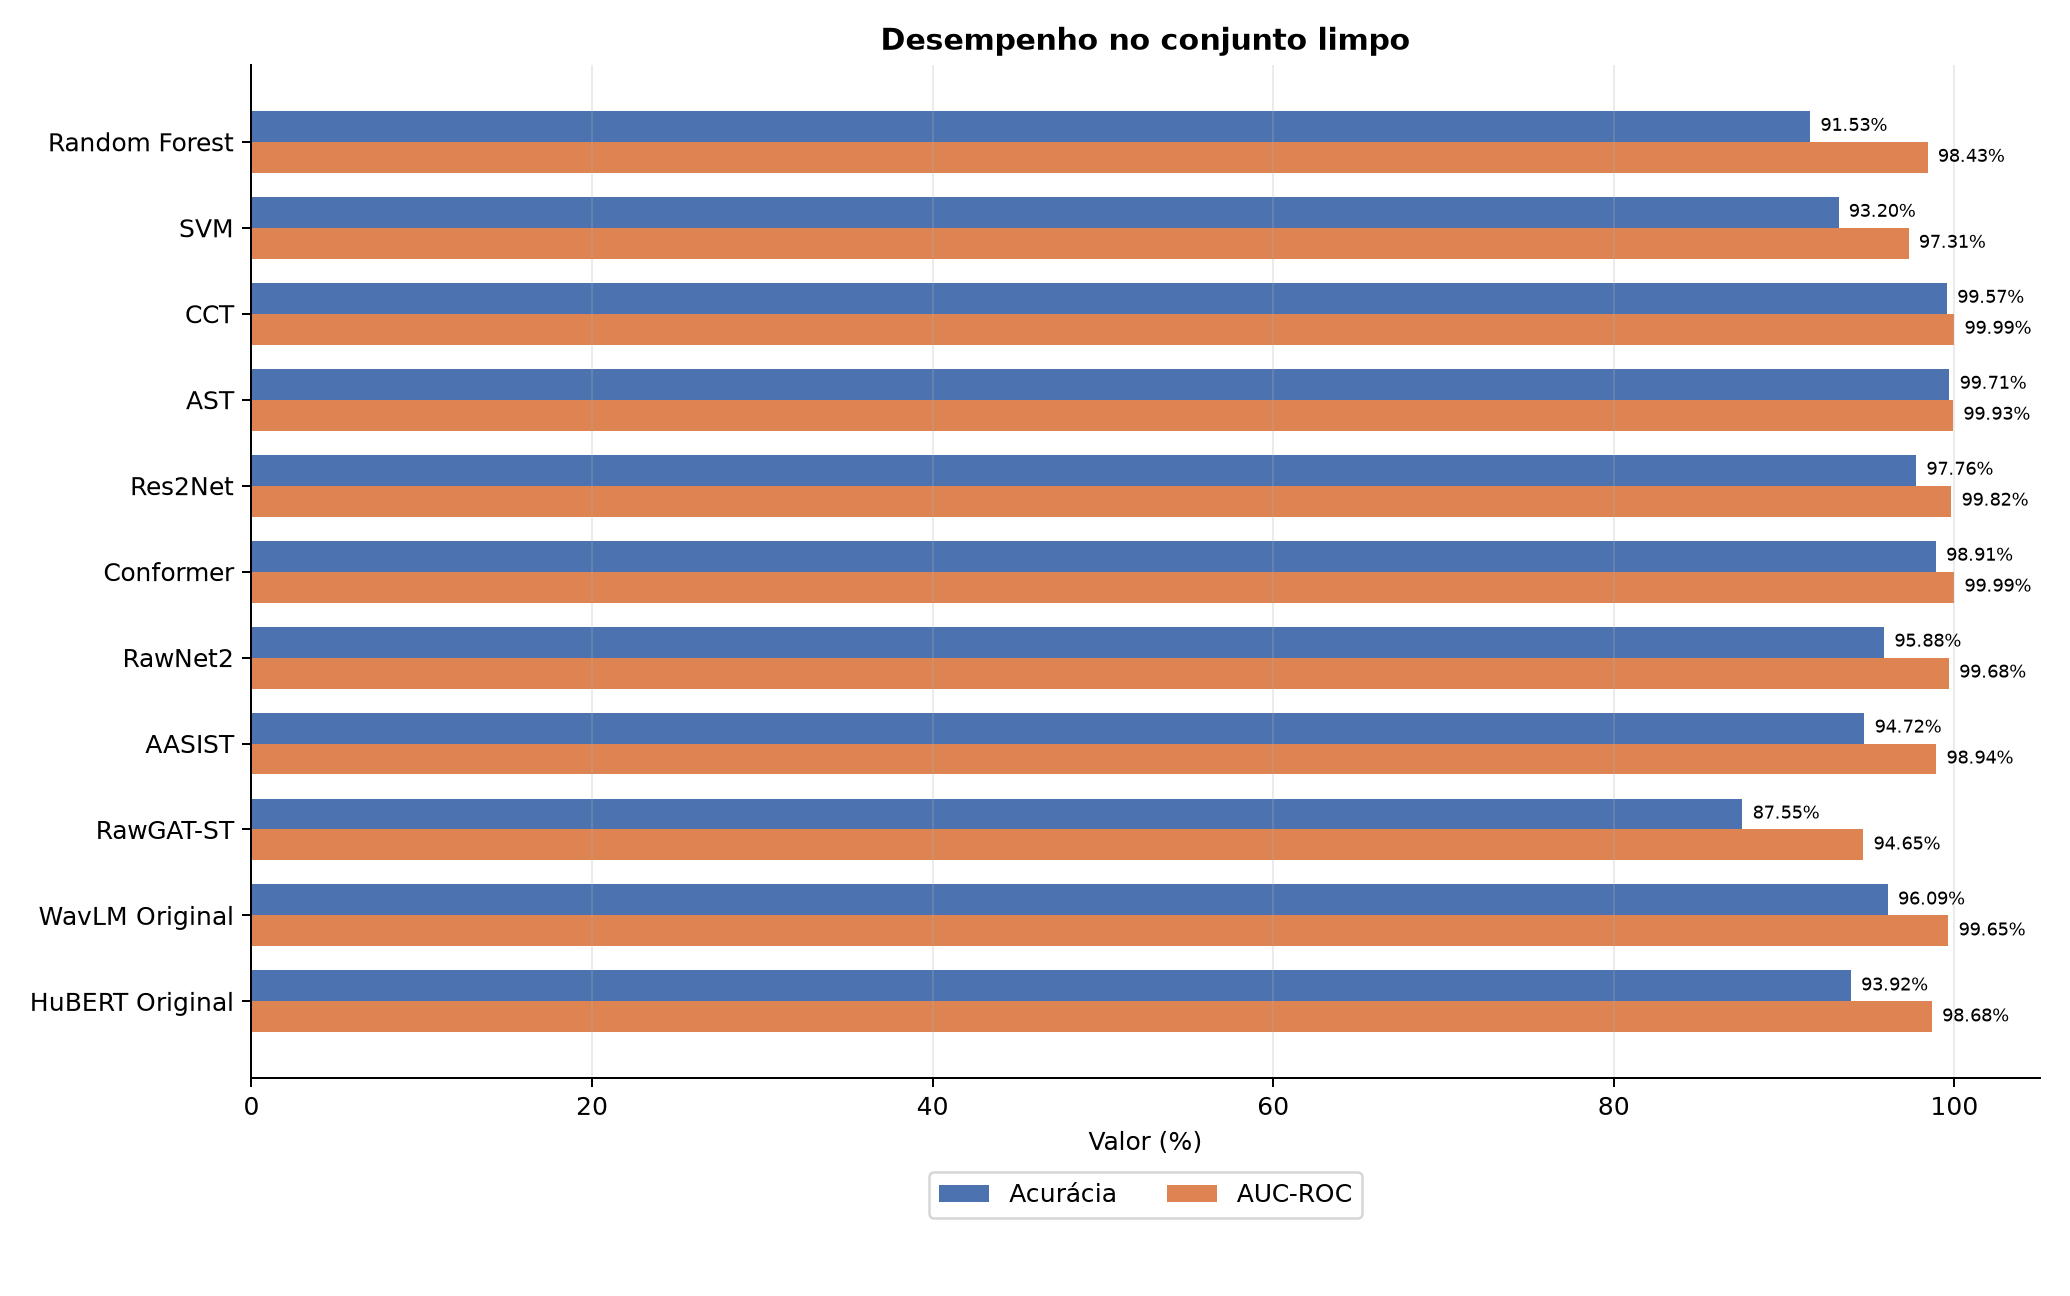
\includegraphics[width=\textwidth]{figures/benchmark_accuracy_auc.png}
\caption{Acurácia e AUC-ROC no conjunto de teste limpo.}
\label{fig:benchmark_accuracy_auc}
\end{figure}

\begin{figure}[ht]\centering

\includegraphics[width=\textwidth]{figures/benchmark_robustness.png}
\caption{Robustez a AWGN na forma de onda (acurácia vs.\ SNR).}
\label{fig:benchmark_robustness}
\end{figure}

\begin{figure}[ht]\centering

\includegraphics[width=0.92\textwidth]{figures/benchmark_eer.png}
\caption{Taxa de Erro Igual (EER) por arquitetura.}
\label{fig:benchmark_eer}
\end{figure}

\begin{figure}[ht]\centering

\includegraphics[width=0.92\textwidth]{figures/benchmark_tdcf.png}
\caption{$t$-DCF$^\ast$ por arquitetura.}
\label{fig:benchmark_tdcf}
\end{figure}

\begin{figure}[ht]\centering
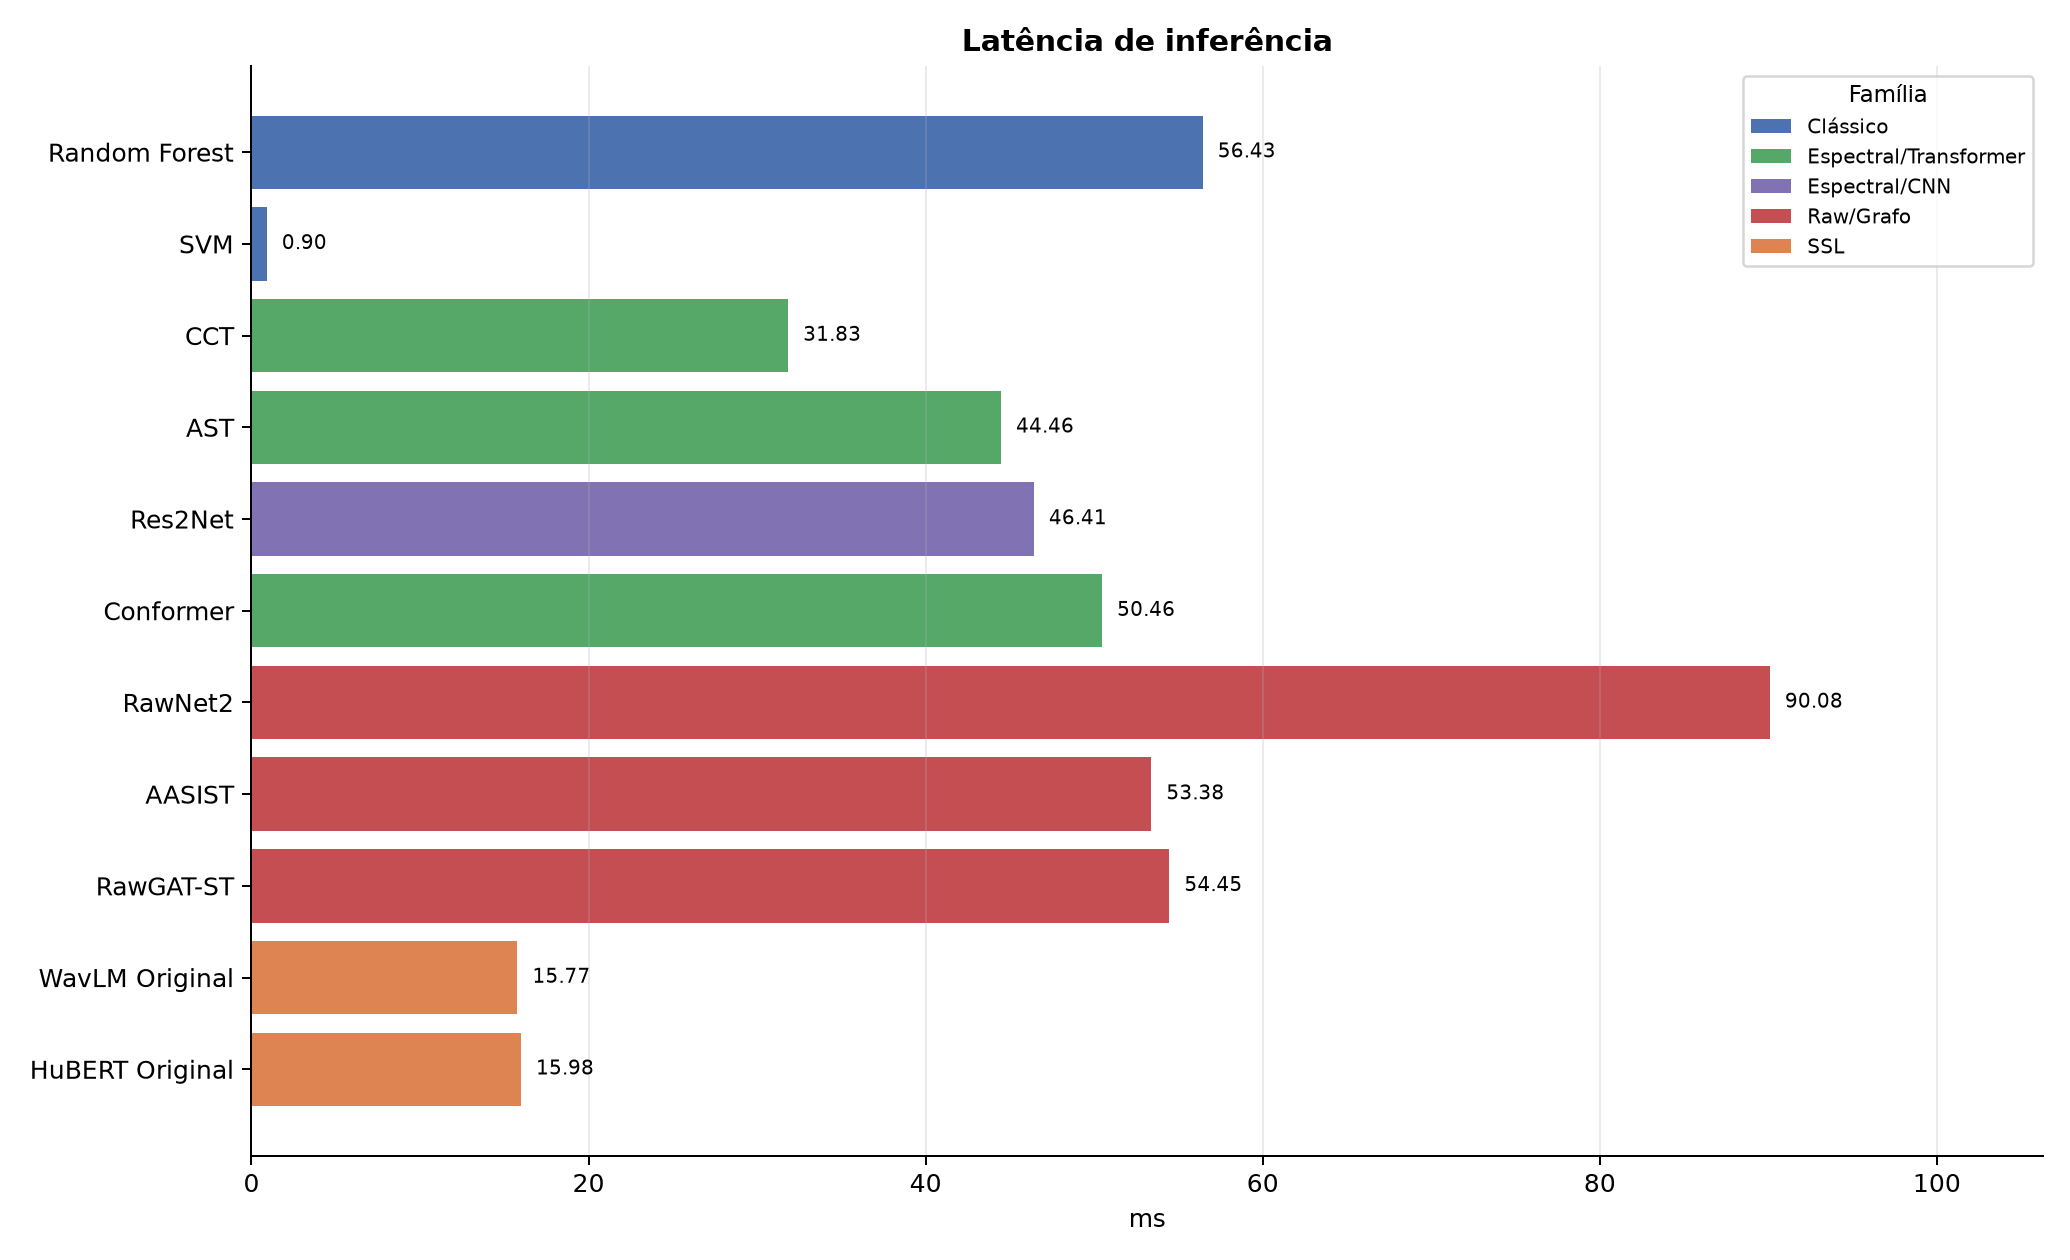
\includegraphics[width=0.95\textwidth]{figures/benchmark_latency.png}
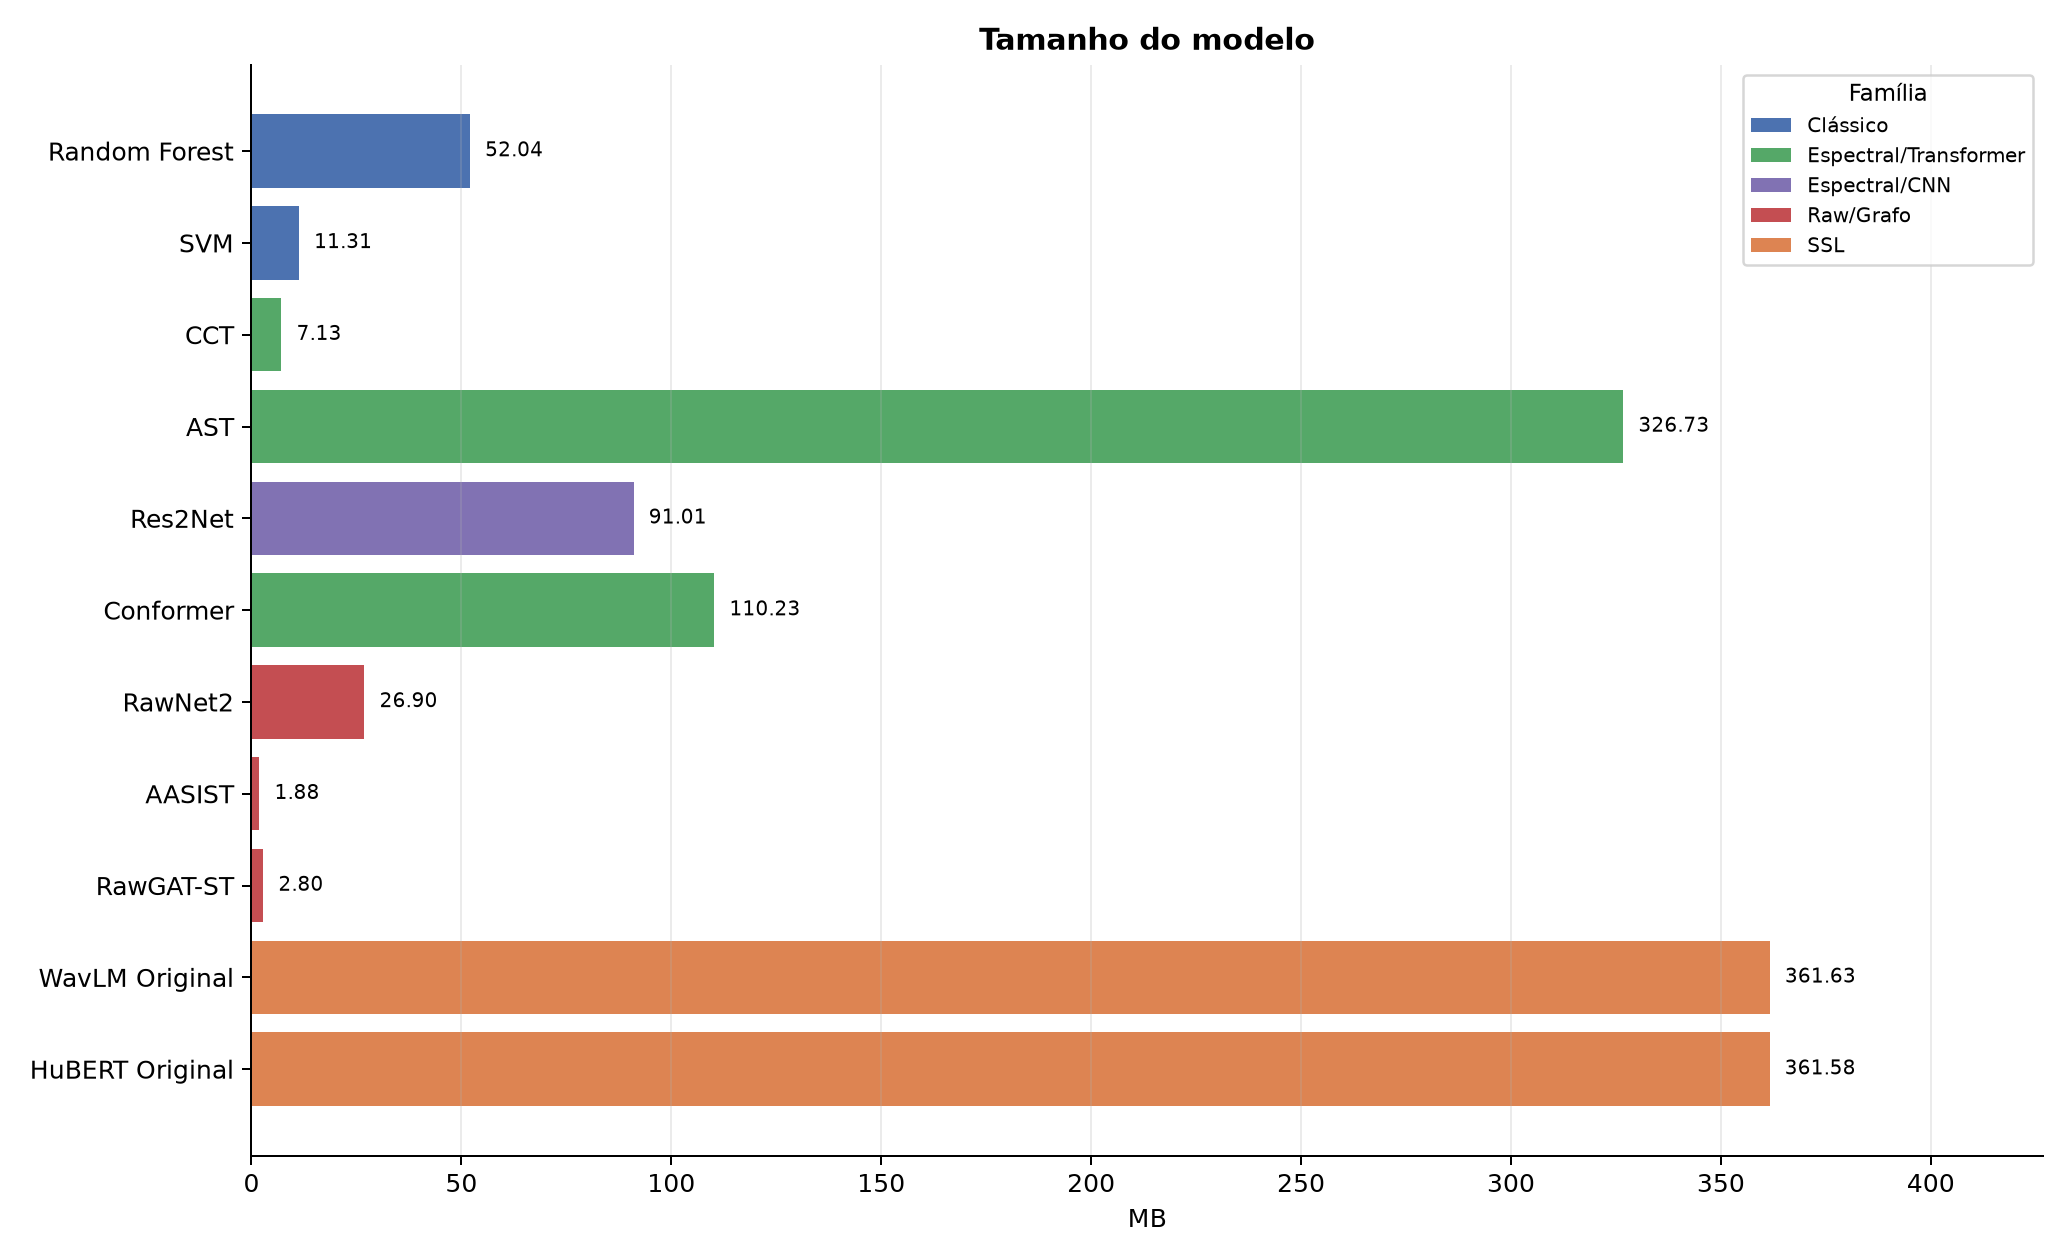
\includegraphics[width=0.95\textwidth]{figures/benchmark_size.png}
\caption{Latência e tamanho dos modelos.}
\label{fig:benchmark_latency_size}
\end{figure}

\begin{figure}[ht]\centering
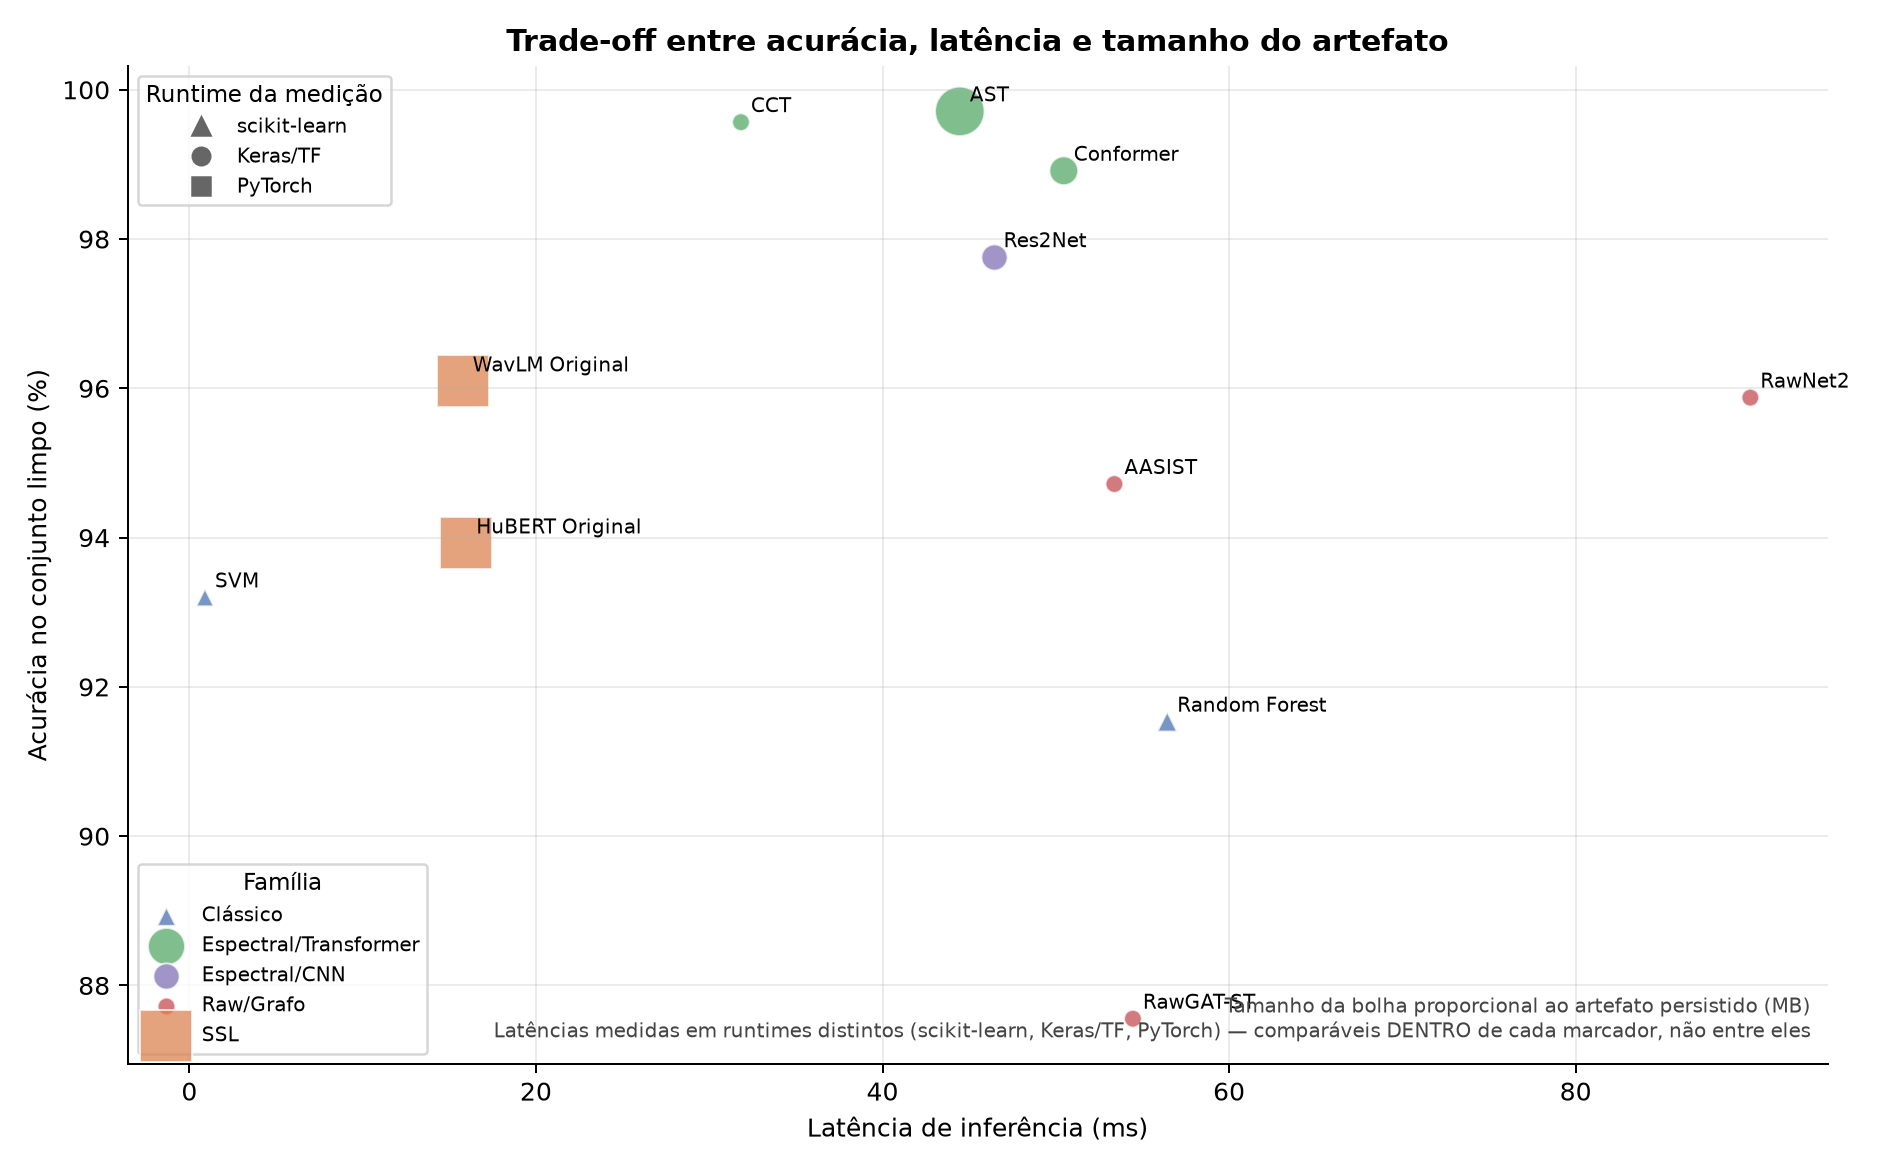
\includegraphics[width=0.95\textwidth]{figures/benchmark_accuracy_latency_tradeoff.png}
\caption{Trade-off entre acurácia, latência e tamanho dos artefatos.}
\label{fig:benchmark_accuracy_latency_tradeoff}
\end{figure}

\begin{figure}[ht]\centering
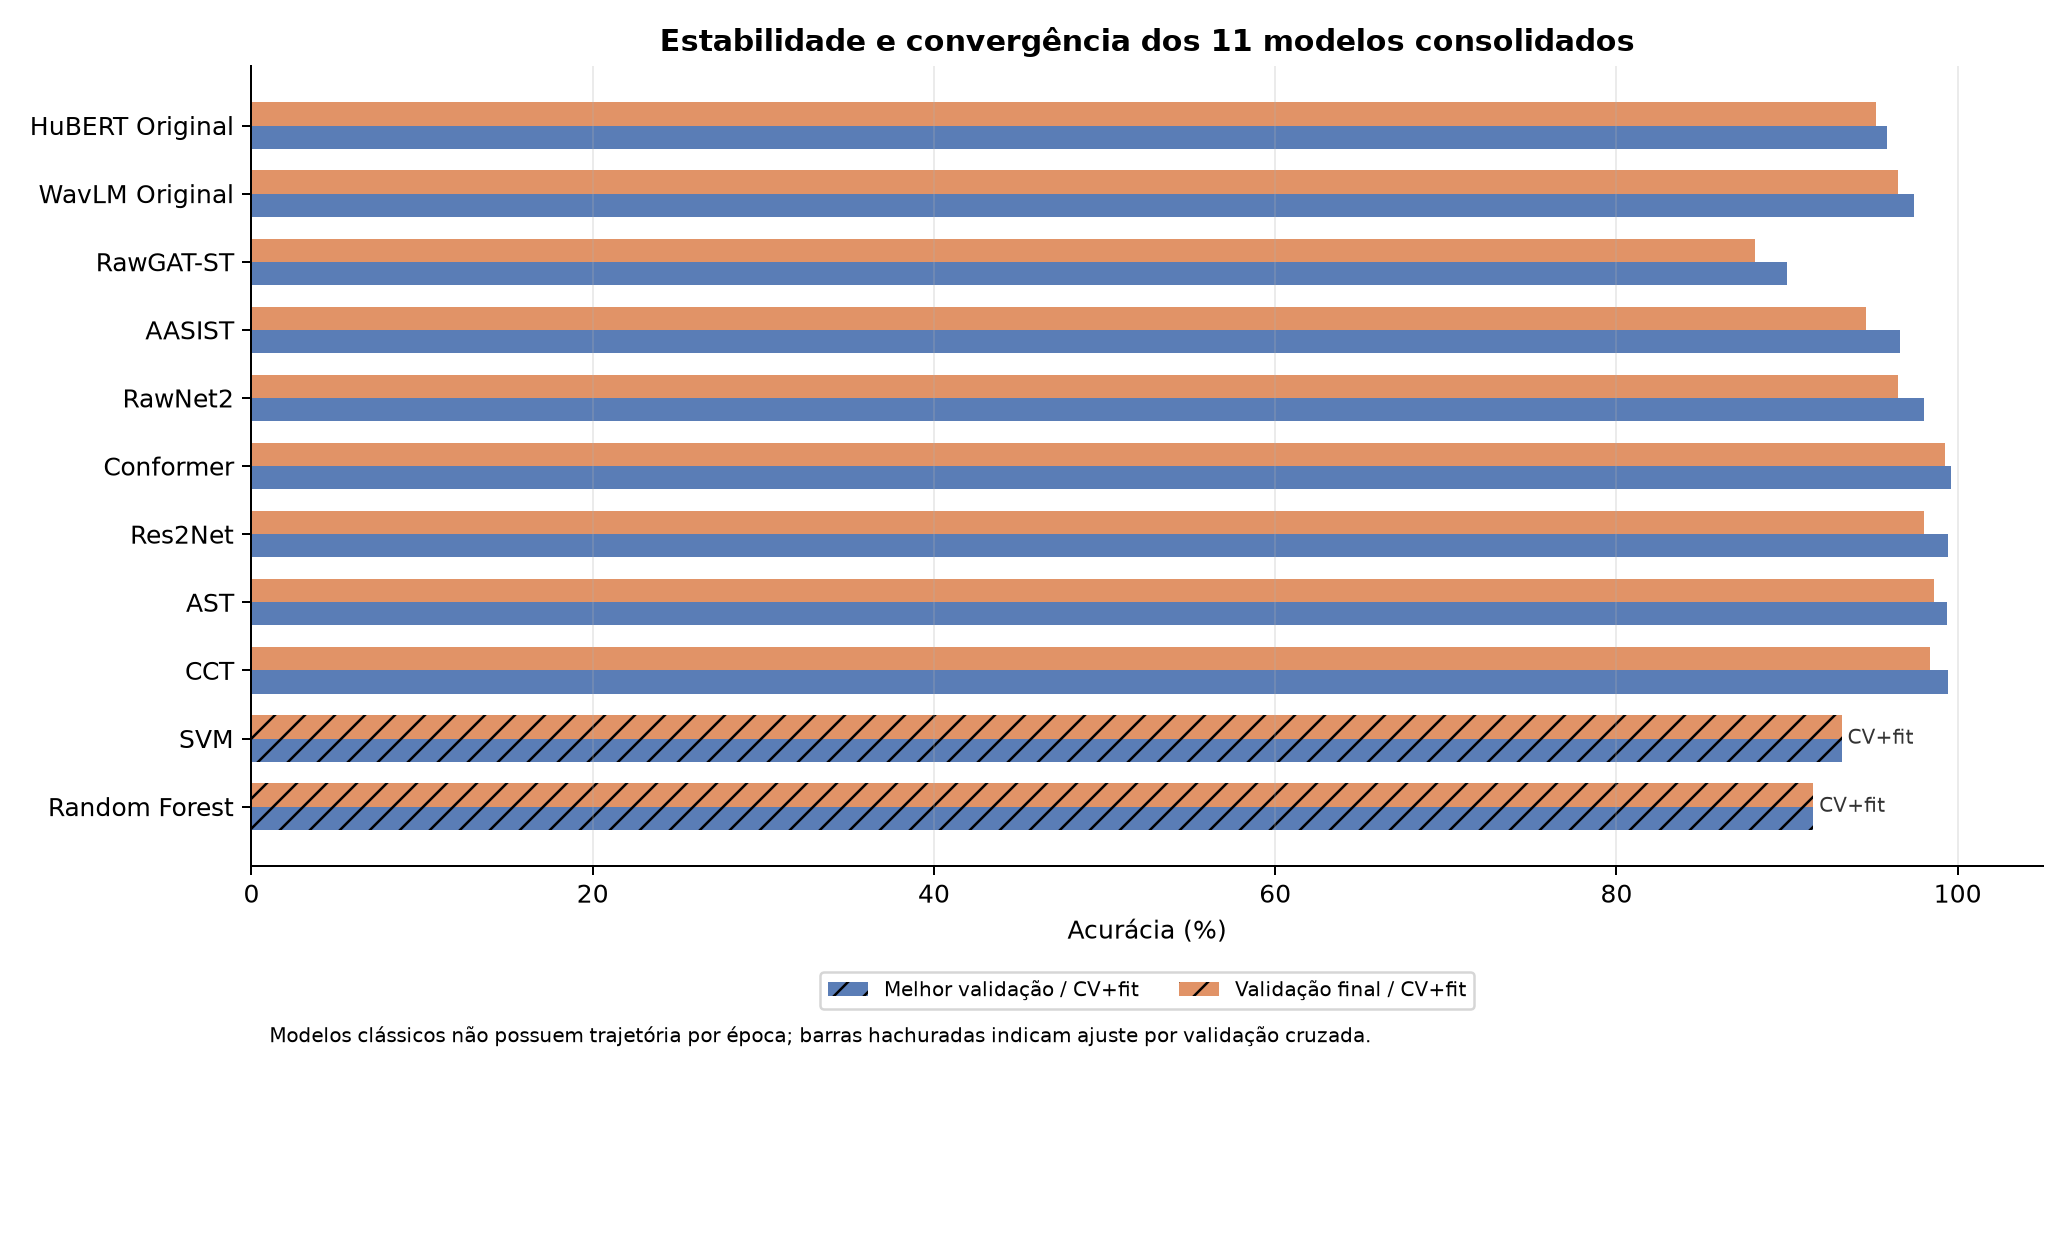
\includegraphics[width=0.95\textwidth]{figures/training_stability.png}
\caption{Resumo descritivo das curvas de validação em execução única; a diferença pico--final não demonstra, isoladamente, estabilidade de otimização. Modelos clássicos não possuem trajetória por época.}
\label{fig:training_stability}
\end{figure}

\begin{figure}[ht]\centering
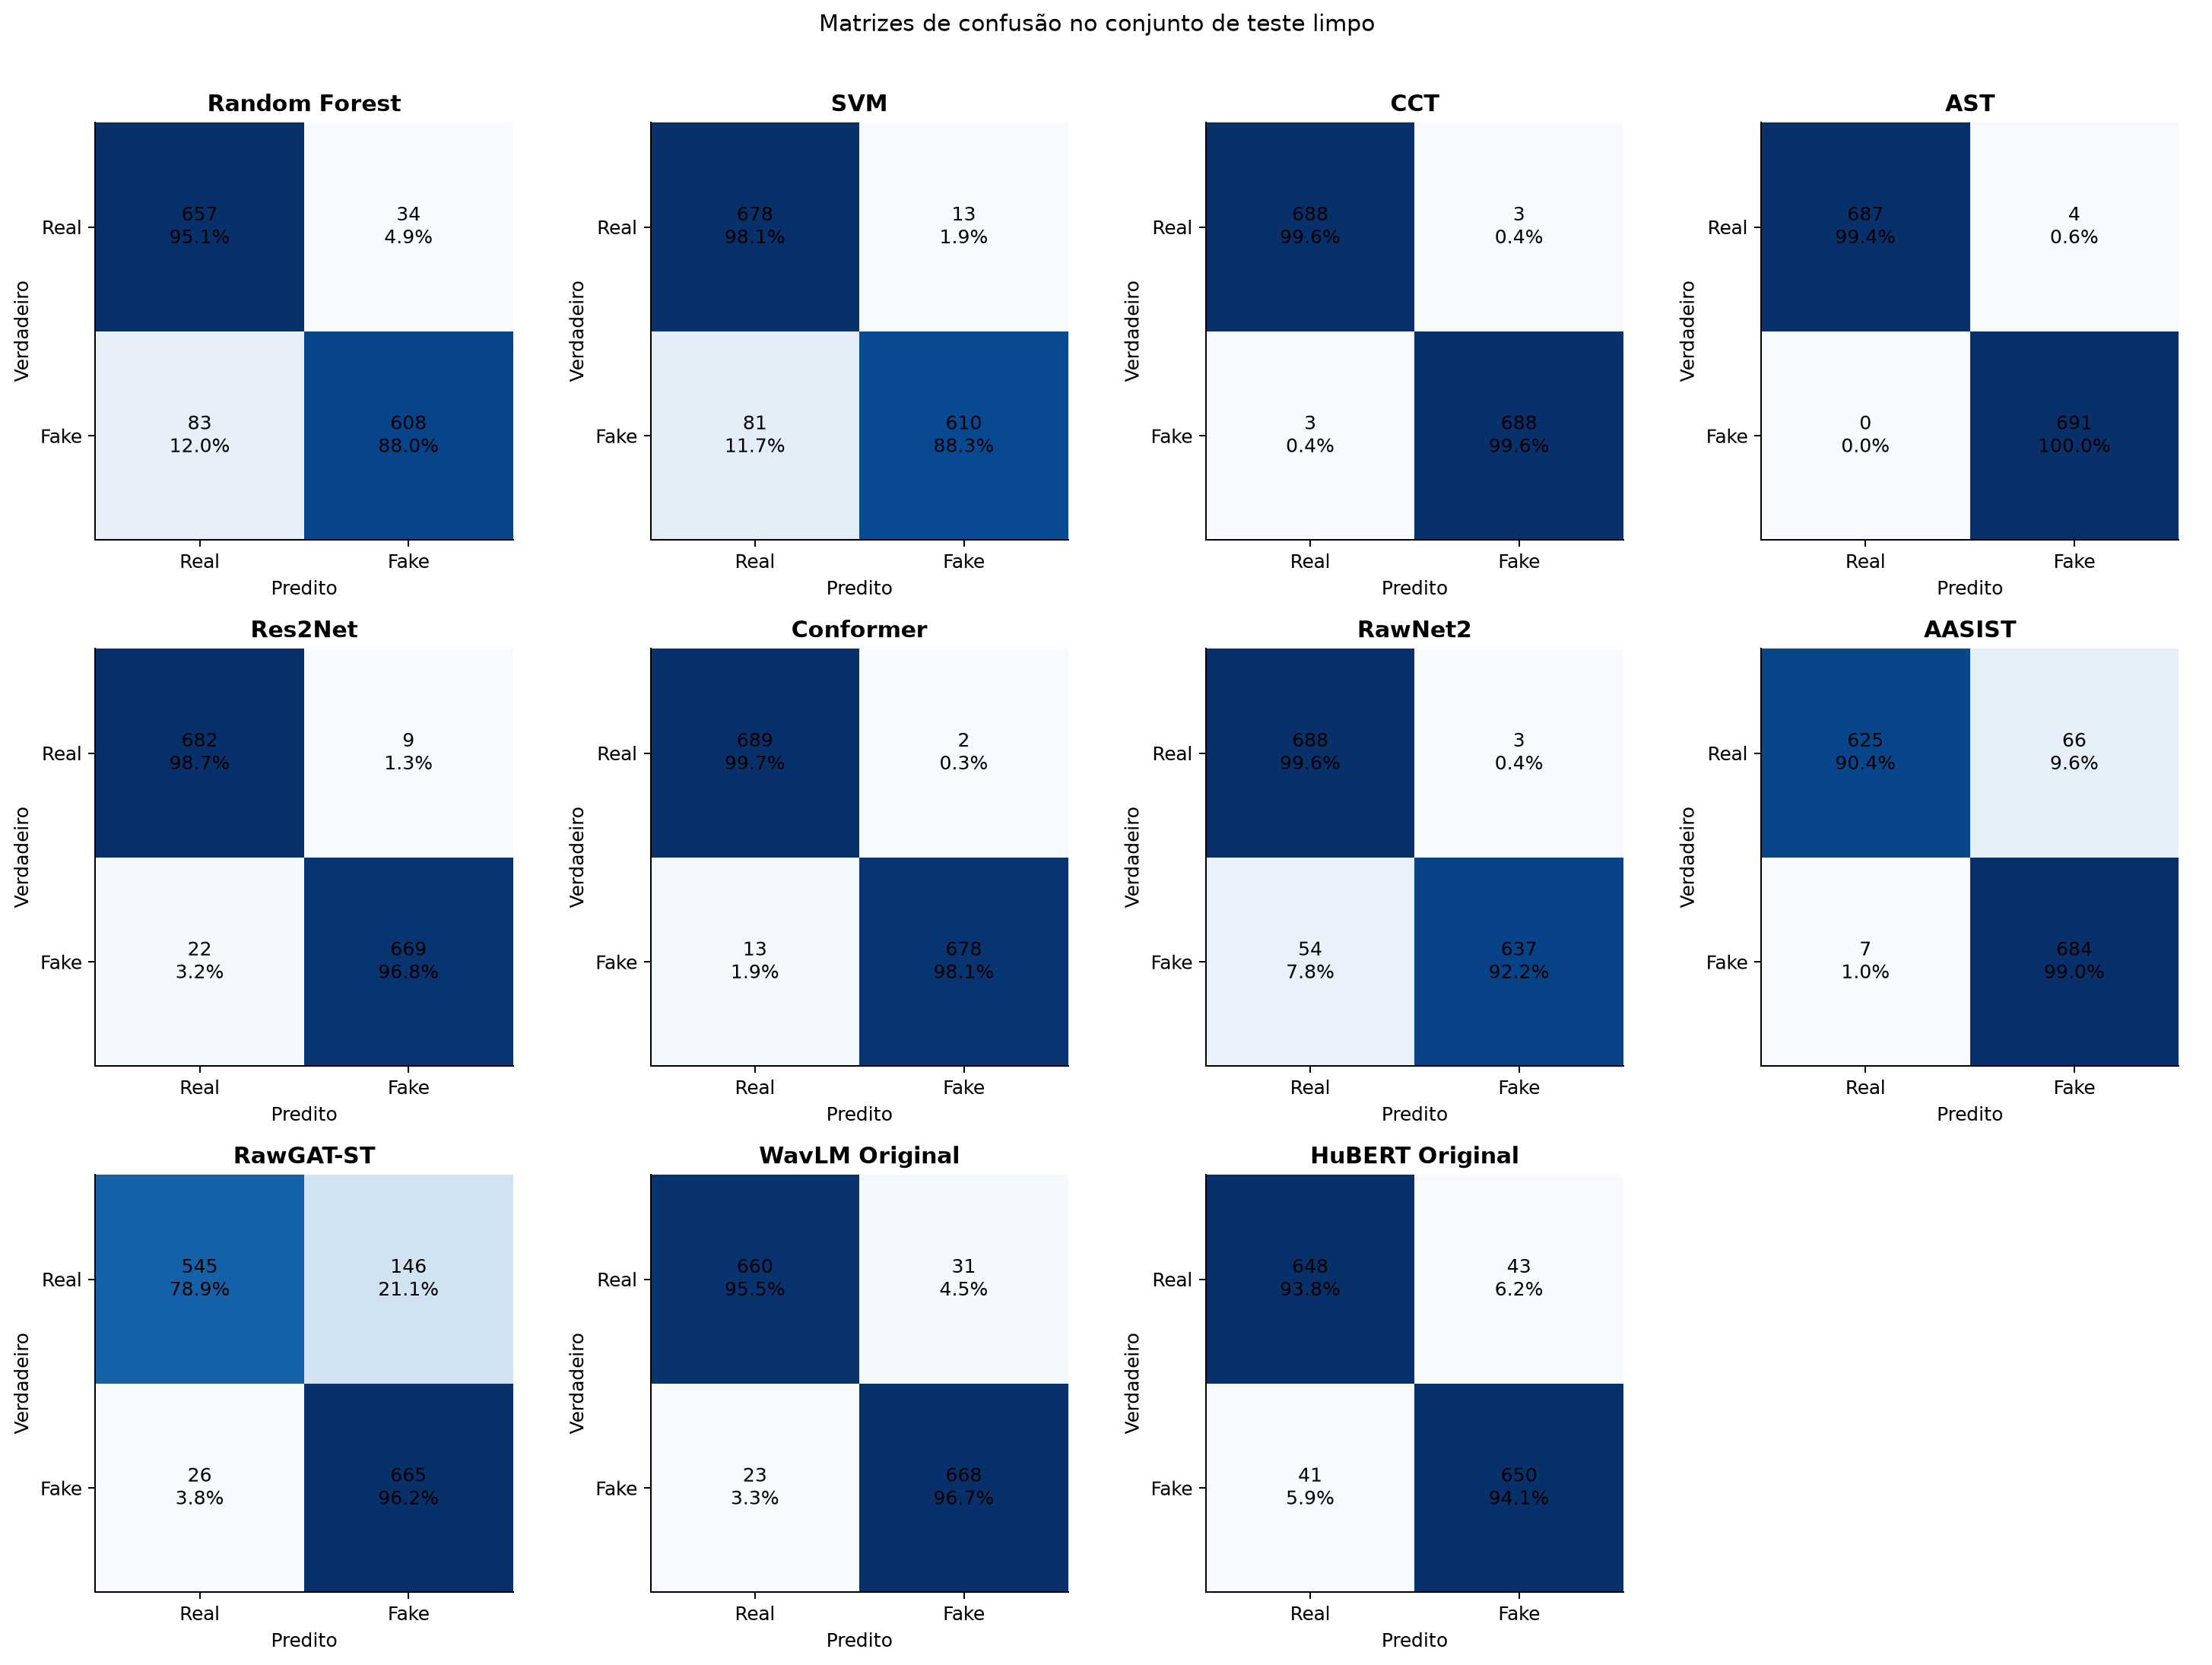
\includegraphics[width=\textwidth]{figures/confusion_matrices_article.png}
\caption{Matrizes de confusão dos onze modelos avaliados no artigo.}
\label{fig:confusion_matrices_article}
\end{figure}


\noindent\footnotesize{Nota sobre latência: mediana de \num{30} inferências de
amostra única (duas execuções de aquecimento), medida no ambiente de execução
de cada modelo --- GPU (RTX 3060) para os sete modelos Keras e os dois SSL em
PyTorch; CPU para SVM e Random Forest em scikit-learn. Os valores não são,
portanto, diretamente comparáveis entre \textit{runtimes}
(Seção~\ref{sec:ambiente_experimental}).}\normalsize

\subsection{Análise dos Resultados}
\label{sec:analise_resultados}

\subsubsection{Desempenho no Conjunto Limpo}

O recorte consolidado da Tabela~\ref{tab:resultados_consolidados} e da
Figura~\ref{fig:benchmark_accuracy_auc} mostra maior desempenho para AST e
CCT, com \num{99,71}\% e \num{99,57}\% de acurácia no conjunto de teste
limpo (EER de \num{0,14}\% e \num{0,43}\%). Em seguida aparecem Conformer
(\num{98,91}\%, EER de \num{0,29}\%) e Res2Net (\num{97,76}\%, EER de
\num{2,17}\%), indicando que redes neurais profundas extraem padrões
discriminativos relevantes no cenário experimental controlado
(QP1). Com \num[group-minimum-digits=4]{1382} amostras de teste, uma acurácia de \num{99,71}\%
corresponde a apenas \num{4} amostras mal classificadas, e a diferença entre
AST e CCT equivale a duas amostras. AST, CCT e Conformer devem, portanto, ser
tratados como \textbf{empate técnico}, e não como ordenamento estrito entre os
três primeiros colocados. Os testes pareados confirmam essa leitura. O McNemar
por \textit{cluster} (frase, \num{183} unidades) devolve, após correção de
Holm sobre as \num{55} comparações, $p = 1{,}00$ para AST\,$\times$\,CCT,
$p = 0{,}37$ para CCT\,$\times$\,Conformer e $p = 0{,}10$ para
AST\,$\times$\,Conformer --- nenhum significativo a \num{5}\%. O
\textit{bootstrap} pareado da diferença de EER é ainda mais claro: os três
intervalos de confiança de \num{95}\% contêm o zero
($\Delta\text{EER} = +0{,}29$ p.p., IC \num{95}\% $[-0{,}30; +0{,}64]$ para
AST\,$\times$\,CCT), com $p$ ajustado igual a $1{,}00$ nos três pares. O par
Res2Net--Conformer também não se separa pelo McNemar ($p = 0{,}18$), embora o
\textit{bootstrap} pareado de EER o distinga.

Cabe registrar o piso de resolução dos testes: com \num{5000} reamostragens e
\num{55} comparações, o menor $p$ corrigido por Holm que o procedimento
consegue expressar é $0{,}022$. Os pares reportados adiante com $p = 0{,}022$
estão \emph{nesse piso} --- a evidência é tão forte quanto o número de
reamostragens permite afirmar, e não uma medida pontual naquele valor.

A escolha da unidade de agrupamento também importa, e o protocolo reporta as
duas. Agrupando por \textbf{frase} (\num{183} unidades), \num{40} dos \num{55}
pares se separam pelo McNemar; agrupando por \textbf{locutor} (\num{11}
unidades) --- a unidade que corresponde à alegação de disjunção de locutores
e, por ser muito menor, bastante mais conservadora ---, apenas \num{17} se
separam. A conclusão sobre o topo do recorte, porém, é idêntica nas duas
leituras: AST, CCT e Conformer permanecem mutuamente indistinguíveis. Sob a
unidade locutor os três pares vão a $p = 1{,}00$; sob a unidade frase, mais
sensível por ter dezesseis vezes mais unidades, nenhum dos três alcança
significância a \num{5}\% após a correção de Holm --- $p = 1{,}00$,
$0{,}37$ e $0{,}10$, os valores reportados acima. O empate técnico no topo não
é, portanto, artefato da unidade de agregação escolhida.

Esse ordenamento contraria em parte a hierarquia sugerida pela
Tabela~\ref{tab:survey_geracoes}. Os \textit{backbones} SSL WavLM e HuBERT
(4\textordfeminine\ geração), avaliados com \textit{backbone} congelado, soma
ponderada das \num{13} camadas ocultas e \textit{pooling} média$\oplus$desvio
sobre a janela canônica de \SI{3}{\second} (Seção~\ref{subsec:ssl_raw}), ficam
na \textbf{metade inferior} do recorte --- \num{7}.\textordmasculine\ e
\num{8}.\textordmasculine\ lugares em EER (\num{3,62}\% e \num{5,93}\%),
abaixo de todas as arquiteturas espectrais e do RawNet2. A discussão desse
contraste com a literatura recente está na Seção~\ref{sec:conclusao}.

\subsubsection{A Previsão sobre Artefatos de Fase não se Confirma}

O ordenamento também permite fechar a previsão formulada na
Seção~\ref{sec:tecnologias_sintese}: se os artefatos de reconstrução de fase
fossem determinantes, e se de fato fossem inacessíveis a uma representação de
magnitude, as três arquiteturas de forma de onda deveriam liderar. Ocorre o
contrário. RawNet2, AASIST e RawGAT-ST ocupam a \num{6}.\textordfeminine, a
\num{7}.\textordfeminine\ e a \num{11}.\textordfeminine\ posições em acurácia
limpa, atrás de \emph{todas} as redes espectrais, que operam sobre mapas Mel de
magnitude e portanto não têm acesso à fase.

A previsão, portanto, \textbf{não se sustenta neste \textit{corpus}}, e há duas
leituras compatíveis com o observado. A primeira é que os clones XTTS-v2 deixam
vestígio dominante na \emph{envoltória} espectral e na dinâmica de amplitude ---
o segundo e o terceiro casos daquela lista ---, e não na fase; a análise de
importância do vetor tabular reforça essa leitura, ao encontrar estatísticas de
amplitude e coeficientes LFCC como fatores dominantes. A segunda é que o acesso
à fase não basta: dispor da forma de onda é condição necessária, não suficiente,
para explorar inconsistências de fase, e nada garante que o treinamento conduza
a rede a aprendê-las quando um atalho mais simples está disponível na
envoltória.

Distinguir as duas exigiria um ensaio de ablação --- por exemplo, avaliar as
redes de forma de onda sobre sinais com fase deliberadamente randomizada e
verificar quanto do desempenho sobrevive. O recorte atual não o permite, e a
questão fica em aberto (Seção~\ref{sec:trabalhos_futuros}).

O modelo mais fraco do conjunto é o \textbf{RawGAT-ST}, com EER de
\num{11,87}\% e min $t$-DCF$^\ast$ de \num{0,3149} --- o único que os testes
pareados separam de \emph{todos} os outros dez, com significância após correção
de Holm. O AASIST, ao contrário do que a proximidade arquitetural sugeriria,
registra EER de \num{2,60}\% e ocupa a \num{5}.\textordfeminine\ posição,
à frente de RawNet2, dos dois SSL e dos dois classificadores clássicos.

Os valores de AASIST e RawGAT-ST ficam acima dos reportados pelos artigos
originais no ASVspoof 2019 LA --- EER de \num{0,83}\% para o AASIST~\cite{jung2022aasist}, \num{1,06}\% para o RawGAT-ST~\cite{tak2021rawgatst} e
$\approx$\num{1,1}\% para o RawNet2~\cite{tak2021rawnet2} ---, mas a distância
tem magnitudes muito diferentes nos dois casos: o AASIST fica a
\num{1,8}~p.p.\ do valor publicado, enquanto o RawGAT-ST fica a
\num{10,8}~p.p. Para o AASIST, a diferença é compatível com a mudança de
\textit{corpus} e de escopo; para o RawGAT-ST, ela indica um problema de
treinamento específico deste protocolo, discutido na análise de estabilidade
adiante. As implementações de ambos são variantes alinhadas aos artigos, não
réplicas exatas, e o \textit{corpus} deste trabalho --- em português, com um
único gerador --- é distinto e mais restrito que o ASVspoof, que combina
dezenas de sistemas de ataque. A hierarquia observada é, portanto, específica
deste protocolo e não constitui refutação dos resultados publicados para essas
arquiteturas.

A decomposição dos erros por tipo
(Figura~\ref{fig:confusion_matrices_article}) revela padrões operacionalmente
distintos, que a acurácia agregada esconde. O AST erra \num{4} amostras no
total, \textbf{todas falsos positivos}: no limiar fixo de $0{,}5$ ele não
aceitou nenhum \textit{spoof} --- o comportamento mais favorável possível no
cenário de biometria em \textit{tandem}. O CCT distribui seus \num{6} erros
simetricamente (\num{3} contra \num{3}).

AASIST e RawGAT-ST concentram os erros em falsos positivos (AASIST: \num{66}
amostras \textit{bonafide} rejeitadas contra \num{7} \textit{spoofs} aceitos;
RawGAT-ST: \num{146} contra \num{26}), o que penaliza a usabilidade pela
rejeição indevida de usuários legítimos, mas preserva a segurança. O padrão
oposto --- e mais crítico --- aparece em RawNet2 (\num{54} \textit{spoofs}
aceitos contra \num{3} rejeições indevidas), SVM (\num{81} contra \num{13}),
\textit{Random Forest} (\num{83} contra \num{34}) e, em menor grau, Conformer
(\num{13} contra \num{2}): aceitar um ataque custa mais do que rejeitar um
usuário genuíno ($C_{\text{fa}} = 10 \gg C_{\text{miss}} = 1$;
Seção~\ref{sec:tdcf_def}), e é esse desequilíbrio que o
min $t$-DCF$^\ast$ penaliza adiante.

\subsubsection{Importância de Características no Vetor Tabular}

A Figura~\ref{fig:rf_feature_importance} apresenta a importância \textbf{por
permutação} das características do vetor tabular de \num{183} descritores
(Seção~\ref{sec:caracteristicas}), medida sobre a partição de teste com
\num{30} repetições por característica
(\path{scripts/reporting/export_rf_feature_importance.py}). A escolha do
método é deliberada: a redução média de impureza (MDI, ou ``importância de
Gini'') é enviesada a favor de variáveis contínuas e de alta cardinalidade, e
por isso não é usada na análise confirmatória --- a importância por permutação
mede a queda real de acurácia quando a característica é destruída, que é a
grandeza de interesse.

Agregando por família, o resultado contraria a expectativa de domínio cepstral:
as \textbf{estatísticas temporais} concentram \num{44,7}\% da importância
total, seguidas de perto pelos coeficientes \textbf{LFCC} (\num{41,6}\%),
com MFCC (\num{8,7}\%) e RASTA-PLP (\num{5,0}\%) bem atrás. Individualmente, o
descritor mais informativo é o \textbf{desvio-padrão} da forma de onda
(\num{21,5}\% sozinho), seguido da média (\num{10,9}\%) e do LFCC20 médio
(\num{5,9}\%). Entre as \num{15} características mais importantes, \num{5} são
temporais, \num{7} são LFCC e \num{3} são MFCC.

Os percentuais acima normalizam sobre a soma das importâncias \textbf{truncadas
em zero}. O truncamento não é cosmético e precisa ser declarado: \num{59} das
\num{183} características têm importância por permutação negativa --- o que
significa que embaralhá-las \emph{melhorou} a acurácia, um artefato de ruído
amostral sem interpretação causal. Sob a normalização bruta, que soma também
esses valores, o quadro se desloca: temporais passam a \num{51,0}\%, LFCC a
\num{36,7}\%, MFCC a \num{6,8}\% e RASTA-PLP a \num{5,5}\%. A leitura
qualitativa --- domínio das estatísticas de amplitude, LFCC bem à frente do
MFCC --- é a mesma nas duas; a repartição exata entre os blocos temporal e
cepstral, não.

Duas leituras seguem daí. Primeiro, a predominância de estatísticas de
amplitude sugere que parte do poder discriminativo do vetor tabular vem de
diferenças de \emph{envelope e dinâmica} entre fala natural e sintetizada ---
não de estrutura espectral fina. Segundo, o peso do LFCC ante o MFCC é
consistente com a literatura de \textit{anti-spoofing}, que reporta o
espaçamento linear em frequência como mais sensível a artefatos de síntese do
que a escala Mel, desenhada para percepção. Esse contraste é coerente com a
extensão do vetor de \num{63} para \num{183} descritores; note-se, porém, que
ele \emph{não} a valida de forma independente, já que a extensão foi decidida
com conhecimento do comportamento no teste e a importância aqui é medida na
mesma partição (Seção~\ref{sec:caracteristicas}).

\begin{figure}[htbp]
\centering
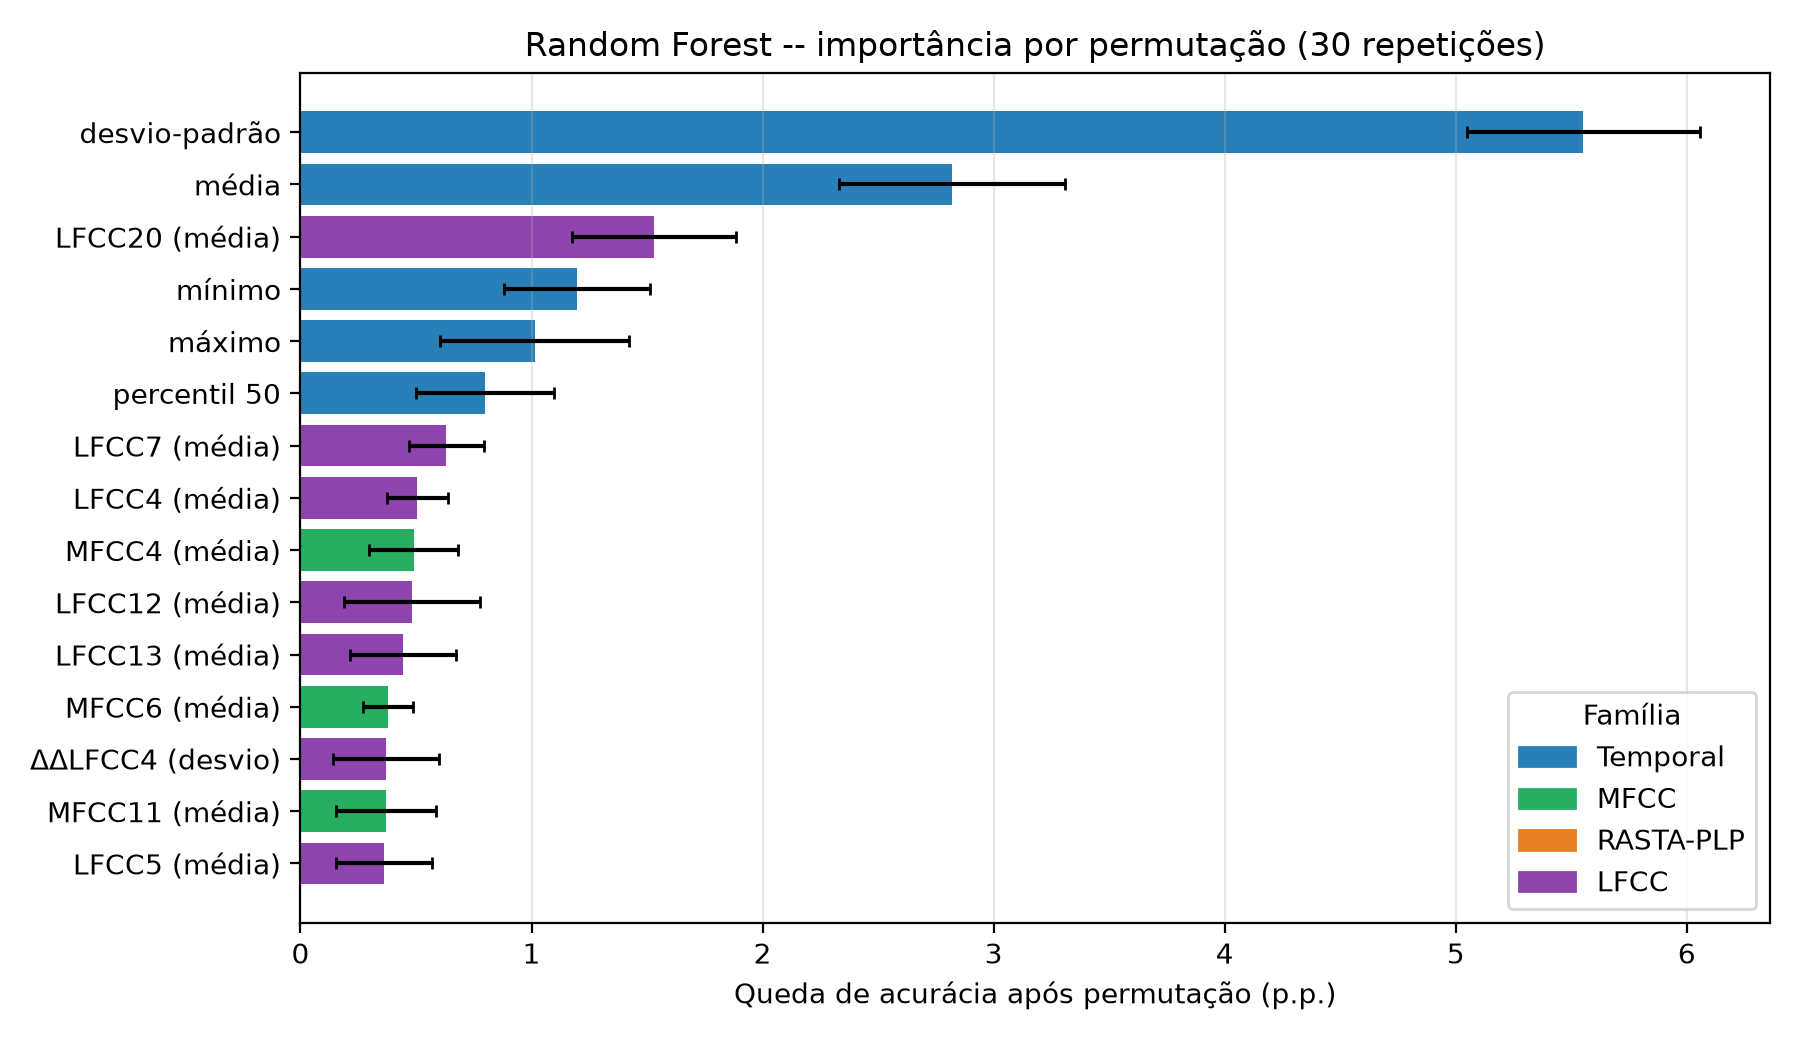
\includegraphics[width=0.92\textwidth]{figures/rf_feature_importance.png}
\caption{Importância por permutação das \num{15} características mais
relevantes do \textit{Random Forest}, coloridas por família (temporal, LFCC,
MFCC, RASTA-PLP), medida na partição de teste com \num{30} repetições.
Agregadas, as famílias respondem por \num{44,7}\% (temporal), \num{41,6}\%
(LFCC), \num{8,7}\% (MFCC) e \num{5,0}\% (RASTA-PLP) da importância total.}
\label{fig:rf_feature_importance}
\end{figure}

Vale notar a tensão com a leitura clássica da literatura de
\textit{anti-spoofing} de primeira geração~\cite{sahidullah2015comparison},
que atribui à envoltória cepstral o grosso da informação discriminativa. Aqui,
somando LFCC e MFCC, o bloco cepstral responde por \num{50,3}\% sob a
normalização truncada (\num{43,5}\% sob a bruta) --- em torno de metade da
importância, mas dividindo espaço com estatísticas de amplitude que
aquela literatura trata como secundárias. Uma explicação plausível é o
pareamento: com texto e locutor constantes entre as classes, diferenças de
conteúdo que normalmente dominariam a variância cepstral desaparecem, e o que
resta são as assinaturas do sintetizador --- entre elas, a compressão de faixa
dinâmica característica de \textit{vocoders} neurais.

Independentemente da família, o \textit{Random Forest} é um dos modelos menos
robustos sob ruído (Tabela~\ref{tab:robustez_awgn}), o que reforça que a
fragilidade dos clássicos decorre da natureza \emph{agregada} do vetor ---
médias e desvios globais por amostra descartam a estrutura tempo-frequência
fina que as redes espectrais exploram --- e não da ausência de características
apropriadas.

\subsubsection{Robustez a Ruído: o Achado Central}

A Tabela~\ref{tab:robustez_awgn} e a Figura~\ref{fig:benchmark_robustness}
mostram degradação suave e majoritariamente monotônica sob o protocolo
\textit{waveform}-AWGN (ruído aplicado à forma de onda antes de qualquer
\textit{frontend}, com exemplos ruidosos compatíveis também no treino). Duas
exceções merecem registro, e ambas decorrem do casamento entre treino e
avaliação: AASIST e RawGAT-ST \emph{melhoram} ligeiramente a
\SI{30}{\decibel} em relação ao conjunto limpo (\num{94,72} $\rightarrow$
\num{95,01}\% e \num{87,55} $\rightarrow$ \num{87,63}\%), porque metade dos
exemplos de ajuste é ruidosa e o limpo passa a ser, para esses dois modelos, a
condição menos representada. O RawGAT-ST ainda inverte entre \num{10} e
\SI{5}{\decibel} (\num{77,21} contra \num{77,64}\%), o que é coerente com a sua
instabilidade de treino e com o intervalo amostral de $\pm\num{2,2}$ pontos
nesse nível. O
ordenamento a \SI{10}{\decibel} \textbf{difere substancialmente} do observado
no conjunto limpo: lidera o Res2Net (\num{92,40}\%), seguido de AASIST
(\num{91,68}\%), Conformer (\num{91,46}\%), RawNet2 (\num{90,38}\%) e CCT
(\num{90,30}\%); depois vêm WavLM Original (\num{88,35}\%), AST
(\num{88,21}\%), HuBERT Original (\num{85,75}\%), SVM (\num{85,53}\%) e
\textit{Random Forest} (\num{82,71}\%); o RawGAT-ST fecha o conjunto com
\num{77,21}\% --- nenhum deles próximo do acaso (\num{50}\%).

A reorganização é o achado: os dois melhores modelos no limpo (AST e CCT) caem
para \num{7}.\textordfeminine\ e \num{5}.\textordfeminine\ posições sob ruído,
enquanto o AASIST sobe da \num{7}.\textordfeminine\ para a
\num{2}.\textordfeminine. Acurácia em condição limpa, isoladamente,
não prediz robustez.

\paragraph{Quanto dessa ordem é estatisticamente sustentável.} O aparato
pareado aplicado ao conjunto limpo foi estendido aos níveis ruidosos --- McNemar
por \textit{cluster} e \textit{bootstrap} pareado de EER, ambos com \num{5000}
reamostragens e correção de Holm sobre as \num{55} comparações --- e o veredito
exige cautela com a leitura do \textit{ranking}. A \SI{10}{\decibel} separam-se
\num{31} pares pelo McNemar e \num{32} pelo \textit{bootstrap} sob a unidade
frase; sob a unidade locutor, apenas \num{7} por ambos.

\textbf{Nenhum dos dez pares entre os cinco primeiros atinge significância por
nenhum dos dois testes.} Pelo McNemar, o menor $p$ ajustado do grupo é
$0{,}50$; pelo \textit{bootstrap}, $0{,}055$
(Conformer\,$\times$\,RawNet2) --- próximo do limiar, mas ainda acima dele.
Res2Net, AASIST, Conformer, RawNet2 e CCT formam, portanto, um \textbf{bloco
indistinguível} a \SI{10}{\decibel}, assim como AST, CCT e Conformer formam um
no conjunto limpo.

Isso não desfaz o achado; delimita-o. O que os dados sustentam é o
\emph{deslocamento entre blocos}, e não a ordem dentro deles: AST e CCT deixam o
bloco de topo do conjunto limpo, passando a integrá-lo (CCT) ou a ficar abaixo
dele (AST) sob ruído. No extremo oposto, o RawGAT-ST separa-se de
\num{10} dos \num{10} demais modelos pelo McNemar e de \num{9} pelo
\textit{bootstrap} de EER a \SI{10}{\decibel}. Afirmações do tipo ``o Res2Net
lidera a robustez'' devem ser lidas como ordenação amostral, não como diferença
demonstrada; a de que ``o RawGAT-ST é o menos robusto'' está estabelecida.

A \SI{5}{\decibel} o poder de resolução cai, como esperado da degradação mais
severa: separam-se \num{33} pares pelo McNemar e \num{36} pelo
\textit{bootstrap} sob a unidade frase (\num{14} e \num{10} por locutor), e o
próprio RawGAT-ST já não se distingue de todos --- apenas de \num{7} dos
\num{10}, por ambos os testes. Sob o SNR não visto, portanto, nem mesmo o pior
modelo do recorte é separável do conjunto com a confiança que \SI{10}{\decibel}
permite.

Dois achados emergem dessa leitura (QP2). Primeiro, o casamento entre o ruído
de treino e o de teste importa mais do que a família arquitetural: com
exemplos ruidosos compatíveis no treino, até os classificadores clássicos ---
limitados a um vetor de \num{183} descritores agregados --- degradam
suavemente (SVM: \num{93,20}\% $\rightarrow$ \num{85,53}\%; \textit{Random
Forest}: \num{91,53}\% $\rightarrow$ \num{82,71}\%), sem o colapso que se
observaria caso o ruído aparecesse apenas na avaliação.

Segundo, a fragilidade relativa \emph{não} se distribui por família
arquitetural, como se poderia supor. As duas redes de grafos sobre áudio bruto
se comportam de maneira oposta: o RawGAT-ST perde \num{10,3} pontos
percentuais entre o conjunto limpo e \SI{10}{\decibel} (\num{87,55}\%
$\rightarrow$ \num{77,21}\%), a menor robustez absoluta do recorte, enquanto o
AASIST --- mesma família, mesmo domínio de entrada, mesmo \textit{front-end}
SincNet --- degrada apenas \num{3,0} pontos (\num{94,72}\% $\rightarrow$
\num{91,68}\%) e termina como o \num{2}.\textordmasculine\ mais robusto. O
RawGAT-ST é também o único dos dois que apresenta sobreajuste e oscilação de
validação (Seção~\ref{sec:analise_resultados}, ``Estabilidade de Treinamento''),
o que torna o sobreajuste a explicação mais plausível para o contraste --- com
a ressalva, decisiva, de que se trata de \textbf{uma única comparação}.

Esse resultado \textbf{rejeita as duas hipóteses mais plausíveis} formuladas na
QP2 (Seção~\ref{sec:questoes_pesquisa}). A \emph{representação de entrada} não
explica a dissociação: AASIST e RawGAT-ST consomem a mesma forma de onda, pelo
mesmo \textit{front-end} SincConv, e separam-se por \num{14,5} pontos
percentuais a \SI{10}{\decibel}. A \emph{capacidade do modelo} tampouco: os dois
são os menores do recorte (\num{396312} e \num{650204} parâmetros), enquanto o
maior modelo treinado do zero --- o Conformer, com \num{28,6}~milhões --- fica
entre eles em robustez.

Seria tentador promover o sobreajuste a explicação geral, e a versão preliminar
desta análise o fez. \textbf{Os próprios dados não sustentam essa
generalização.} O diagnóstico automático classifica \emph{dois} modelos como
\path{unstable_oscillation}, e a Tabela~\ref{tab:instabilidade_robustez} mostra
que eles ocupam extremos opostos da robustez:

\begin{table}[H]
\centering
\caption{Os dois modelos diagnosticados como instáveis e sua posição na
robustez a \SI{10}{\decibel}. A instabilidade de validação, isoladamente, não
ordena o recorte.}
\label{tab:instabilidade_robustez}
\small\singlespacing
\begin{tabular}{@{}lccc@{}}
\toprule
\textbf{Modelo} & \textbf{Diagnóstico} & \textbf{Acur.\ a \SI{10}{\decibel}} & \textbf{Posição} \\
\midrule
Conformer  & \path{unstable_oscillation} & \num{91,46}\% & \num{3}.\textordfeminine \\
RawGAT-ST  & \path{unstable_oscillation} & \num{77,21}\% & \num{11}.\textordfeminine \\
\bottomrule
\end{tabular}
\end{table}

\noindent
O Conformer é instável pelo mesmo critério e, ainda assim, é o
\num{3}.\textordmasculine\ mais robusto do conjunto, à frente de seis modelos
classificados como estáveis. A variável ``estabilidade de validação'' tem, neste
recorte, duas observações positivas --- e uma delas é contraexemplo direto.

A conclusão honesta da QP2 é, portanto, \textbf{negativa em três frentes}:
nem a representação de entrada, nem a capacidade do modelo, nem o diagnóstico
automático de estabilidade ordenam a robustez a ruído. O contraste
AASIST\,$\times$\,RawGAT-ST permanece a observação mais sugestiva do recorte, e
o sobreajuste é a leitura mais econômica para ele, mas com $n = 2$ ela é
\emph{hipótese para trabalho futuro}, não achado estabelecido. Separá-la de
alternativas --- inicialização infeliz, interação entre a construção dinâmica
dos grafos e o regime de ruído, sensibilidade da cabeça AM-Softmax ---
exigiria as múltiplas sementes que a Seção~\ref{sec:limitacoes} declara
ausentes. O que o recorte estabelece com segurança é o resultado negativo: as
explicações arquiteturais óbvias falham, e o fator discriminante não foi
identificado.

\subsubsection[O SNR Não Visto de 5 dB]{O SNR Não Visto de \SI{5}{\decibel}}
\label{sec:snr5}

Os níveis de \num{30}, \num{20} e \SI{10}{\decibel} são \textbf{casados}: as
mesmas SNRs entram no \textit{augmentation} de treino. O nível de
\SI{5}{\decibel} é o único \textbf{não visto}, e por isso é ele --- e não os
demais --- que mede generalização a uma degradação fora da distribuição de
treino.

O resultado mais informativo do recorte está aí. O SVM, que a
\SI{10}{\decibel} ainda preserva \num{85,53}\% de acurácia, \textbf{colapsa
para \num{58,68}\%} a \SI{5}{\decibel}, com \textit{recall} de apenas
\num{18,38}\% --- ou seja, deixa de detectar quatro em cada cinco
\textit{spoofs}. A AUC-ROC, porém, permanece em \num{0,884}, e o EER em
\num{20,41}\%.

A dissociação entre as duas leituras é o ponto: uma acurácia de \num{58,68}\%
com AUC de \num{0,884} significa que o modelo \emph{continua ordenando} as
amostras razoavelmente bem, mas que o limiar fixo em $0{,}5$ deixou de
corresponder ao ponto de separação das distribuições sob aquela degradação. O
que falha é a \emph{calibração}, não a capacidade discriminativa.

A conclusão prática que essa leitura sugere --- bastaria recalibrar o limiar ---
\textbf{não se confirma}, e o artefato do próprio \textit{benchmark} é quem a
desmente. O campo \path{accuracy_at_calibrated_threshold}, que aplica o
limiar estimado fora do teste, leva o SVM a \num{57,31}\% a
\SI{5}{\decibel}: \emph{abaixo} dos \num{58,68}\% do limiar fixo. Existe, sim,
um teto de recuperação --- o limiar-oráculo de EER alcançaria \num{79,59}\% ---,
mas ele é obtido ajustando o limiar \emph{no próprio conjunto de teste} e não
corresponde a nenhum procedimento disponível em operação. O resultado correto é,
portanto, mais forte e menos animador do que a leitura ingênua: sob degradação
fora da distribuição de treino, a informação para recalibrar existe no
\textit{score}, e nenhuma regra de calibração ajustada em distribuição
conhecida consegue extraí-la.

Os demais modelos degradam de forma mais graciosa a \SI{5}{\decibel} ---
Res2Net lidera com \num{88,13}\%, seguido de Conformer (\num{86,25}\%) e WavLM
Original (\num{85,96}\%). A dissociação acurácia/AUC não é exclusiva do SVM,
mas nenhum outro modelo a exibe na mesma magnitude: o CCT cai a \num{81,84}\%
mantendo AUC de \num{0,955} (teto de \num{87,92}\% sob limiar-oráculo) e o AST
a \num{84,88}\% com AUC de \num{0,952} (teto de \num{91,39}\%) --- perdas de
\num{6,1} e \num{6,5} pontos por desalinhamento de limiar, contra os
\num{20,9} pontos do SVM. O \textit{Random Forest}, também tabular, cai a
\num{74,96}\% sem o colapso de \textit{recall}, o que sugere que o efeito
depende da geometria da fronteira de decisão e não apenas do vetor de
características.

\subsubsection{Ablação do AST: Quanto Vale o Pré-Treinamento}
\label{sec:ablacao_ast}

O AST é o único modelo do recorte que acumula duas vantagens não controladas
sobre as demais redes espectrais: parte de pesos AudioSet e recebe a grade
$300 \times 128$ (Seção~\ref{sec:caracteristicas}). A primeira delas foi
isolada experimentalmente: treinou-se o AST \textbf{sob condições idênticas às
publicadas} --- mesma topologia ViT-Base, mesma grade, mesmas \num{100} épocas,
mesma semente, mesmo protocolo de avaliação --- alterando \emph{um único
parâmetro}, a transferência de pesos. A Tabela~\ref{tab:ablacao_ast} traz o
resultado.

\begin{table}[H]
\centering
\caption{Ablação do pré-treinamento no AST. Única variável alterada: a
transferência de pesos AudioSet. Execução de \num{100} épocas
(\SI{12,15}{\hour}), classificada como estável pelo diagnóstico do
\textit{pipeline}.}
\label{tab:ablacao_ast}
\small\singlespacing
\begin{tabular}{@{}lrrr@{}}
\toprule
\textbf{Métrica} & \textbf{Com AudioSet} & \textbf{Sem AudioSet} &
\textbf{Diferença} \\
\midrule
Acurácia (limpo)      & \num{99,71}\% & \num{94,93}\% & $-\num{4,78}$ p.p. \\
EER (limpo)           & \num{0,14}\%  & \num{4,34}\%  & $\num{30}\times$ \\
AUC-ROC (limpo)       & \num{0,9993}  & \num{0,9924}  & $-\num{0,0069}$ \\
min $t$-DCF$^\ast$    & \num{0,0041}  & \num{0,1166}  & $\num{28}\times$ \\
\addlinespace
Acurácia @ \SI{30}{\decibel} & \num{98,05}\% & \num{92,84}\% & $-\num{5,21}$ p.p. \\
Acurácia @ \SI{20}{\decibel} & \num{95,08}\% & \num{90,67}\% & $-\num{4,41}$ p.p. \\
Acurácia @ \SI{10}{\decibel} & \num{88,21}\% & \num{84,66}\% & $-\num{3,55}$ p.p. \\
Acurácia @ \SI{5}{\decibel}  & \num{84,88}\% & \num{80,10}\% & $-\num{4,78}$ p.p. \\
\addlinespace
Pior locutor (limpo)  & \num{98,41}\% & \num{82,26}\% & $-\num{16,15}$ p.p. \\
\bottomrule
\end{tabular}
\end{table}

Três conclusões seguem, e a primeira revisa a leitura da QP1.

\textbf{A primeira colocação do AST não sobrevive à ablação.} Sem os pesos
AudioSet, o AST cai para \num{94,93}\% --- \emph{abaixo} de CCT
(\num{99,57}\%), Conformer (\num{98,91}\%) e Res2Net (\num{97,76}\%), todos
treinados do zero e sobre a grade menor. A topologia ViT-Base, portanto,
\textbf{não é superior} às alternativas neste \textit{corpus}; o que a colocava
em primeiro lugar era o pré-treinamento em larga escala. O empate técnico
observado entre AST, CCT e Conformer (Seção~\ref{sec:analise_resultados}) ganha
com isso uma leitura mais forte: os dois modelos treinados do zero alcançam,
sem qualquer transferência, o patamar que o AST só atinge com \num{2}~milhões
de clipes de AudioSet.

\textbf{O ganho é uniforme, não específico de robustez.} A degradação é
semelhante no conjunto limpo ($-\num{4,78}$ p.p.) e nos quatro níveis de ruído
($-\num{3,55}$ a $-\num{5,21}$ p.p.), o que afasta a hipótese de que o
pré-treinamento atuasse sobretudo na generalização a degradações. Ele desloca o
desempenho inteiro. O efeito sobre as métricas de ordenação é bem maior que
sobre a acurácia --- o EER multiplica por \num{30} e o min $t$-DCF$^\ast$ por
\num{28} ---, o que indica que a transferência melhora principalmente a
\emph{separação das distribuições de pontuação}, e não apenas o acerto no
limiar fixo.

\textbf{O colapso histórico fica atribuído à resolução.} Uma configuração
anterior deste \textit{pipeline} combinava grade $100 \times 80$ e treino do
zero, e degradava até o acaso (Seção~\ref{sec:caracteristicas}); as duas
condições foram corrigidas no mesmo momento, deixando a causa sem atribuição.
Este experimento a resolve: treinar do zero na grade $300 \times 128$ produz
\num{94,93}\%, não o acaso. A causa do colapso era, portanto, a
\textbf{escassez de \textit{tokens}} da grade menor --- \num{63} contra os
\num{1212} do artigo original --- e não a ausência de pesos transferidos.

\textbf{O ganho concentra-se nos locutores difíceis.} A leitura por locutor
(Seção~\ref{sec:pior_locutor}) revela o efeito mais expressivo de todos: a
acurácia média cai \num{4,78} pontos com a remoção dos pesos, mas a do
\emph{pior} dos \num{11} falantes do teste cai \textbf{\num{16,15} pontos}
(\num{98,41}\% $\rightarrow$ \num{82,26}\%) --- mais de três vezes a queda
agregada. O pré-treinamento em larga escala, portanto, não eleva o desempenho
de modo uniforme: ele age sobretudo onde o modelo é frágil, comprimindo a
dispersão entre falantes. É uma justificativa funcional para a transferência
que a acurácia média sozinha esconde, e que reforça o argumento da
Seção~\ref{sec:pior_locutor} --- métricas agregadas ocultam risco de exclusão
sistemática de indivíduos.

Duas ressalvas delimitam o alcance. O experimento isola o pré-treinamento e
\emph{não} a resolução: para atribuir a parcela devida à grade seria necessário
um segundo braço ($100 \times 80$ com pesos transferidos), não executado. E
trata-se de execução única, com o mesmo sobreajuste severo observado nos demais
modelos treinados do zero --- a acurácia de treino atingiu \num{1,000} na última
época, e o \textit{checkpoint} avaliado é o de menor perda de validação, obtido
na época \num{25}.

\subsubsection{Quanto Custa a Não Cegueira dos Classificadores Clássicos}
\label{sec:avaliacao_cega}

A Seção~\ref{sec:caracteristicas} declara que o vetor tabular de \num{183}
descritores foi definido depois de observar o comportamento de SVM e
\textit{Random Forest} sob ruído, o que retira desses dois modelos --- e apenas
deles --- a garantia de cegueira que o congelamento da partição confere aos
nove neurais. Essa perda pode ser \emph{medida}, e não apenas declarada.

Construiu-se, para isso, uma partição de avaliação \textbf{inteiramente nova} a
partir do \textit{corpus} pareado completo, sujeita a três condições
simultâneas: (i) as amostras não pertencem a nenhuma partição do conjunto de
\num{15000}; (ii) os locutores não aparecem no treino; e (iii) os textos
tampouco. Restaram \num{4916} amostras --- \num{2458} pares completos,
perfeitamente balanceados, de \num{22} locutores e \num{397} textos, ou
\num{3,6} vezes o tamanho do conjunto de teste original. Os modelos
\textbf{não foram retreinados}: são os mesmos artefatos promovidos, avaliados
sobre dados que não participaram de decisão alguma. A
Tabela~\ref{tab:avaliacao_cega} confronta o resultado com os valores
publicados.

Antes de interpretá-lo, um controle: os dois modelos foram reavaliados neste
mesmo ambiente sobre o conjunto de teste \emph{original} e reproduziram
exatamente as acurácias publicadas (\num{93,20}\% e \num{91,53}\%). A diferença
observada adiante é, portanto, do \emph{conjunto de avaliação}, e não de
divergência de versão de biblioteca ou de recomputação das características.

\begin{table}[H]
\centering
\caption{Avaliação cega de SVM e \textit{Random Forest} sobre partição fresca
($n = \num{4916}$), contra os valores publicados no conjunto de teste de
\num{1382} amostras. Nenhum retreinamento: apenas o conjunto de avaliação muda.}
\label{tab:avaliacao_cega}
\small\singlespacing
\begin{tabular}{@{}lcccc@{}}
\toprule
\textbf{Modelo / métrica} & \textbf{Teste original} & \textbf{Partição fresca} &
\textbf{Diferença} \\
\midrule
\multicolumn{4}{l}{\textit{SVM}} \\
\quad Acurácia      & \num{93,20}\% & \num{90,58}\% & $-\num{2,62}$ p.p. \\
\quad EER           & \num{6,95}\%  & \num{9,80}\%  & $+\num{2,85}$ p.p. \\
\quad AUC-ROC       & \num{0,9731}  & \num{0,9562}  & $-\num{0,0169}$ \\
\quad Pior locutor  & \num{54,03}\% & \num{53,39}\% & $-\num{0,64}$ p.p. \\
\addlinespace
\multicolumn{4}{l}{\textit{Random Forest}} \\
\quad Acurácia      & \num{91,53}\% & \num{88,04}\% & $-\num{3,49}$ p.p. \\
\quad EER           & \num{6,95}\%  & \num{12,39}\% & $+\num{5,44}$ p.p. \\
\quad AUC-ROC       & \num{0,9843}  & \num{0,9579}  & $-\num{0,0264}$ \\
\quad Pior locutor  & \num{73,39}\% & \num{56,12}\% & $-\num{17,27}$ p.p. \\
\bottomrule
\end{tabular}
\end{table}

Três leituras seguem daí. Primeira, o \textbf{viés otimista existe e é
moderado}: \num{2,6} e \num{3,5} pontos percentuais de acurácia. Os
classificadores clássicos não deixam de funcionar fora do conjunto que ajudou a
desenhá-los, mas os números publicados para eles são um limite superior.

Segunda, a degradação é \emph{maior nas métricas de ordenação} do que na
acurácia --- o EER do \textit{Random Forest} quase dobra, de \num{6,95}\% para
\num{12,39}\%. O empate em EER entre SVM e \textit{Random Forest} observado no
conjunto original (Seção~\ref{sec:analise_resultados}) \textbf{não sobrevive} à
avaliação cega: o SVM passa a ser claramente melhor na ordenação.

Terceira, a dispersão entre locutores é ainda pior do que o conjunto de
\num{11} falantes sugeria. O pior locutor do \textit{Random Forest} cai de
\num{73,39}\% para \num{56,12}\%, e o do SVM permanece próximo do acaso. Com
\num{22} locutores em vez de \num{11}, há simplesmente mais oportunidade de
encontrar o caso ruim --- o que reforça a ressalva da
Seção~\ref{sec:pior_locutor}.

Uma qualificação metodológica delimita a leitura: a partição fresca tem
locutores e textos \emph{diferentes} dos do teste original, de modo que a
diferença observada mistura o efeito da não cegueira com a variação amostral
entre dois conjuntos de falantes. O valor medido deve, portanto, ser lido como
\textbf{limite superior} do otimismo atribuível à escolha do
\textit{front-end}, e não como sua estimativa pontual. Ainda assim, ele
converte a limitação (viii) da Seção~\ref{sec:limitacoes} de ressalva
qualitativa em quantidade conhecida --- e mostra que ela não invalida as
conclusões sobre os classificadores clássicos, apenas as desloca.

\subsubsection{Dispersão entre Locutores Não Vistos}
\label{sec:pior_locutor}

A acurácia agregada esconde uma dispersão que a última coluna da
Tabela~\ref{tab:robustez_awgn} expõe. Como o conjunto de teste é disjunto em
locutor, cada um dos seus \num{11} falantes é uma amostra independente da
pergunta que o protocolo realmente faz: \emph{o detector funciona em uma voz
que nunca viu?} O agregado responde ``sim'' com folga; o pior locutor, nem
sempre.

O caso extremo é o \textbf{SVM}: \num{93,20}\% de acurácia média no conjunto
limpo e \textbf{\num{54,03}\%} no pior dos \num{11} locutores --- quatro pontos
acima do acaso. Um detector com esse perfil não falha uniformemente; ele falha
\emph{por pessoa}, e a pessoa afetada fica sem serviço. RawGAT-ST
(\num{65,08}\%), HuBERT Original (\num{70,97}\%), \textit{Random Forest}
(\num{73,39}\%) e RawNet2 (\num{74,19}\%) exibem o mesmo padrão em grau menor:
o RawNet2, com \num{95,88}\% de média, perde mais de \num{21} pontos no seu
pior falante.

No extremo oposto, AST (\num{98,41}\%) e CCT (\num{97,58}\%) mantêm no pior
locutor um desempenho próximo da própria média --- diferença abaixo de
\num{2} pontos ---, e são os únicos do recorte para os quais a acurácia
agregada é um resumo fiel. Conformer (\num{90,32}\%), AASIST (\num{88,10}\%) e
Res2Net (\num{87,30}\%) ficam em posição intermediária.

Duas consequências. A primeira é metodológica: a variância entre locutores é
grande o bastante para que o veredito conservador dos testes pareados agrupados
por \textbf{locutor} --- \num{17} pares separados, contra \num{40} por frase ---
seja o que deve valer para qualquer afirmação sobre generalização a vozes não
vistas. A segunda é operacional e qualifica a recomendação de implantação da
Seção~\ref{sec:analise_resultados}: o SVM é atrativo por latência e custo, mas o
seu perfil de erro concentra-se em falantes específicos, o que em biometria
significa exclusão sistemática de indivíduos e não degradação difusa. Nenhuma
métrica agregada deste trabalho capta esse risco; só esta coluna capta.

\subsubsection[Ponto de Operação: AUC, EER e t-DCF]{Ponto de Operação: AUC, EER e $t$-DCF$^\ast$}

Duas leituras complementares emergem das métricas independentes de limiar.
Primeiro, a comparação entre AASIST e RawGAT-ST é consistente em todas elas: o
AASIST tem EER menor (\num{2,60}\% contra \num{11,87}\%), AUC-ROC maior
(\num{0,989} contra \num{0,947}) e $t$-DCF$^\ast$ menor (\num{0,0721} contra
\num{0,3149}), e os testes pareados confirmam a diferença com significância
após correção de Holm. As distribuições de pontuação têm formas bastante
distintas (Figura~\ref{fig:score_distributions_gat}): a cabeça AM-Softmax do
AASIST, por maximizar margem angular, satura as pontuações nos extremos do
intervalo --- \num{86,5}\% dos \textit{scores} ficam abaixo de $0{,}05$ ou
acima de $0{,}95$, contra apenas \num{24,5}\% no RawGAT-ST, cujas pontuações se
espalham pelo interior do intervalo.

Essa saturação produz separação nítida no ponto de equilíbrio, mas concentra o
erro residual do AASIST em uma cauda de \num{2,3}\% de amostras
\textit{bonafide} com pontuação acima de $0{,}95$ --- classificadas como
\textit{spoof} com alta confiança. É o mesmo desequilíbrio visto na matriz de
confusão (\num{66} falsos positivos contra \num{7} falsos negativos), e ele não
é removível por recalibração de limiar: a curva DET
(Figura~\ref{fig:benchmark_det_curves}) mostra que, para operar com
$P_{\mathrm{fa}} \leq 1\%$, o AASIST precisa aceitar $P_{\mathrm{miss}} = \num{42,3}\%$, contra
\num{1,9}\% quando se admite $P_{\mathrm{fa}} \leq 5\%$. A transição abrupta entre esses
dois regimes é a assinatura da cauda saturada.

\begin{figure}[htbp]
\centering
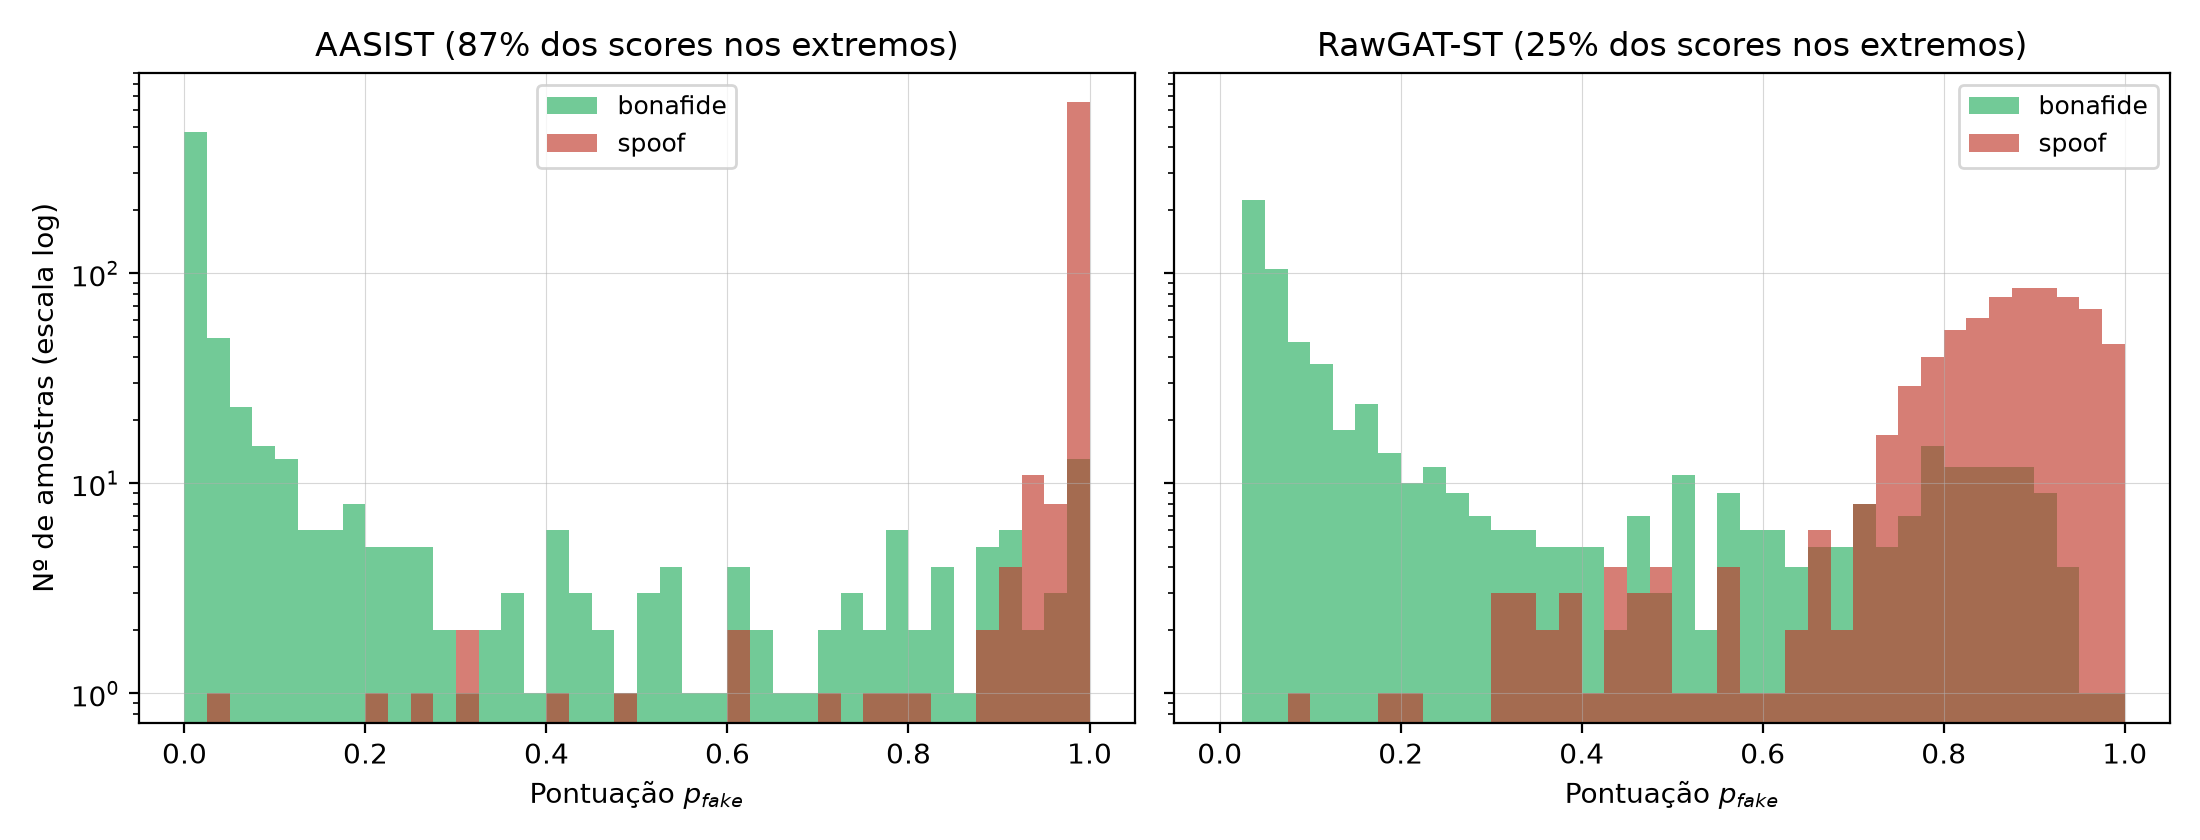
\includegraphics[width=0.95\textwidth]{figures/score_distributions_gat.png}
\caption[Distribuições da pontuação por classe para AASIST e RawGAT-ST]{%
Distribuições da pontuação $p_{\mathrm{fake}}$ por classe verdadeira
para AASIST e RawGAT-ST no conjunto de teste limpo, em escala logarítmica
(geradas por \texttt{scripts/reporting/export\_tcc\_extra\_figures.py}). A cabeça
AM-Softmax do AASIST concentra \num{86,5}\% dos \textit{scores} nos extremos
do intervalo, contra \num{24,5}\% no RawGAT-ST.}
\label{fig:score_distributions_gat}
\end{figure}

\begin{figure}[htbp]
\centering
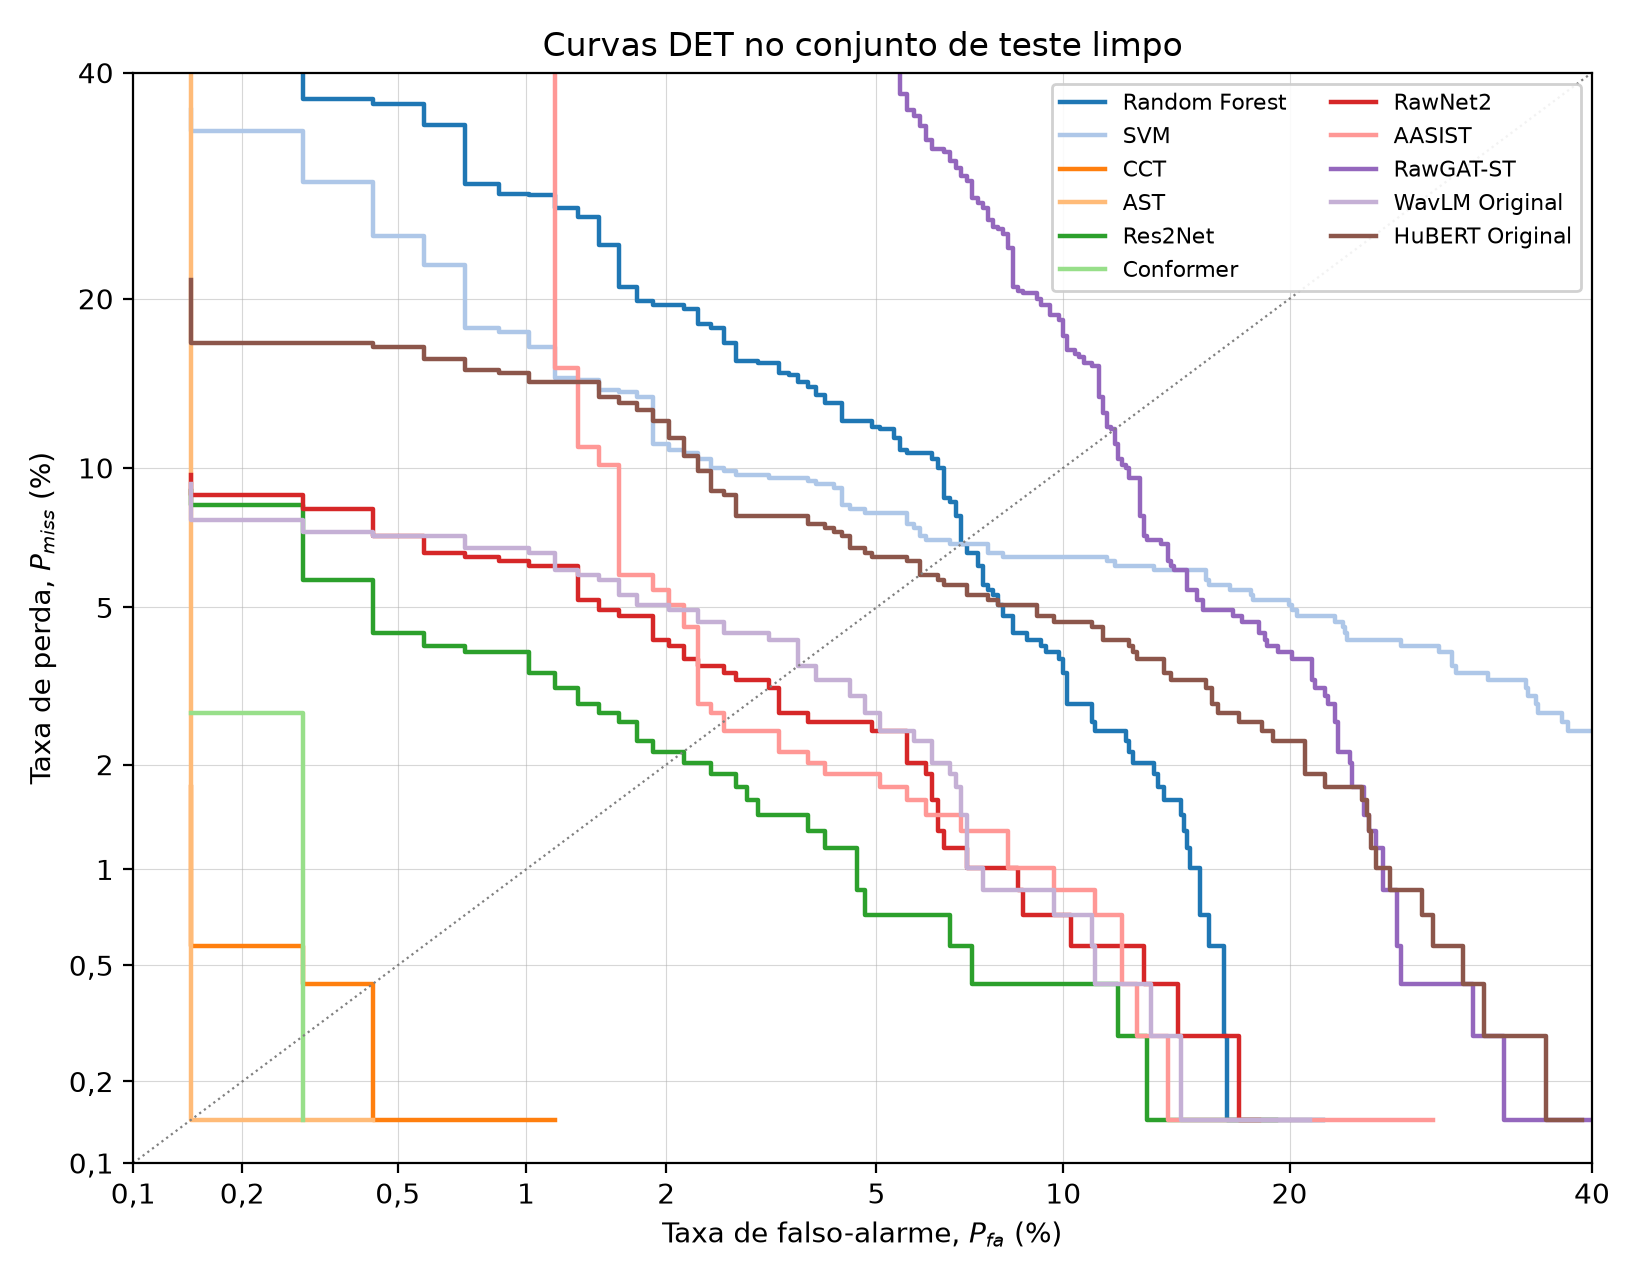
\includegraphics[width=0.9\textwidth]{figures/benchmark_det_curves.png}
\caption[Curvas DET dos onze modelos no conjunto de teste limpo]{%
Curvas DET (\textit{Detection Error Tradeoff}) dos \num{11} modelos
no conjunto de teste limpo, em eixos probit (geradas por
\texttt{scripts/reporting/export\_tcc\_extra\_figures.py}). A curva do AASIST
mostra a transição abrupta de $P_{\mathrm{miss}}$ na região de baixo $P_{\mathrm{fa}}$, efeito da
cauda de \textit{bonafide} com pontuação saturada no extremo incorreto.}
\label{fig:benchmark_det_curves}
\end{figure}

Segundo, o $t$-DCF$^\ast$ acompanha o ordenamento do EER, mas \emph{comprime}
as distâncias em vez de ampliá-las. Tomando o AST como referência, o RawGAT-ST
está \num{82} vezes acima em EER e apenas \num{76} vezes em $t$-DCF$^\ast$; a
compressão se repete em todos os dez pares, variando de \num{1}\% a
\num{35}\%. O efeito decorre da normalização por $\min(C_1, C_2)$
(Equação~\ref{eq:tdcf}): com os parâmetros do ASV fixados, o denominador impõe
uma escala comum que limita o quanto a razão entre dois detectores pode
crescer. A parametrização adotada (ASVspoof 2019 LA, com
$C_{\text{fa}} = 10 \gg C_{\text{miss}} = 1$) pondera fortemente a região de
baixa taxa de falso-alarme, mas esse peso atua sobre o \emph{formato} da curva
de erro de cada modelo, não sobre a distância entre modelos.

Cabe registrar, porém, um resultado negativo relevante: neste \textit{corpus} o
$t$-DCF$^\ast$ \textbf{não reordena o recorte}. Comparadas as posições nas duas
métricas, a única troca ocorre entre SVM e \textit{Random Forest}, que têm EER
numericamente idêntico (\num{6,95}\%) e são desempatados pelo custo. Os demais
nove modelos ocupam a mesma posição em ambas. A assimetria de custo
$C_{\text{fa}} = 10 \gg C_{\text{miss}} = 1$, portanto, não altera a escolha
\emph{entre} detectores aqui --- o que é informativo em si, e contraria a
expectativa de que uma métrica ponderada por custo produziria um ordenamento
distinto.

O que a ponderação revela não é uma troca de posições, e sim quanto cada modelo
é penalizado pela forma da sua curva de erro. A razão $t$-DCF$^\ast/$EER varia
de \num{1,86} (Conformer) a \num{2,86} (AST), e o AASIST fica entre os mais
penalizados (\num{2,77}) --- coerente com a sua cauda de falsos positivos e com
o salto de $P_{\mathrm{miss}}$ medido na curva DET. A leitura correta é, portanto, que a
assimetria de custo importa para escolher o \emph{ponto de operação} de um
detector já selecionado, e não para selecioná-lo. É também por isso que o
protocolo reporta as três métricas em conjunto: elas concordam no ordenamento,
mas descrevem regimes de operação diferentes.

\subsubsection{Vazamento de Domínio e Separabilidade}

Os valores de AUC-ROC muito próximos de \num{1,000} (CCT e Conformer,
\num{0,9999}) e os picos de acurácia de validação acima de \num{99}\%
(Conformer, \num{99,59}\% na época \num{69} ---
Tabela~\ref{tab:estabilidade_treinamento}) exigem interpretação cuidadosa.
Separabilidade quase perfeita é, em princípio, compatível tanto com um detector
genuinamente eficaz quanto com um classificador que explora correlações
espúrias entre fonte, canal e rótulo.

No caso deste protocolo, as três explicações espúrias mais comuns estão
descartadas por construção (Seção~\ref{sec:vazamento}): o pareamento mantém
texto e locutor constantes entre as classes, a disjunção dupla foi auditada com
sobreposição nula em quatro dimensões, e o oráculo majoritário fica no nível do
acaso para fonte, locutor e texto. Resta uma explicação legítima --- a de que
os clones XTTS-v2 carregam artefatos de \textit{vocoder} de fato detectáveis
--- e uma alternativa que este protocolo \emph{não} consegue afastar: a de que
os modelos aprenderam a assinatura \emph{daquele} sintetizador específico, e
não a distinguir fala natural de fala sintética em geral.

Essa segunda hipótese é a limitação real, e ela é de \textbf{generalização
entre geradores}, não de vazamento de partição. A separabilidade alta em um
\textit{corpus} de gerador único é o resultado esperado mesmo para um detector
que não generalizaria; distinguir os dois casos exige avaliação contra sistemas
de síntese não vistos no treino (Seção~\ref{sec:trabalhos_futuros}). Até lá, as
métricas devem ser lidas como desempenho contra o XTTS-v2, e não como
capacidade geral de detecção.

\subsubsection{Eficiência Computacional e Trade-offs}

A Tabela~\ref{tab:eficiencia_modelos} e as
Figuras~\ref{fig:benchmark_latency_size}
e~\ref{fig:benchmark_accuracy_latency_tradeoff} mostram que desempenho e custo
computacional não são monotonicamente relacionados (QP3). Uma ressalva
metodológica antecede a leitura: as latências da
Tabela~\ref{tab:eficiencia_modelos} foram medidas em três \textit{runtimes}
distintos (Seção~\ref{sec:ambiente_experimental}), de modo que os seus valores
absolutos \textbf{não formam um \textit{ranking} único}. Os
\SI{15,77}{\milli\second} do WavLM Original refletem PyTorch em GPU e não são
comparáveis aos \SI{50,46}{\milli\second} do Conformer em Keras, nem aos
\SI{0,90}{\milli\second} do SVM em scikit-learn sobre CPU.

\paragraph{Medição em dispositivo único.} Para remover essa confusão, os
\num{11} modelos foram remedidos em um \textbf{mesmo dispositivo} --- CPU, o
único denominador comum, já que SVM e \textit{Random Forest} não têm caminho de
GPU ---, sob protocolo idêntico ao original: lote unitário, duas execuções de
aquecimento, \num{30} medidas, mediana, e apenas a passagem direta do modelo,
sem \textit{front-end}. A Tabela~\ref{tab:latencia_cpu} traz o resultado, e ele
\textbf{reordena o recorte}.

\begin{table}[H]
\centering
\caption{Latência de inferência dos \num{11} modelos no \emph{mesmo}
dispositivo (CPU), contra os valores publicados em três \textit{runtimes}
distintos. A coluna \textit{Fator} é a razão entre as duas medidas.}
\label{tab:latencia_cpu}
\small\singlespacing
\begin{tabular}{@{}lrlrr@{}}
\toprule
\textbf{Modelo} & \textbf{Publicado} & \textbf{Ambiente} &
\textbf{CPU única} & \textbf{Fator} \\
\midrule
SVM                    & \num{0,90}  & CPU/sklearn  & \num{1,03}   & \num{1,1}$\times$ \\
Res2Net                & \num{46,41} & GPU/Keras    & \num{22,05}  & \num{0,5}$\times$ \\
CCT                    & \num{31,83} & GPU/Keras    & \num{24,05}  & \num{0,8}$\times$ \\
Conformer              & \num{50,46} & GPU/Keras    & \num{51,96}  & \num{1,0}$\times$ \\
\textit{Random Forest} & \num{56,43} & CPU/sklearn  & \num{64,70}  & \num{1,1}$\times$ \\
AASIST                 & \num{53,38} & GPU/Keras    & \num{94,82}  & \num{1,8}$\times$ \\
RawNet2                & \num{90,08} & GPU/Keras    & \num{119,26} & \num{1,3}$\times$ \\
RawGAT-ST              & \num{54,45} & GPU/Keras    & \num{176,81} & \num{3,2}$\times$ \\
AST                    & \num{44,46} & GPU/Keras    & \num{223,76} & \num{5,0}$\times$ \\
WavLM Original         & \num{15,77} & GPU/PyTorch  & \num{379,14} & \num{24,0}$\times$ \\
HuBERT Original        & \num{15,98} & GPU/PyTorch  & \num{395,35} & \num{24,7}$\times$ \\
\bottomrule
\end{tabular}

\vspace{2pt}
{\footnotesize Valores em milissegundos, mediana de \num{30} inferências de
amostra única.}
\end{table}

Três leituras seguem, e a primeira \textbf{corrige uma impressão que a tabela
original induzia}. Os dois \textit{backbones} SSL apareciam como os
\emph{mais rápidos} do recorte (\SI{15,77}{\milli\second} e
\SI{15,98}{\milli\second}); no mesmo dispositivo, são dos \emph{mais lentos},
com quase \num{400}~ms --- fator de \num{25}$\times$. A leitura anterior media a
GPU, não o modelo: \num{94,8}~milhões de parâmetros continuam sendo
\num{94,8}~milhões quando não há acelerador.

Segundo, dois modelos ficam \textbf{mais rápidos} em CPU do que os seus próprios
números de GPU --- Res2Net (\num{0,5}$\times$) e CCT (\num{0,9}$\times$). Não é
anomalia: em lote unitário, o custo de lançamento de núcleos na GPU domina o
tempo de redes pequenas, e a aceleração não se paga.

Terceiro, os modelos de áudio bruto ocupam a faixa intermediária-alta
(AASIST \SI{94,82}{\milli\second}, RawNet2 \SI{119,26}{\milli\second},
RawGAT-ST \SI{176,81}{\milli\second}), o que é coerente com o comprimento da
sequência que processam: \num{48000} amostras contra as \num{100} ou \num{300}
linhas dos mapas espectrais. O ordenamento por custo de inferência em
dispositivo comum é, portanto: SVM, Res2Net, CCT, Conformer, \textit{Random
Forest}, AASIST, RawNet2, RawGAT-ST, AST, WavLM e HuBERT.

\begin{infobox}{Condição de medição: por que os valores são de máquina ociosa}
Uma primeira série destas medidas foi tomada com a máquina sob carga (um
treinamento concorrente ocupava \num{8} dos \num{12} núcleos) e foi
\textbf{descartada}, porque a contenção distorceu os resultados de forma
\emph{muito} desigual. A maior parte dos modelos variou entre \num{0} e
\SI{14}{\percent} entre as duas séries, mas o \textbf{RawNet2 caiu
\SI{78,6}{\percent}} --- de \SI{556}{\milli\second} sob carga para
\SI{119,26}{\milli\second} em máquina ociosa --- deslocando-se da última para a
\num{7}.\textordfeminine\ posição.

O episódio é instrutivo. Sob a medida contaminada, o RawNet2 aparecia como o
modelo mais lento do recorte, e havia uma explicação mecanicista convincente à
mão: a sua GRU é sequencial por construção e não se beneficia de paralelismo.
A explicação era plausível, ajustava-se ao número --- e estava errada. Redes
recorrentes são sensíveis à disponibilidade de núcleos e ao escalonamento, o
que as torna as \emph{mais} penalizadas por contenção, não as mais lentas em
absoluto. Os valores da Tabela~\ref{tab:latencia_cpu} são os da máquina ociosa,
com o processo restrito aos mesmos \num{3} núcleos em ambas as séries para que
a única variável fosse a carga.
\end{infobox}

Feita a ressalva, o modelo mais compacto do conjunto é o \textbf{AASIST}
(\num{396312} parâmetros, \SI{1,88}{\megabyte}), que combina esse custo com a
\num{7}.\textordfeminine\ melhor acurácia limpa (\num{94,72}\%; \num{5}.\textordfeminine\
em EER) e a \num{2}.\textordfeminine\ melhor robustez a \SI{10}{\decibel} (\num{91,68}\%)
--- a relação custo-benefício mais favorável do recorte, com a ressalva do seu
$t$-DCF$^\ast$ discutida acima. O RawGAT-ST vem logo depois em tamanho
(\num{650204} parâmetros, \SI{2,80}{\megabyte}), mas com o pior desempenho do
conjunto em todas as métricas.

O SVM alia latência mínima (\SI{0,90}{\milli\second}) a acurácia de \num{93,20}\% em
condição limpa e \num{85,53}\% a \SI{10}{\decibel}, o que o torna atrativo sob
restrição severa de recursos --- desde que o ponto de operação não precise
sobreviver a SNR abaixo do visto em treino (Seção~\ref{sec:snr5}). O CCT ocupa
uma posição notável: com apenas \num{1,82}~milhão de parâmetros e
\SI{7,13}{\megabyte}, alcança \num{99,57}\% de acurácia limpa, a
\num{2}.\textordfeminine\ melhor do recorte --- duas ordens de grandeza mais
leve que o AST, com desempenho estatisticamente indistinguível dele.

No outro extremo, os \textit{backbones} SSL são os mais pesados
($\approx$\num{94,8}~milhões de parâmetros, $\approx$\SI{362}{\megabyte}), seguidos
pelo AST (\num{85,5}~milhões, \SI{326,73}{\megabyte}) e pelo Conformer
(\num{28,6}~milhões, \SI{110,23}{\megabyte}). Não há, portanto, um único modelo
dominante em todas as dimensões: a escolha depende de qual restrição ---
latência, memória, robustez ou custo de falso-alarme --- é prioritária na
aplicação-alvo.

\subsubsection{Estabilidade de Treinamento}

A Tabela~\ref{tab:estabilidade_treinamento} e a
Figura~\ref{fig:training_stability} mostram sete dos nove modelos neurais
convergindo de forma estável. Os picos de validação ocorrem em épocas variadas
--- HuBERT Original na \num{12}, Res2Net e RawGAT-ST na \num{17}, RawNet2 na
\num{30}, AST na \num{33}, CCT na \num{48}, AASIST na \num{52}, WavLM Original
na \num{57} e Conformer na \num{69} ---, sem convergência precoce sistemática
sob o protocolo com \textit{augmentation} de ruído no treino.

Duas observações sobre a leitura dessa tabela. A coluna \textit{Época} registra
o pico da \emph{acurácia} de validação, grandeza descritiva da curva; o
\textit{checkpoint} avaliado é o de menor \emph{perda} de validação limpa
(Seção~\ref{sec:protocolo_treinamento}), e os dois critérios podem apontar
épocas distintas. E a coluna \textit{Queda} é a diferença pico$-$final, que a
própria legenda adverte não demonstrar estabilidade: os indicadores do
diagnóstico automático são outros e vêm do campo \path{training_stability}
de cada \path{results.json}, citados a seguir.

\textbf{Dois modelos violam o critério de estabilidade} adotado (desvio do
monitor $\leq 0{,}02$ nas últimas \num{50} épocas e queda máxima entre épocas
consecutivas $\leq 0{,}20$), e ambos são classificados automaticamente como
\path{unstable_oscillation} pelo diagnóstico do \textit{pipeline}:

\begin{itemize}
    \item \textbf{Conformer} --- desvio de \num{0,0963} na cauda (quase cinco
    vezes o critério) e queda máxima de \num{0,4890} entre épocas consecutivas,
    a maior do recorte. É o caso mais grave, e recai justamente sobre o
    \num{3}.\textordmasculine\ melhor modelo do trabalho. Note-se que a coluna
    \textit{Queda} da Tabela~\ref{tab:estabilidade_treinamento} registra
    \num{0,34}\% para o Conformer, a \emph{menor} do recorte: é a diferença
    pico$-$final, que nada diz sobre a oscilação percorrida entre as duas
    pontas. As duas grandezas medem coisas diferentes e não se contradizem.
    \item \textbf{RawGAT-ST} --- desvio de \num{0,0274} e queda máxima de
    \num{0,2232}, com o melhor \textit{checkpoint} ocorrendo já na época
    \num{17} de \num{100} e degradação sustentada depois disso
    ($val\_loss$ de \num{0,511} no melhor ponto contra \num{1,18} ao final):
    a assinatura clássica de sobreajuste.
\end{itemize}

A consequência metodológica é relevante e precisa ser declarada: sob oscilação
dessa magnitude, a época selecionada pelo critério de menor $val\_loss$ limpa
depende parcialmente do \emph{ruído} da curva de validação, e não apenas do
mérito do modelo naquele ponto. Uma reexecução com outra semente poderia
selecionar uma época distinta e produzir métricas apreciavelmente diferentes
para esses dois modelos --- ao contrário dos outros sete, cujas curvas são
planas na cauda. Os resultados do Conformer e do RawGAT-ST devem, portanto, ser
lidos com uma margem de incerteza maior que a dos demais, e o RawGAT-ST em
particular é candidato natural a retreinamento com regularização reforçada.

\subsubsection{Ressalva sobre Execução Única}

Todos os resultados reportados correspondem a uma única execução por modelo, sem
repetição sobre múltiplas sementes aleatórias de inicialização e
particionamento. Diferenças pequenas entre modelos próximos, como AST e
CCT (\num{99,71}\% vs.\ \num{99,57}\% de acurácia), não devem ser
interpretadas como estatisticamente significativas. Uma régua útil é o
intervalo de confiança de Wilson a \num{95}\% para a acurácia, que quantifica
apenas a incerteza amostral do conjunto de teste
($n = \num[group-minimum-digits=4]{1382}$): no topo, \num{99,71}\% corresponde a
$[\num{99,26}\%;\, \num{99,89}\%]$; no modelo de menor acurácia,
\num{87,55}\% corresponde a $[\num{85,71}\%;\, \num{89,19}\%]$. O intervalo de
Wilson \textbf{não é simétrico} em torno da proporção observada --- e quanto
mais próxima de $1$ ela está, mais assimétrico ele fica ---, razão pela qual se
reporta o intervalo, e não uma margem $\pm$.
Sob essa régua --- e sob os testes pareados por \textit{cluster} com correção
de Holm, que não rejeitam a hipótese nula para nenhum par entre AST, CCT e
Conformer ---, o topo do recorte é indistinguível, enquanto as diferenças de
robustez a \SI{10}{\decibel}
discutidas acima --- de \num{15,2} pontos percentuais entre os extremos
(Res2Net, \num{92,40}\%; RawGAT-ST, \num{77,21}\%) ---
excedem em muito a incerteza amostral. Note-se que esse intervalo não captura
a variância de treinamento (inicialização, ordem dos lotes), que só múltiplas
execuções revelariam. A magnitude dos efeitos discutidos acima
(robustez a ruído e diferença entre famílias de modelos) é suficiente para uma
interpretação qualitativa, mas comparações finas entre os modelos de melhor
colocação exigiriam múltiplas execuções com relato de média e desvio-padrão.

A leitura das métricas deve ser feita, portanto, com parcimônia: os resultados
caracterizam desempenho em distribuição fechada e dependem do \textit{corpus},
das fontes de geração e do protocolo de particionamento utilizado. A eficiência
computacional, a estabilidade e, sobretudo, a robustez a ruído são parte
essencial da interpretação, não apenas complementos gráficos ao desempenho no
conjunto limpo.

\newpage

% =====================================================================
%  7. CONCLUSÕES
% =====================================================================
\section{Conclusões}
\label{sec:conclusao}

Este trabalho desenvolveu e avaliou um \textit{pipeline} modular e de código
aberto para detecção de áudio sintético em português, submetendo \num{11}
modelos heterogêneos --- de classificadores estatísticos clássicos a redes
espectro-temporais e \textit{backbones} auto-supervisionados --- a um protocolo
comum de treinamento, inferência e \textit{benchmark}. Nesse sentido, os
objetivos específicos e as questões de pesquisa delineados na
Seção~\ref{sec:introducao} foram atendidos:
consolidou-se uma base balanceada com particionamento reprodutível,
implementou-se o pré-processamento acústico e a extração de características, e
os modelos foram comparados sob métricas de acurácia, F1-\textit{score},
AUC-ROC, EER, $t$-DCF, latência, tamanho de artefato e robustez a ruído.

\subsection*{Resposta às Questões de Pesquisa}

\textbf{QP1 --- como as famílias se comparam sob protocolo único.} No conjunto
de teste limpo lideram as arquiteturas espectro-temporais densas, com AST, CCT
e Conformer acima de \num{98}\% de acurácia; os testes pareados, porém, não
separam os três, que constituem \textbf{empate técnico}
(Seção~\ref{sec:analise_resultados}). A primeira colocação do AST não isola
mérito arquitetural: ele é o único modelo do recorte que parte de pesos
pré-treinados e o único que recebe a grade espectral mais fina
(Seção~\ref{sec:caracteristicas}). A ablação executada
(Seção~\ref{sec:ablacao_ast}) quantifica a primeira dessas vantagens e
\textbf{reverte o ordenamento}: sem os pesos AudioSet, o AST cai a
\num{94,93}\%, abaixo de CCT, Conformer e Res2Net --- todos treinados do zero.
A topologia ViT-Base não é, portanto, superior às alternativas neste
\textit{corpus}; o que a colocava em primeiro lugar era o pré-treinamento em
larga escala, que vale \num{4,78} pontos percentuais de acurácia e multiplica o
EER por \num{30}. Os \textit{backbones} auto-supervisionados
congelados ficaram na metade inferior --- posição que contrasta com a literatura
recente, em que \textit{front-ends} SSL figuram entre os melhores sistemas. A
explicação mais provável está no \textit{back-end} raso aqui empregado (um
perceptron sobre \textit{pooling} global), e não no congelamento em si; o
ajuste fino integral permanece como caminho não explorado, ao custo de duas
ordens de grandeza a mais de parâmetros treináveis.

\textbf{QP2 --- se a acurácia limpa prediz a robustez.} Não prediz, e esse é o
achado central. Sob ruído o ordenamento se reorganiza: AST e CCT deixam o bloco
de topo, e o RawGAT-ST separa-se de todos os demais como o menos robusto. O que
os dados sustentam é o deslocamento \emph{entre blocos}, não a ordem dentro
deles --- a \SI{10}{\decibel} os cinco primeiros formam um conjunto mutuamente
indistinguível por McNemar e por \textit{bootstrap} de EER.

Quanto aos \emph{fatores} que explicam a dissociação, a resposta é
\textbf{negativa em três frentes}. A representação de entrada não explica:
AASIST e RawGAT-ST partilham forma de onda e \textit{front-end} SincConv e
separam-se por \num{14,5} pontos percentuais. A capacidade tampouco: são os dois
menores modelos do recorte. E o diagnóstico automático de estabilidade também
não ordena --- o Conformer recebe o mesmo rótulo de instabilidade do RawGAT-ST e
é o \num{3}.\textordmasculine\ mais robusto do conjunto. O sobreajuste do
RawGAT-ST permanece a leitura mais econômica para aquele par específico, mas com
$n = 2$ é hipótese para trabalho futuro, não achado estabelecido. O fator
discriminante da robustez a ruído \textbf{não foi identificado}, e delimitá-lo
exigiria as múltiplas sementes que este recorte não tem.

No nível \emph{não visto} de \SI{5}{\decibel} (Seção~\ref{sec:snr5}), o SVM
revela falha de natureza distinta: colapsa a \num{58,68}\% de acurácia mantendo
AUC-ROC de \num{0,884} --- perda de calibração, não de capacidade
discriminativa. A ressalva importa: essa perda \emph{não} é recuperável pelos
meios disponíveis, já que o limiar calibrado fora do teste piora o resultado e o
teto de \num{79,59}\% exige um oráculo ajustado na própria partição de
avaliação.

\textbf{QP3 --- compromissos de custo e modelo dominante.} Nenhum modelo domina
simultaneamente acurácia, robustez, latência e memória. Três perfis se destacam
por razões distintas: o \textbf{CCT}, com desempenho indistinguível do AST a
duas ordens de grandeza menos parâmetros; o \textbf{Res2Net}, que encabeça a
robustez a \SI{10}{\decibel} a custo intermediário; e o \textbf{SVM}, de
latência mínima em CPU, com duas ressalvas que pesam sobre a recomendação --- o
ponto de operação não sobrevive a SNR abaixo do visto em treino e a acurácia
despenca a \num{54,03}\% no pior dos \num{11} locutores de teste. Os
\textit{backbones} SSL, os mais pesados do conjunto, não compensam o custo neste
protocolo.

A remedição em dispositivo único (Tabela~\ref{tab:latencia_cpu}) reforça esse
último ponto e desfaz uma impressão da tabela original: WavLM e HuBERT
\emph{pareciam} os modelos mais rápidos do recorte
($\approx\SI{16}{\milli\second}$), mas aquilo media a GPU, não o modelo. Em
dispositivo comum eles gastam quase \SI{400}{\milli\second} --- fator de
\num{24}$\times$ --- e passam a ser os \textbf{dois mais lentos} do recorte.
Res2Net e CCT, ao contrário,
são \emph{mais rápidos} em CPU do que os seus próprios números de GPU, porque em
lote unitário o custo de lançamento na GPU domina o tempo de redes pequenas.
Para implantação sem acelerador --- o cenário mais comum em produção --- o
compromisso favorece SVM, Res2Net e CCT, e desaconselha os SSL.

O custo de \emph{treinamento} acrescenta uma quarta dimensão que não acompanha
as demais: RawGAT-ST e AASIST consomem \num{67}\% das \SI{63,3}{\hour} do
\textit{benchmark} e terminam nas duas piores posições entre os neurais, enquanto
o CCT alcança o segundo melhor resultado em menos de uma hora. O que domina é o
custo por passo da topologia, não a contagem de parâmetros --- os grafos de
atenção dinâmicos do RawGAT-ST, com \num{650} mil parâmetros, treinam em mais
que o dobro do tempo do AST, com \num{85,5}~milhões. É a dimensão de custo que
mais pesa para quem itera sobre o detector, e a que menos aparece nas
comparações usuais da literatura.

\subsection*{Duas Ressalvas de Validade}

A \textbf{dispersão entre locutores não vistos} qualifica todas as médias
reportadas (Seção~\ref{sec:pior_locutor}). O SVM cai de \num{93,20}\% de média
para \num{54,03}\% no pior dos \num{11} falantes do teste --- quatro pontos
acima do acaso ---, e RawGAT-ST, HuBERT Original, \textit{Random Forest} e
RawNet2 exibem o mesmo padrão em grau menor. Só AST e CCT mantêm, no pior
locutor, desempenho próximo da própria média. Em biometria de voz essa
concentração do erro significa exclusão sistemática de indivíduos, e não
degradação difusa: é um risco que nenhuma métrica agregada capta.

A \textbf{separabilidade elevada} exige leitura cuidadosa. Os valores de AUC-ROC
próximos da unidade não decorrem de vazamento de partição --- o protocolo audita
sobreposição nula em locutor, frase, texto e conteúdo, e o oráculo majoritário
fica no nível do acaso (Seção~\ref{sec:vazamento}). São compatíveis, porém, com
a hipótese de que os modelos aprenderam a assinatura do \emph{gerador
específico} usado (XTTS-v2), e não a distinguir fala natural de fala sintética
em geral. As métricas reportadas devem, portanto, ser entendidas como desempenho
contra aquele sintetizador, não como estimativa de generalização para geradores
não vistos ou condições reais de canal.

\subsection{Principais Contribuições}

\begin{itemize}
    \item Um \textit{pipeline} reprodutível e de código aberto que padroniza
    pré-processamento, treinamento, inferência e geração automática de
    relatórios de \textit{benchmark} para detecção de áudio sintético em
    português.
    \item Uma comparação empírica de \num{11} arquiteturas heterogêneas sob
    protocolo único, contemplando eficiência computacional e robustez a ruído
    AWGN, em \textit{corpus} de fala em português brasileiro.
    \item Um \textbf{protocolo de avaliação auditável} para detecção de áudio
    sintético em português: \textit{corpus} pareado (mesma locução, mesmo
    locutor, clonada), partição por disjunção dupla locutor $\times$ frase com
    sobreposição verificada em quatro dimensões, congelamento criptográfico da
    partição de teste anterior ao treinamento confirmatório e oráculo
    majoritário reportado como evidência de ausência de atalho. Cada artefato
    de resultado carrega essas verificações, de modo que a alegação de
    integridade do protocolo é conferível, e não declarativa.
    \item Uma comparação estatística pareada entre todos os pares de modelos
    (McNemar e \textit{bootstrap} agrupados por frase, com correção de Holm
    sobre \num{55} comparações), que distingue diferenças reais de ruído
    amostral --- e mostra que o topo do recorte é um empate técnico.
    \item Uma \textbf{implementação de referência operável}
    (Apêndice~\ref{sec:sistema}), em que os \num{11} modelos avaliados são servidos
    por três interfaces sobre o mesmo núcleo de domínio --- API REST, interface
    interativa e CLI ---, empacotada em contêineres e restrita aos artefatos
    promovidos. Ela fecha o percurso da QP3: a escolha do detector deixa de ser
    uma linha de tabela e passa a ser uma configuração de implantação.
\end{itemize}

\subsection{Limitações}
\label{sec:limitacoes}

As conclusões restringem-se ao \textit{corpus} e ao gerador avaliados. As
principais limitações são:

\begin{enumerate}[label=(\roman*)]
    \item \textbf{Gerador único.} Toda a classe sintética provém do XTTS-v2.
    Os resultados medem a detecção \emph{daquele} processo de síntese; a
    generalização para geradores não vistos --- regime avaliado por campanhas
    como o ASVspoof, com dezenas de ataques --- permanece não medida, e é a
    limitação mais relevante para validade externa.
    \item \textbf{Fonte única e canal homogêneo.} O \textit{corpus} deriva de
    uma única base (CETUC), com condições de gravação uniformes. A robustez a
    degradações reais de canal (codecs, reverberação, ruído não estacionário)
    não é avaliada: o AWGN cobre apenas degradação aditiva estacionária.
    \item \textbf{Execução única por modelo}, sem repetição sobre múltiplas
    sementes, o que impede estimar variância de treinamento. A limitação pesa
    especialmente sobre Conformer e RawGAT-ST, cujas curvas de validação
    oscilam o bastante para que a época selecionada dependa parcialmente de
    ruído (Seção~\ref{sec:analise_resultados}).
    \item \textbf{SSL apenas com \textit{backbone} congelado}, sem ajuste fino
    integral --- condição que a literatura recente indica ser determinante para
    o desempenho dessa família.
    \item \textbf{$t$-DCF como \textit{proxy} interno}, sem acoplamento a um
    sistema ASV oficial; os valores são comparáveis entre si, mas não com os
    publicados em campanhas ASVspoof.
    \item \textbf{Latências da Tabela~\ref{tab:eficiencia_modelos} não
    comparáveis entre \textit{runtimes}}: medidas em TensorFlow/GPU,
    PyTorch/GPU e scikit-learn/CPU, valem como ordem de grandeza dentro de cada
    ambiente. A limitação foi \textbf{sanada} por uma remedição em dispositivo
    único e máquina ociosa (Tabela~\ref{tab:latencia_cpu}), que estabelece o
    ordenamento comparável entre as onze arquiteturas.
    \item \textbf{Artefato do RawGAT-ST anterior ao ajuste de regularização.}
    O modelo publicado foi treinado antes do último ajuste de
    \textit{dropout}, regularização $L_2$ e cronograma de decaimento; seus
    números tendem a melhorar em um retreinamento, e devem ser lidos como
    limite inferior para essa arquitetura.
    \item \textbf{Os classificadores clássicos não são cegos ao conjunto de
    teste.} O vetor tabular passou de \num{63} para \num{183} descritores
    depois de uma rodada exploratória em que SVM e \textit{Random Forest}
    perderam o ponto de operação a \SI{5}{\decibel}
    (Seção~\ref{sec:caracteristicas}). O congelamento criptográfico da partição
    protege os nove modelos neurais, cuja configuração não foi tocada após o
    selo, mas não esses dois: o seu \textit{front-end} de entrada foi escolhido
    com conhecimento de um resultado de teste, e as suas métricas são
    estimativa otimista. O custo dessa não cegueira foi \textbf{medido} sobre
    uma partição fresca de \num{4916} amostras
    (Seção~\ref{sec:avaliacao_cega}): \num{2,6} e \num{3,5} pontos percentuais
    de acurácia para SVM e \textit{Random Forest}, com degradação maior nas
    métricas de ordenação. A limitação, portanto, é conhecida em magnitude ---
    e não invalida as conclusões sobre os clássicos, apenas as desloca.
    \item \textbf{Front-end espectral não uniforme.} O AST opera sobre mapas
    $300 \times 128$ e parte de pesos AudioSet, enquanto Conformer, CCT e
    Res2Net operam sobre $100 \times 80$ e treinam do zero
    (Seção~\ref{sec:caracteristicas}). Das duas variáveis confundidas, o
    \textbf{pré-treinamento foi isolado e medido}
    (Seção~\ref{sec:ablacao_ast}): vale \num{4,78} pontos de acurácia, e a sua
    remoção derruba o AST abaixo das três redes treinadas do zero. Permanece
    não atribuída a parcela devida à \emph{resolução}, que exigiria um segundo
    braço ($100 \times 80$ com pesos transferidos).
\end{enumerate}

\subsection{Trabalhos Futuros}
\label{sec:trabalhos_futuros}

A prioridade, decorrente das limitações (i) e (ii), é a avaliação
\textbf{\textit{cross-generator}}: incluir na partição de teste amostras de
sintetizadores ausentes do treino --- outros modelos zero-shot, sistemas de
conversão de voz e \textit{vocoders} de arquitetura distinta --- para separar a
detecção de artefatos gerais de síntese do reconhecimento da assinatura do
XTTS-v2. É esse ensaio que converte as métricas aqui reportadas em estimativa
de capacidade de detecção, e não apenas de desempenho contra um gerador.

Em segundo lugar, a validação \textbf{\textit{cross-dataset}}, com bases de
proveniência e condições de gravação distintas, mede a sensibilidade a canal
que o \textit{corpus} homogêneo atual não expõe --- complementada por ensaios
de robustez contra compressão por codec, reverberação e ruído real, mais
representativos do que o AWGN.

No protocolo de avaliação, três extensões diretas: (a) repetir o
\textit{benchmark} sobre múltiplas sementes com relato de média e
desvio-padrão, quantificando a variância de treinamento que o intervalo de
confiança amostral não captura --- prioritário para Conformer e RawGAT-ST, os
dois modelos com oscilação de validação; (b) retreinar o RawGAT-ST com a
regularização ajustada (limitação (vii)) e reavaliar sua posição no recorte; e
(c) re-medir a latência de todos os modelos em um único \textit{runtime} e
dispositivo de referência, tornando a dimensão de custo comparável entre
famílias.

Da limitação (ix) resta \emph{um} braço de ablação. O primeiro --- grade
$300 \times 128$ com \texttt{pretrained = false} --- já foi executado e é
relatado na Seção~\ref{sec:ablacao_ast}: isola o pré-treinamento e mostra que
ele responde por \num{4,78} pontos percentuais de acurácia, além de reverter a
posição do AST no recorte. Falta o braço complementar, grade $100 \times 80$
com \texttt{pretrained = true}, que isolaria a contribuição da \emph{resolução}
mantendo os pesos transferidos. Com ele, somado à configuração publicada e ao
braço já executado, o fatorial $2 \times 2$ se fecha e a parcela devida a cada
fator torna-se integralmente atribuível.

A limitação (viii) já foi quantificada na Seção~\ref{sec:avaliacao_cega}; o
passo remanescente é estender esse mesmo desenho de partição fresca aos nove
modelos neurais, de modo que todo o recorte --- e não apenas os clássicos ---
disponha de uma estimativa fora da amostra que orientou qualquer decisão.

Por fim, destacam-se a pertinência de adotar o $t$-DCF padronizado acoplado a
um sistema ASV de referência, avaliar os \textit{backbones} SSL com ajuste fino
integral e com \textit{back-ends} mais expressivos que o perceptron sobre
\textit{pooling} global, e incorporar métricas de calibração e explicabilidade
local (SHAP, Grad-CAM) ao relatório automático do \textit{pipeline}.



\newpage


% =====================================================================
%  REFERÊNCIAS
% =====================================================================
\begin{thebibliography}{99}

\bibitem{jia2018}
JIA, Y. et al.
Transfer learning from speaker verification to multispeaker text-to-speech
synthesis.
In: \textbf{Advances in Neural Information Processing Systems (NeurIPS)},
v.~31, 2018.

\bibitem{dudley1939}
DUDLEY, H.
The vocoder.
\textbf{Bell Labs Record},
v.~18, n.~4, p.~122--126, 1939.

\bibitem{klatt1987}
KLATT, D.~H.
Review of text-to-speech conversion for English.
\textbf{The Journal of the Acoustical Society of America},
v.~82, n.~3, p.~737--793, 1987.

\bibitem{hunt1996}
HUNT, A.~J.; BLACK, A.~W.
Unit selection in a concatenative speech synthesis system using a large
speech database.
In: \textbf{IEEE International Conference on Acoustics, Speech, and Signal
Processing (ICASSP)}, 1996.

\bibitem{oord2016wavenet}
VAN DEN OORD, A. et al.
WaveNet: A generative model for raw audio.
\textbf{arXiv preprint} arXiv:1609.03499, 2016.

\bibitem{wang2017}
WANG, Y. et al.
Tacotron: Towards end-to-end speech synthesis.
In: \textbf{Proc.\ Interspeech 2017}, 2017.

\bibitem{wang2023vall}
WANG, C. et al.
VALL-E: Neural Codec Language Models are Zero-Shot Text-to-Speech Synthesizers.
\textbf{arXiv preprint} arXiv:2301.02111, 2023.
Disponível em: \url{https://arxiv.org/abs/2301.02111}.
Acesso em: 15 jun.\ 2025.

\bibitem{mai2023warning}
MAI, K.~T. et al.
Warning: humans cannot reliably detect speech deepfakes.
\textbf{PLOS ONE},
v.~18, n.~8, e0285333, 2023.

\bibitem{heidari2024deepfake}
HEIDARI, A. et al.
Deepfake detection using deep learning methods: A systematic and comprehensive
review.
\textbf{WIREs Data Mining and Knowledge Discovery},
v.~14, n.~2, e1520, 2024.

\bibitem{shen2018natural}
SHEN, J. et al.
Natural TTS Synthesis by Conditioning WaveNet on Mel Spectrogram Predictions.
In: \textbf{IEEE International Conference on Acoustics, Speech and Signal
Processing (ICASSP)}, p.~4779--4783, 2018.

\bibitem{bird2023realtime}
BIRD, J. J.; LOTFI, A.
Real-time Detection of AI-Generated Speech for DeepFake Voice Conversion.
\textbf{arXiv preprint} arXiv:2308.12734, 2023.
Disponível em: \url{https://arxiv.org/abs/2308.12734}.
Acesso em: 15 jun.\ 2025.

\bibitem{pindrop2025}
PINDROP.
\textbf{Deepfake Trends to Look Out for in 2025}.
2025.
Disponível em: \url{https://www.pindrop.com/article/deepfake-trends/}.
Acesso em: 15 jun.\ 2025.

\bibitem{dfrlab2024}
FARRUGIA, B.
Brazil's electoral deepfake law tested as AI-generated content targeted local
elections.
\textbf{Digital Forensic Research Lab (Atlantic Council)}, 26 nov.\ 2024.
Disponível em:
\url{https://dfrlab.org/2024/11/26/brazil-election-ai-deepfakes/}.
Acesso em: 15 jun.\ 2025.

\bibitem{farrugia2024}
FARRUGIA, B.
The challenges of identifying deepfakes ahead of the 2024 Brazil election.
\textbf{Digital Forensic Research Lab (Atlantic Council)}, 2 out.\ 2024.
Disponível em: \url{https://dfrlab.org/2024/10/02/brazil-election-ai-research/}.
Acesso em: 15 jun.\ 2025.

\bibitem{todisco2019asvspoof}
TODISCO, M. et al.
ASVspoof 2019: Future Horizons in Spoofed and Fake Speech Detection.
In: \textbf{Proc.\ Interspeech 2019}, p.~1008--1012, 2019.

\bibitem{yamagishi2021asvspoof}
YAMAGISHI, J. et al.
ASVspoof 2021: Accelerating Progress in Spoofed and Deepfake Speech Detection.
In: \textbf{Proc.\ ASVspoof 2021 Workshop}, p.~47--54, 2021.

\bibitem{wang2024asvspoof5}
WANG, X. et al.
ASVspoof 5: Crowdsourced Speech Data, Deepfakes, and Adversarial Attacks at
Scale.
\textbf{arXiv preprint} arXiv:2408.08739, 2024.
Disponível em: \url{https://arxiv.org/abs/2408.08739}.
Acesso em: 15 jun.\ 2025.

\bibitem{yi2022add}
YI, J. et al.
ADD 2022: The First Audio Deep Synthesis Detection Challenge.
In: \textbf{IEEE International Conference on Acoustics, Speech and Signal
Processing (ICASSP)}, p.~9216--9220, 2022.

\bibitem{ren2019fastspeech}
REN, Y. et al.
FastSpeech: Fast, Robust and Controllable Text to Speech.
In: \textbf{Advances in Neural Information Processing Systems (NeurIPS)},
v.~32, 2019.

\bibitem{kim2021conditional}
KIM, J.; KONG, J.; SON, J.
Conditional Variational Autoencoder with Adversarial Learning for End-to-End
Text-to-Speech.
In: \textbf{International Conference on Machine Learning (ICML)},
p.~5530--5540, 2021.

\bibitem{casanova2022yourtts}
CASANOVA, E. et al.
YourTTS: Towards Zero-Shot Multi-Speaker TTS and Zero-Shot Voice Conversion
for everyone.
In: \textbf{International Conference on Machine Learning (ICML)},
p.~2709--2720, 2022.

\bibitem{fakevoices_card}
UNFAKE.
Fake Voices dataset card.
\textbf{Hugging Face Datasets}, 2026.
Disponível em: \url{https://huggingface.co/datasets/unfake/fake_voices}.
Acesso em: 27 jun.\ 2026.

\bibitem{kameoka2018stargan}
KAMEOKA, H. et al.
StarGAN-VC: Non-parallel many-to-many voice conversion using star generative
adversarial networks.
In: \textbf{IEEE Spoken Language Technology Workshop (SLT)},
p.~266--273, 2018.

\bibitem{cortes1995support}
CORTES, C.; VAPNIK, V.
Support-vector networks.
\textbf{Machine Learning},
v.~20, p.~273--297, 1995.

\bibitem{hochreiter1997lstm}
HOCHREITER, S.; SCHMIDHUBER, J.
Long Short-Term Memory.
\textbf{Neural Computation},
v.~9, n.~8, p.~1735--1780, 1997.

\bibitem{wu2015asvspoof}
WU, Z. et al.
ASVspoof 2015: the First Automatic Speaker Verification Spoofing and
Countermeasures Challenge.
In: \textbf{Proc.\ Interspeech 2015}, p.~2037--2041, 2015.

\bibitem{sahidullah2015comparison}
SAHIDULLAH, M. et al.
A Comparison of Features for Synthetic Speech Detection.
In: \textbf{Proc.\ Interspeech 2015}, p.~2087--2091, 2015.

\bibitem{todisco2016new}
TODISCO, M.; DELGADO, H.; EVANS, N.
A New Feature for Automatic Speaker Verification Anti-Spoofing:
Constant Q Cepstral Coefficients.
In: \textbf{Proc.\ Odyssey 2016 --- The Speaker and Language Recognition
Workshop}, p.~283--290, 2016.

\bibitem{lavrentyeva2017audio}
LAVRENTYEVA, G. et al.
Audio Replay Attack Detection with Deep Learning Frameworks.
In: \textbf{Proc.\ Interspeech 2017}, p.~82--86, 2017.

\bibitem{gao2021res2net}
GAO, S. et al.
Res2Net: A New Multi-Scale Backbone Architecture.
\textbf{IEEE Transactions on Pattern Analysis and Machine Intelligence},
v.~43, n.~2, p.~652--662, 2021.

\bibitem{tak2021rawnet2}
TAK, H. et al.
End-to-End Anti-Spoofing with RawNet2.
In: \textbf{IEEE International Conference on Acoustics, Speech and Signal
Processing (ICASSP)}, p.~6369--6373, 2021.

\bibitem{jung2022aasist}
JUNG, J.~W. et al.
AASIST: Audio Anti-Spoofing using Integrated Spectro-Temporal Graph Attention
Networks.
In: \textbf{IEEE International Conference on Acoustics, Speech and Signal
Processing (ICASSP)}, p.~6367--6371, 2022.

\bibitem{chen2022wavlm}
CHEN, S. et al.
WavLM: Large-Scale Self-Supervised Pre-Training for Full Stack Speech
Processing.
\textbf{IEEE Journal of Selected Topics in Signal Processing},
v.~16, n.~6, p.~1505--1518, 2022.

\bibitem{hsu2021hubert}
HSU, W.-N. et al.
HuBERT: Self-Supervised Speech Representation Learning by Masked Prediction
of Hidden Units.
\textbf{IEEE/ACM Transactions on Audio, Speech, and Language Processing},
v.~29, p.~3451--3460, 2021.

\bibitem{baevski2020wav2vec}
BAEVSKI, A. et al.
wav2vec 2.0: A Framework for Self-Supervised Learning of Speech
Representations.
\textbf{Advances in Neural Information Processing Systems (NeurIPS)},
v.~33, p.~12449--12460, 2020.

\bibitem{gong2021ast}
GONG, Y.; CHUNG, Y.; GLASS, J.
AST: Audio Spectrogram Transformer.
In: \textbf{Proc.\ Interspeech 2021}, p.~571--575, 2021.

\bibitem{vaswani2017attention}
VASWANI, A. et al.
Attention Is All You Need.
In: \textbf{Advances in Neural Information Processing Systems (NeurIPS)},
v.~30, 2017.

\bibitem{dosovitskiy2021vit}
DOSOVITSKIY, A. et al.
An Image is Worth 16x16 Words: Transformers for Image Recognition at Scale.
In: \textbf{International Conference on Learning Representations (ICLR)}, 2021.

\bibitem{brspeechdf_card}
AKCIT-DEEPFAKE.
BRSpeech-DF dataset card.
\textbf{Hugging Face Datasets}, 2026.
Disponível em: \url{https://huggingface.co/datasets/AKCIT-Deepfake/BRSpeech-DF}.
Acesso em: 27 jun.\ 2026.

\bibitem{muller2022does}
MÜLLER, N.~M. et al.
Does Audio Deepfake Detection Generalize?
In: \textbf{Proc.\ Interspeech 2022}, p.~2783--2787, 2022.

\bibitem{tak2021rawgatst}
TAK, H. et al.
End-to-End Spectro-Temporal Graph Attention Networks for Speaker Verification
Anti-Spoofing and Speech Deepfake Detection.
In: \textbf{Proc.\ ASVspoof 2021 Workshop}, p.~1--8, 2021.

\bibitem{gulati2020conformer}
GULATI, A. et al.
Conformer: Convolution-augmented Transformer for Speech Recognition.
In: \textbf{Proc.\ Interspeech 2020}, p.~5036--5040, 2020.

\bibitem{hassani2021cct}
HASSANI, A. et al.
Escaping the Big Data Paradigm with Compact Transformers.
\textbf{arXiv preprint} arXiv:2104.05704, 2021.
Disponível em: \url{https://arxiv.org/abs/2104.05704}.
Acesso em: 28 jun.\ 2026.

\bibitem{breiman2001random}
BREIMAN, L.
Random Forests.
\textbf{Machine Learning},
v.~45, p.~5--32, 2001.

\bibitem{hermansky1994rasta}
HERMANSKY, H.; MORGAN, N.
RASTA Processing of Speech.
\textbf{IEEE Transactions on Speech and Audio Processing},
v.~2, n.~4, p.~578--589, 1994.

\bibitem{davis1980mfcc}
DAVIS, S.~B.; MERMELSTEIN, P.
Comparison of parametric representations for monosyllabic word recognition in
continuously spoken sentences.
\textbf{IEEE Transactions on Acoustics, Speech, and Signal Processing},
v.~28, n.~4, p.~357--366, 1980.

\bibitem{peeters2004large}
PEETERS, G.
A large set of audio features for sound description (similarity and
classification) in the CUIDADO project.
\textbf{Relatório técnico}. Paris: IRCAM, 2004.

\bibitem{brown1991cqt}
BROWN, J.~C.
Calculation of a constant Q spectral transform.
\textbf{The Journal of the Acoustical Society of America},
v.~89, n.~1, p.~425--434, 1991.

\bibitem{boersma1993accurate}
BOERSMA, P.
Accurate short-term analysis of the fundamental frequency and the
harmonics-to-noise ratio of a sampled sound.
\textbf{Proceedings of the Institute of Phonetic Sciences},
v.~17, p.~97--110, 1993.

\bibitem{furui1986speaker}
FURUI, S.
Speaker-independent isolated word recognition using dynamic features of speech
spectrum.
\textbf{IEEE Transactions on Acoustics, Speech, and Signal Processing},
v.~34, n.~1, p.~52--59, 1986.

\bibitem{alencar2008cetuc}
ALENCAR, V. F. S.; ALCAIM, A.
Transformadas LSF e LPC no reconhecimento de voz contínua para o português
brasileiro.
In: \textbf{Anais do XXVI Simpósio Brasileiro de Telecomunicações (SBrT)},
Rio de Janeiro, 2008.
Disponível em: \url{https://www02.smt.ufrj.br/~igor.quintanilha/}.
Acesso em: 2 ago.\ 2026.
Referência canônica do \textit{corpus} CETUC.

\bibitem{casanova2024xtts}
CASANOVA, E. et al.
XTTS: a Massively Multilingual Zero-Shot Text-to-Speech Model.
\textbf{Proc. Interspeech 2024}, p.~4978--4982, 2024.
Disponível em: \url{https://arxiv.org/abs/2406.04904}.
Acesso em: 2 ago.\ 2026.

\bibitem{kinnunen2018tdcf}
KINNUNEN, T. et al.
t-DCF: a Detection Cost Function for the Tandem Assessment of Spoofing
Countermeasures and Automatic Speaker Verification.
In: \textbf{Proc.\ Odyssey 2018 --- The Speaker and Language Recognition
Workshop}, p.~312--319, 2018.

\bibitem{lundberg2017unified}
LUNDBERG, S.~M.; LEE, S.-I.
A Unified Approach to Interpreting Model Predictions.
In: \textbf{Advances in Neural Information Processing Systems (NeurIPS)},
v.~30, p.~4765--4774, 2017.

\bibitem{kingma2015adam}
KINGMA, D.~P.; BA, J.
Adam: A Method for Stochastic Optimization.
In: \textbf{International Conference on Learning Representations (ICLR)},
2015.

\end{thebibliography}

% =====================================================================
%  APÊNDICES
% =====================================================================
\clearpage
\appendix


\section{Configurações Detalhadas do Pipeline}

\subsection{Hiperparâmetros Consolidados}

O preset final do \textit{benchmark} utiliza \textbf{orçamento fixo de 100
épocas para todas as nove arquiteturas neurais}, \emph{sem parada antecipada}
(Seção~\ref{sec:protocolo_treinamento}), com lote adaptado ao consumo de VRAM,
precisão mista quando segura e seleção do \textit{checkpoint} de menor perda de
validação limpa.
O preset contempla WavLM Original e HuBERT Original como modelos SSL no
escopo principal do trabalho. Os modelos clássicos utilizam busca de
hiperparâmetros com validação cruzada antes do ajuste final. A
Tabela~\ref{tab:hiperparametros_consolidados} resume esses parâmetros por
família de arquitetura, e a Tabela~\ref{tab:ambiente_reproducao} registra o
ambiente de software usado nas execuções.

\begin{table}[H]
\centering
\caption{Ambiente de software e parâmetros de reprodução das execuções.}
\label{tab:ambiente_reproducao}
\small\singlespacing
\begin{tabular}{@{}>{\raggedright\arraybackslash}p{5.4cm}
                >{\raggedright\arraybackslash}p{9.3cm}@{}}
\toprule
\textbf{Item} & \textbf{Valor} \\
\midrule
Python & 3.11.15 \\
TensorFlow/Keras & 2.21.0 \\
PyTorch & 2.5.1 (CUDA 12.4) \\
Execução & Docker (WSL2/Linux), imagem \texttt{xfakesong/benchmark:nvidia} \\
GPU & NVIDIA GeForce RTX 3060 (CC 8.6, precisão mista FP16) \\
scikit-learn & 1.8.0 \\
\texttt{transformers} & 4.45.2 \\
Semente aleatória & 42 (particionamento, inicialização e AWGN) \\
Dataset & \path{data/datasets/benchmark_dataset_15k.npz} \\
SHA-256 do \textit{dataset} & \texttt{3775b35f\ldots3400f} \\
Identidade da partição de teste & \texttt{4f9b8630\ldots abab6} \\
Método da identidade & SHA-256 sobre (nome, CRC-32, tamanho) de cada
membro do arquivo \\
\bottomrule
\end{tabular}
\end{table}

\begin{table}[H]
\centering
\caption[Hiperparâmetros efetivos por modelo]{Hiperparâmetros efetivos por
modelo, conforme registrados nos artefatos de cada execução. Todas as
arquiteturas neurais treinam \num{100} épocas \textbf{sem parada antecipada};
$\lambda$ = regularização $L_2$ ou \textit{weight decay}; Aug.\ =
\textit{augmentation} AWGN na forma de onda. Otimizadores Adam/AdamW conforme~\cite{kingma2015adam}.}
\label{tab:hiperparametros_consolidados}
\small\singlespacing
\resizebox{\textwidth}{!}{%
\begin{tabular}{lccccc}
\toprule
\textbf{Modelo} & \textbf{LR} & \textbf{Lote} & \textbf{Otimizador} &
$\boldsymbol{\lambda}$ & \textbf{Aug.} \\
\midrule
CCT & $3\times10^{-4}$ & 32 & AdamW & $10^{-4}$ & sim \\
AST & $10^{-5}$ & 8 & AdamW & $10^{-5}$ & sim \\
Res2Net & $10^{-3}$ & 32 & AdamW & --- & sim \\
Conformer & $5\times10^{-5}$ & 32 & AdamW & $10^{-4}$ & sim \\
RawNet2 & $10^{-4}$ & 16 & Adam & --- & sim \\
AASIST & $3\times10^{-4}$ & 24 & AdamW & $2\times10^{-4}$ & sim \\
RawGAT-ST & $5\times10^{-5}$ & 16 & AdamW & $10^{-3}$ & sim \\
WavLM Original & $10^{-3}$ (cabeça) & 128 & AdamW & $10^{-4}$ & sim \\
HuBERT Original & $10^{-3}$ (cabeça) & 128 & AdamW & $10^{-4}$ & sim \\
\midrule
SVM & \multicolumn{5}{p{12.5cm}}{GridSearchCV (5 dobras agrupadas por frase),
\num{15} candidatos: RBF com $C \in \{0{,}1;\, 1;\, 10\}$ e
$\gamma \in$ \{\texttt{scale}, $10^{-3}$, $10^{-2}$, $10^{-1}$\}, mais linear
com o mesmo $C$; reajuste final e calibração isotônica.
\textbf{Selecionado:} RBF, $C = 10$, $\gamma = 0{,}01$} \\
\addlinespace
Random Forest & \multicolumn{5}{p{12.5cm}}{GridSearchCV (5 dobras agrupadas por
frase), \num{108} candidatos: árvores $\in \{200, 300\}$; profundidade máx.\
$\in \{10, 15, 20\}$; \textit{min.\ split/leaf} $\in \{5, 10, 20\}$/$\{2, 4,
8\}$; \textit{max.\ features} $\in$ \{\texttt{sqrt}, \texttt{log2}\}. A grade
limita deliberadamente a profundidade e exige folhas maiores, como
regularização estrutural. \textbf{Selecionado:} \num{300} árvores,
profundidade \num{20}, \textit{split} \num{5}, \textit{leaf} \num{2},
\texttt{sqrt}} \\
\bottomrule
\end{tabular}}
\end{table}

\subsection{Correspondência entre Nomes Acadêmicos e Módulos do Repositório}
\label{sec:aliases}

Três arquiteturas são referidas no texto pelo nome consagrado na literatura,
enquanto o código as registra pelo nome descritivo da família. A
Tabela~\ref{tab:aliases} estabelece a correspondência, necessária para
reproduzir os experimentos a partir do repositório. As implementações seguem os
artigos originais nos elementos que definem cada arquitetura --- blocos
\textit{Bottle2neck} no Res2Net, tokenizador convolucional com \textit{sequence
pooling} no CCT, e \textit{patches} $16 \times 16$ sobre espectrograma com
pesos AudioSet no AST.

\begin{table}[H]
\centering
\caption{Correspondência entre o nome usado no texto, a entrada do
\textit{benchmark} e o módulo de implementação.}
\label{tab:aliases}
\small
\begin{tabular}{lll}
\toprule
\textbf{Nome no texto} & \textbf{Entrada do \textit{benchmark}} & \textbf{Módulo} \\
\midrule
AST & \texttt{SpectrogramTransformer} & \path{architectures/spectrogram_transformer.py} \\
CCT & \texttt{Hybrid CNN-Transformer} & \path{architectures/hybrid_cnn_transformer.py} \\
Res2Net & \texttt{MultiscaleCNN} & \path{architectures/multiscale_cnn.py} \\
\bottomrule
\end{tabular}
\end{table}

\subsection{Descritores Acústicos Adicionais Disponíveis no Pipeline}
\label{sec:descritores_adicionais}

Além dos regimes de entrada efetivamente comparados neste \textit{benchmark},
o repositório implementa extratores adicionais como adaptadores
\texttt{IFeatureExtractor} (\path{app/domain/features/extractors/}),
utilizáveis em extensões futuras do protocolo
(Seção~\ref{sec:trabalhos_futuros}) mas não consumidos pelos \num{11}
modelos deste trabalho.

\textbf{Descritores de forma espectral.} Centroide, \textit{rolloff},
largura de banda, taxa de cruzamento por zero (ZCR), contraste e planura
espectrais caracterizam a distribuição de energia no domínio da frequência.
As definições adotadas seguem a compilação de Peeters~\cite{peeters2004large},
referência canônica para o conjunto de descritores de timbre:
\begin{align}
SC[m] &= \frac{\displaystyle\sum_{k=0}^{K-1} k\cdot|X[m,k]|^2}
             {\displaystyle\sum_{k=0}^{K-1}|X[m,k]|^2}
\qquad \text{(centroide)} \\
SR[m] &= \min\left\{ k_r :
\sum_{k=0}^{k_r}|X[m,k]|^2 \geq 0{,}85\sum_{k=0}^{K-1}|X[m,k]|^2 \right\}
\qquad \text{(\textit{rolloff} a \num{85}\%)} \\
SB[m] &=
\sqrt{\frac{\displaystyle\sum_{k=0}^{K-1}(k-SC[m])^2\cdot|X[m,k]|^2}
           {\displaystyle\sum_{k=0}^{K-1}|X[m,k]|^2}}
\qquad \text{(largura de banda)} \\
ZCR[m] &= \frac{1}{2N_q}\sum_{n=0}^{N_q-1}
\left|\mathrm{sgn}(x[mH+n]) - \mathrm{sgn}(x[mH+n-1])\right| \\
SFlatness[m] &=
\frac{\left(\displaystyle\prod_{k=0}^{K-1}|X[m,k]|^2\right)^{1/K}}
     {\dfrac{1}{K}\displaystyle\sum_{k=0}^{K-1}|X[m,k]|^2}
\end{align}
\noindent
em que $X[m,k]$ é o espectro de magnitude do quadro $m$ na \textit{bin} de
frequência $k$, entre $K$ \textit{bins} totais, e $N_q$ é o número de amostras
por quadro no cálculo do ZCR. O \textit{rolloff} exige a formulação por
$\min\{\cdot\}$ porque a soma acumulada é discreta: em geral não existe $k_r$
que satisfaça a igualdade exata, e o descritor é definido como a primeira
\textit{bin} em que o limiar de \num{85}\% é atingido ou ultrapassado. O
centroide e a largura de banda são expressos em índice de \textit{bin}; a
conversão para hertz é $f_k = k f_s / (2(K-1))$ para um espectro de
magnitude obtido por FFT real.

\textbf{Constant-Q Transform (CQT).} Alternativa de resolução
log-frequencial ao espectrograma linear, formulada por
Brown~\cite{brown1991cqt} e adotada por Todisco et al.\ como
\textit{front-end} de referência para \textit{anti-spoofing}~\cite{todisco2016new}:
\begin{equation}
\label{eq:cqt}
CQT[m,k] = \frac{1}{N_k}\sum_{n} x[n]\, w\!\left(\frac{n - mH}{N_k}\right)
           e^{-j2\pi Q (n - mH)/N_k}
\end{equation}
\noindent
em que $N_k = \lceil Q f_s / f_k \rceil$ é o comprimento da janela de análise
da $k$-ésima \textit{bin}, $f_k = f_{\min}2^{k/B}$ é a sua frequência central,
$w(\cdot)$ é a janela de análise e
\begin{equation}
\label{eq:cqt_q}
Q = \left(2^{1/B} - 1\right)^{-1}
\end{equation}
\noindent
é o fator de qualidade, \textbf{constante} para todas as \textit{bins} --- daí
o nome da transformada. É essa constância que faz a razão entre a frequência
central e a largura de banda ser a mesma em todas as escalas, produzindo
resolução log-frequencial: janelas longas nas baixas frequências, curtas nas
altas. Com $B = 12$ \textit{bins} por oitava e $7$ oitavas ($84$
características) na implementação disponível, a Equação~\ref{eq:cqt_q} dá
$Q \approx 16{,}8$ --- valor que a Equação~\ref{eq:cqt} aplica igualmente a
todas as \textit{bins}.

\textbf{Descritores prosódicos e de qualidade vocal.} Complementam os
regimes acima com informação de excitação glotal --- frequência
fundamental (F0), \textit{jitter} e \textit{shimmer} (perturbação
ciclo-a-ciclo de período e amplitude) e HNR
(\textit{Harmonic-to-Noise Ratio}), nas formulações de
Boersma~\cite{boersma1993accurate} consagradas pela análise clínica de voz:
\begin{align}
\mathit{Jitter} &= \frac{1}{N_c-1}\sum_{i=1}^{N_c-1}
                   \frac{|T_i - T_{i-1}|}{\bar{T}},
\qquad \bar{T} = \frac{1}{N_c}\sum_{i=0}^{N_c-1} T_i \\
\mathit{Shimmer} &= \frac{1}{N_c-1}\sum_{i=1}^{N_c-1}
                    \frac{|A_i - A_{i-1}|}{\bar{A}},
\qquad \bar{A} = \frac{1}{N_c}\sum_{i=0}^{N_c-1} A_i \\
\mathit{HNR} &= 10\log_{10}\!\left(\frac{P_{\mathrm{harm}}}{P_{\mathrm{ruido}}}\right)
\end{align}
\noindent
em que $T_i$ e $A_i$ são o período e a amplitude do $i$-ésimo dos $N_c$ ciclos
glotais detectados, $\bar{T}$ e $\bar{A}$ as respectivas médias, e
$P_{\mathrm{harm}}$/$P_{\mathrm{ruido}}$ as potências das componentes harmônica
e não-harmônica. As duas primeiras são as formas \emph{locais relativas} de
\textit{jitter} e \textit{shimmer}: normalizar pela média torna o descritor
adimensional e invariante a mudanças de tom ou de nível, o que é o
comportamento desejado para medir \emph{perturbação} ciclo-a-ciclo.

\textbf{Características \textit{delta} e \textit{delta-delta}.} Capturam a
dinâmica temporal de primeira e segunda ordem de qualquer descritor de
quadro $X[m,c]$, pela regressão linear proposta por
Furui~\cite{furui1986speaker}:
\begin{equation}
\label{eq:delta}
\Delta X[m,c] = \frac{\displaystyle\sum_{n=1}^{N}n(X[m+n,c]-X[m-n,c])}
                     {2\displaystyle\sum_{n=1}^{N}n^2}
\end{equation}
\noindent
A Equação~\ref{eq:delta} é uma regressão linear sobre janela de $2N+1$ quadros;
aplicá-la ao próprio $\Delta$ produz o $\Delta\Delta$. É esse par de derivadas
que compõe, junto com os coeficientes estáticos, o bloco LFCC de \num{120}
dimensões do vetor tabular (Seção~\ref{sec:caracteristicas}).


% ------------------------------------------------------------------


\subsection{Organização dos Artefatos}

Cada arquitetura possui diretório próprio em \path{data/results/}, contendo
modelo treinado, configuração, histórico de treinamento, métricas em JSON/CSV,
matriz de confusão, curvas ROC/PR, gráficos de acurácia e perda, resultados de
robustez e relatório Markdown. Os gráficos consolidados utilizados no TCC
ficam em \path{figures/}.

Cada \path{results.json} carrega ainda os campos de auditoria referidos ao
longo do texto: \path{academic_protocol_guard} (selo criptográfico da
partição de teste), \path{training_stability} (diagnóstico de convergência),
\path{ranking_score_source} (qual \textit{score} alimentou as métricas livres de
limiar) e \path{latency_profile} (com \textit{runtime}, dispositivo e a
marcação \path{cross_runtime_comparable}).

\section{Sistema Desenvolvido}
\label{sec:sistema}

O \textit{benchmark} das seções anteriores não é um fim em si: ele existe para
\emph{selecionar} o detector que um sistema em operação executará. Esta
seção descreve esse sistema --- a implementação de referência que acompanha o
trabalho ---, e fecha o percurso que a QP3 abre. A pergunta ``qual modelo, sob
qual restrição'' (Seção~\ref{sec:analise_resultados}) só se completa quando
existe onde aplicá-la.

\subsection{Arquitetura em Camadas}

O sistema segue \textit{Clean Architecture}, com a regra de dependência
apontando sempre para dentro: as interfaces conhecem o domínio, o domínio não
conhece as interfaces. A Figura~\ref{fig:arquitetura_sistema} representa a
organização.

\begin{figure}[htbp]
\centering
\begin{tikzpicture}[
    font=\footnotesize,
    camada/.style={draw, rounded corners=2pt, minimum height=1.05cm,
                   text width=11.2cm, align=center, thick},
    node distance=0.42cm,
]
\node (ifaces) [camada, fill=blue!6,  draw=primaryblue]
      {\textbf{Interfaces} \; --- \; API REST (FastAPI, \num{37} \textit{endpoints})
       \;$\cdot$\; Gradio \;$\cdot$\; CLI};
\node (serv)   [camada, fill=orange!8, draw=orange!70!black, below=of ifaces]
      {\textbf{Serviços de Domínio} \; --- \; detecção \;$\cdot$\; treinamento
       \;$\cdot$\; extração de características \;$\cdot$\; perfis de voz};
\node (dom)    [camada, fill=green!7, draw=green!45!black, below=of serv]
      {\textbf{Domínio} \; --- \; \num{11} arquiteturas \;$\cdot$\; contratos de
       entrada \;$\cdot$\; métricas \;$\cdot$\; motor de \textit{benchmark}};
\node (core)   [camada, fill=gray!10, draw=gray!60!black, below=of dom]
      {\textbf{Infraestrutura} \; --- \; configuração \;$\cdot$\; persistência
       (SQLite) \;$\cdot$\; artefatos promovidos \;$\cdot$\; GPU/CPU};

\draw[arrow] (ifaces) -- (serv);
\draw[arrow] (serv)   -- (dom);
\draw[arrow] (dom)    -- (core);
\end{tikzpicture}
\caption[Arquitetura em camadas do sistema]{Arquitetura em camadas do sistema.
As setas indicam a direção das dependências: cada camada conhece apenas a
inferior. As três interfaces compartilham o mesmo serviço de detecção, de modo
que a decisão do \textit{benchmark} vale igualmente para todas.}
\label{fig:arquitetura_sistema}
\end{figure}

A consequência prática dessa organização é que o resultado do \textit{benchmark}
não precisa ser reimplementado por interface. O contrato de entrada de cada
modelo --- janela, taxa de amostragem e \textit{front-end} --- é declarado no
domínio e honrado por todas as vias de acesso, o que elimina a divergência
entre o que se mede na avaliação e o que se executa em produção.

\subsection{Interfaces de Acesso}

O processo servidor é uma aplicação FastAPI que expõe três vias sobre o mesmo
núcleo:

\begin{itemize}
    \item \textbf{API REST} --- \num{37} \textit{endpoints} distribuídos em
    sete módulos: perfis de voz (\num{9}), sistema (\num{8}), treinamento
    (\num{6}), detecção (\num{5}), \textit{datasets} (\num{4}), histórico
    (\num{3}) e características (\num{2}). É a via de integração programática.
    \item \textbf{Interface Gradio} --- montada em \path{/gradio} sobre a mesma
    aplicação, com autenticação obrigatória e restrição explícita de caminhos
    acessíveis (o \textit{mount} bloqueia \path{.env}, \path{.git}, a base de
    dados, os \textit{datasets} e o diretório de modelos). É a via de uso
    interativo, descrita adiante.
    \item \textbf{CLI} --- menus interativos para operação em servidor sem
    ambiente gráfico, usados nas rotinas de treino e \textit{benchmark}.
\end{itemize}

\subsection{Organização da Interface Interativa}

A interface consolida nove telas funcionais em \textbf{cinco seções por perfil
de uso}, de modo que cada papel encontre o seu fluxo sem navegar pelo que não
lhe diz respeito. A Tabela~\ref{tab:secoes_interface} resume a organização.

\begin{table}[htbp]
\centering
\caption{Seções da interface interativa e telas que cada uma agrega.}
\label{tab:secoes_interface}
\small
\begin{tabular}{@{}>{\raggedright\arraybackslash}p{2.9cm}
                >{\raggedright\arraybackslash}p{4.0cm}
                >{\raggedright\arraybackslash}p{7.4cm}@{}}
\toprule
\textbf{Seção} & \textbf{Telas} & \textbf{Função} \\
\midrule
Painel & \textit{dashboard} & Indicadores, estado dos serviços e atividade recente \\
\addlinespace
Detectar & detecção, perfis de voz & Análise individual e em lote; cadastro de locutores de referência \\
\addlinespace
Investigar & análise forense & Inspeção detalhada de uma amostra, com visualizações espectrais \\
\addlinespace
Treinar & assistente, otimização & Treino guiado e busca de hiperparâmetros; desativável por variável de ambiente para implantações somente-inferência \\
\addlinespace
Gerenciar & \textit{datasets}, características, histórico & Curadoria de dados, inspeção de descritores e registro de execuções \\
\bottomrule
\end{tabular}
\end{table}

A separação entre \emph{Detectar} e \emph{Investigar} reflete a distinção
operacional discutida na Seção~\ref{sec:biometria_voz}: a primeira responde
``é sintético?'' com uma pontuação e um limiar; a segunda existe para o caso em
que essa resposta precisa ser justificada --- perícia, contestação, auditoria
---, e por isso expõe as representações intermediárias em vez de apenas o
veredito.

\subsection{Implantação}

A distribuição é feita por contêineres, com perfis separados para inferência,
treino e \textit{benchmark}, cada um em variante CPU e NVIDIA. O perfil de
inferência empacota \textbf{apenas os \num{11} modelos promovidos}, monta os
diretórios de dados como volumes e desabilita a criação automática de modelos
padrão --- garantia de que o serviço executa os artefatos avaliados neste
trabalho, e não um modelo qualquer criado no primeiro \textit{boot}.

\subsection{Delimitação}

Duas ressalvas evitam atribuir ao sistema mais do que ele faz.

A primeira é que os módulos de \textbf{explicabilidade} (SHAP e Grad-CAM,
Seção~\ref{sec:software}) existem no repositório, mas operam como
\emph{ferramental de análise offline}, executado por um \textit{script}
dedicado (\path{scripts/reporting/run_shap_analysis.py}) e
\textbf{não integrado à interface}. A visualização de importância disponível na
tela de análise forense é uma agregação heurística de estatísticas de
características, não uma atribuição por SHAP ou Grad-CAM; integrá-los ao
produto permanece como trabalho futuro (Seção~\ref{sec:trabalhos_futuros}).

Cabe uma distinção que o texto não deve deixar ambígua: a
Figura~\ref{fig:rf_feature_importance} \textbf{não} é produzida por esses
módulos. Ela reporta importância por \emph{permutação} (scikit-learn), e do
pacote de explicabilidade reaproveita apenas a nomenclatura das \num{183}
colunas do vetor tabular. SHAP e Grad-CAM não participam de nenhuma figura ou
métrica reportada neste trabalho.

A segunda é que o sistema não foi submetido a avaliação de usabilidade nem a
teste de carga. As latências reportadas na
Seção~\ref{sec:analise_resultados} medem o \textit{forward} do modelo, não o
tempo de resposta ponta a ponta da aplicação, que inclui transporte, decodificação
do áudio e serialização. O sistema é, portanto, uma \textbf{implementação de
referência} --- demonstra que o protocolo de avaliação se traduz em um serviço
operável e reprodutível ---, e não um produto validado em campo.

\newpage


\section{Implementação de Referência}

A implementação avaliada neste trabalho corresponde ao \textit{pipeline} real do
repositório, e não a um exemplo isolado de código. A Tabela
\ref{tab:modulos_pipeline_real} registra os módulos efetivamente usados para
treinamento, inferência, cálculo de métricas e geração dos relatórios.

\begin{table}[H]
\centering
\caption{Módulos reais do \textit{pipeline} referenciados pelo \textit{benchmark}.}
\label{tab:modulos_pipeline_real}
\resizebox{\textwidth}{!}{%
\begin{tabular}{lll}
\toprule
\textbf{Etapa} & \textbf{Módulo} & \textbf{Responsabilidade} \\
\midrule
Orquestração & \path{benchmarks/runner.py} & Executa preparação, treino, inferência, métricas e persistência \\
Entrada operacional & \path{scripts/benchmark/run_benchmark.py} & Rodadas individuais ou múltiplas via linha de comando \\
Treinamento & \path{app/domain/services/training_service.py} & Cria o modelo, aplica callbacks, treina e salva arquivos gerados \\
Fábrica de arquiteturas & \path{app/domain/models/architectures/factory.py} & Normaliza aliases e instancia as arquiteturas avaliadas \\
Carregamento de modelos & \path{app/domain/services/detection/model_loader.py} & Recarrega modelos Keras/sklearn e contratos de entrada \\
Predição & \path{app/domain/services/detection/predictor.py} & Executa inferência padronizada e aplicação de limiar \\
Serviço de detecção & \path{app/domain/services/detection_service.py} & Fachada usada pela API/Gradio para inferência \\
Métricas & \path{app/domain/models/training/metrics.py} & Calcula métricas, curvas, EER e matriz de confusão \\
Relatórios & \path{benchmarks/report.py} & Consolida tabelas, figuras e Markdown para o TCC \\
\bottomrule
\end{tabular}}
\end{table}

Neste contexto, o \textit{pipeline} de detecção de áudio sintético descrito
neste trabalho corresponde à implementação de referência desenvolvida pelo
autor como parte deste Trabalho de Conclusão de Curso.

\section{Comandos de Execução e Reprodutibilidade}

Os comandos a seguir sintetizam o fluxo operacional usado para repetir o
\textit{pipeline}, executar modelos isolados e gerar os arquivos do TCC.

\begin{itemize}
    \item \textbf{Preparar pastas locais:}
    \begin{quote}\footnotesize\ttfamily
    python main.py --bootstrap-dirs
    \end{quote}

    \item \textbf{Iniciar a interface Gradio:}
    \begin{quote}\footnotesize\ttfamily
    python main.py --gradio
    \end{quote}

    \item \textbf{Preservar o dataset original consolidado:}
    \begin{quote}\footnotesize\ttfamily
    dir data\textbackslash datasets\textbackslash benchmark\_dataset\_15k.npz
    \end{quote}

    \item \textbf{Executar o \textit{pipeline} completo do TCC com o NPZ original:}
    \begin{quote}\footnotesize\ttfamily
    python scripts/benchmark/run\_tcc\_pipeline.py\\
    --full-benchmark --epochs 100 --device-profile gpu\\
    --npz data/datasets/benchmark\_dataset\_15k.npz
    \end{quote}

    \item \textbf{Executar benchmark completo com o NPZ consolidado:}
    \begin{quote}\footnotesize\ttfamily
    python scripts/benchmark/run\_benchmark.py --full --epochs 100\\
    --device-profile gpu\\
    --dataset data/datasets/benchmark\_dataset\_15k.npz
    \end{quote}
    \textit{WavLM Original e HuBERT Original usam um \textit{runner}
    PyTorch/\texttt{transformers} dedicado, com \textit{backbone} SSL real:}
    \begin{quote}\footnotesize\ttfamily
    python scripts/benchmark/run\_wavlm\_original\_benchmark.py\\
    --architecture wavlm\\
    --dataset data/datasets/benchmark\_dataset\_15k.npz\\
    python scripts/benchmark/run\_wavlm\_original\_benchmark.py\\
    --architecture hubert\\
    --dataset data/datasets/benchmark\_dataset\_15k.npz
    \end{quote}

    \item \textbf{Executar benchmark de um modelo individual:}
    \begin{quote}\footnotesize\ttfamily
    python scripts/benchmark/run\_benchmark.py --model Conformer --epochs 100\\
    --device-profile gpu\\
    --dataset data/datasets/benchmark\_dataset\_15k.npz
    \end{quote}

    \item \textbf{Executar testes automatizados:}
    \begin{quote}\footnotesize\ttfamily
    pytest tests/
    \end{quote}

    \item \textbf{Compilar o TCC:}
    \begin{quote}\footnotesize\ttfamily
    pdflatex main.tex
    \end{quote}
\end{itemize}



\end{document}
